%%%%%%%%%%%%%%%%%%%%%%%%%%%%%%%%%%%%%%%%%
% Masters/Doctoral Thesis 
% LaTeX Template
% Version 2.5 (27/8/17)
%
% This template was downloaded from:
% http://www.LaTeXTemplates.com
%
% Version 2.x major modifications by:
% Vel (vel@latextemplates.com)
%
% This template is based on a template by:
% Steve Gunn (http://users.ecs.soton.ac.uk/srg/softwaretools/document/templates/)
% Sunil Patel (http://www.sunilpatel.co.uk/thesis-template/)
%
% Template license:
% CC BY-NC-SA 3.0 (http://creativecommons.org/licenses/by-nc-sa/3.0/)
%
%%%%%%%%%%%%%%%%%%%%%%%%%%%%%%%%%%%%%%%%%

%----------------------------------------------------------------------------------------
%	PACKAGES AND OTHER DOCUMENT CONFIGURATIONS
%----------------------------------------------------------------------------------------

\documentclass[
12pt, % The default document font size, options: 10pt, 11pt, 12pt
%oneside, % Two side (alternating margins) for binding by default, uncomment to switch to one side
english, % ngerman for German
singlespacing, % Single line spacing, alternatives: onehalfspacing or doublespacing
%draft, % Uncomment to enable draft mode (no pictures, no links, overfull hboxes indicated)
%nolistspacing, % If the document is onehalfspacing or doublespacing, uncomment this to set spacing in lists to single
%liststotoc, % Uncomment to add the list of figures/tables/etc to the table of contents
%toctotoc, % Uncomment to add the main table of contents to the table of contents
parskip, % Uncomment to add space between paragraphs
%nohyperref, % Uncomment to not load the hyperref package
headsepline, % Uncomment to get a line under the header
%chapterinoneline, % Uncomment to place the chapter title next to the number on one line
%consistentlayout, % Uncomment to change the layout of the declaration, abstract and acknowledgements pages to match the default layout
]{MastersDoctoralThesis} % The class file specifying the document structure
\usepackage{pdfpages}
\usepackage{booktabs}
\usepackage[utf8]{inputenc} % Required for inputting international characters
\usepackage[T1]{fontenc} % Output font encoding for international characters
\usepackage{longtable}
\usepackage{mathpazo} % Use the Palatino font by default
\usepackage{amsmath}
%\usepackage[backend=bibtex,style=authoryear,natbib=true]{biblatex} % Use the bibtex backend with the authoryear citation style (which resembles APA)
\usepackage[backend=biber,style=numeric]{biblatex}
\usepackage{graphicx}
\usepackage{subcaption}
\usepackage{tikz}
\usetikzlibrary{shapes,arrows,positioning}
\usepackage{listings}
\usepackage{tabularray}
\usepackage{adjustbox}
\usepackage{forest}
\usepackage{indentfirst}
\usepackage[autostyle=true]{csquotes} % Required to generate language-dependent quotes in the bibliography
\usepackage{biblatex}
\addbibresource{example.bib} % The filename of the bibliography
\usepackage[hidelinks]{hyperref}
\usepackage{listings}
\usepackage{xcolor}

 
%----------------------------------------------------------------------------------------
%	MARGIN SETTINGS
%----------------------------------------------------------------------------------------

\geometry{
	paper=a4paper, % Change to letterpaper for US letter
	inner=2.5cm, % Inner margin
	outer=3.8cm, % Outer margin
	bindingoffset=.5cm, % Binding offset
	top=1.5cm, % Top margin
	bottom=1.5cm, % Bottom margin
	%showframe, % Uncomment to show how the type block is set on the page
}

%----------------------------------------------------------------------------------------
%	THESIS INFORMATION
%----------------------------------------------------------------------------------------


\thesistitle{Study and development of a solidification model using CFD} % Your thesis title, this is used in the title and abstract, print it elsewhere with \ttitle
\supervisor{Dr. Robert \textsc{Castilla}} % Your supervisor's name, this is used in the title page, print it elsewhere with \supname
\examiner{} % Your examiner's name, this is not currently used anywhere in the template, print it elsewhere with \examname
\degree{Master Thesis} % Your degree name, this is used in the title page and abstract, print it elsewhere with \degreename
\author{Aitor \textsc{Bazán Escoda}} % Your name, this is used in the title page and abstract, print it elsewhere with \authorname
\addresses{} % Your address, this is not currently used anywhere in the template, print it elsewhere with \addressname

\subject{Numerical Methods in Engineering} % Your subject area, this is not currently used anywhere in the template, print it elsewhere with \subjectname
\keywords{} % Keywords for your thesis, this is not currently used anywhere in the template, print it elsewhere with \keywordnames
\university{\href{http://www.university.com}{Universitat Politècnica de Catalunya}} % Your university's name and URL, this is used in the title page and abstract, print it elsewhere with \univname
\department{\href{http://department.university.com}{Escola Tècnica Superior d'Enginyeria de Camins, Canals i Ports de Barcelona}} % Your department's name and URL, this is used in the title page and abstract, print it elsewhere with \deptname
\group{\href{http://researchgroup.university.com}{Research Group Name}} % Your research group's name and URL, this is used in the title page, print it elsewhere with \groupname
\faculty{\href{http://faculty.university.com}{Faculty Name}} % Your faculty's name and URL, this is used in the title page and abstract, print it elsewhere with \facname

\AtBeginDocument{
\hypersetup{pdftitle=\ttitle} % Set the PDF's title to your title
\hypersetup{pdfauthor=\authorname} % Set the PDF's author to your name
\hypersetup{pdfkeywords=\keywordnames} % Set the PDF's keywords to your keywords
}

\begin{document}
	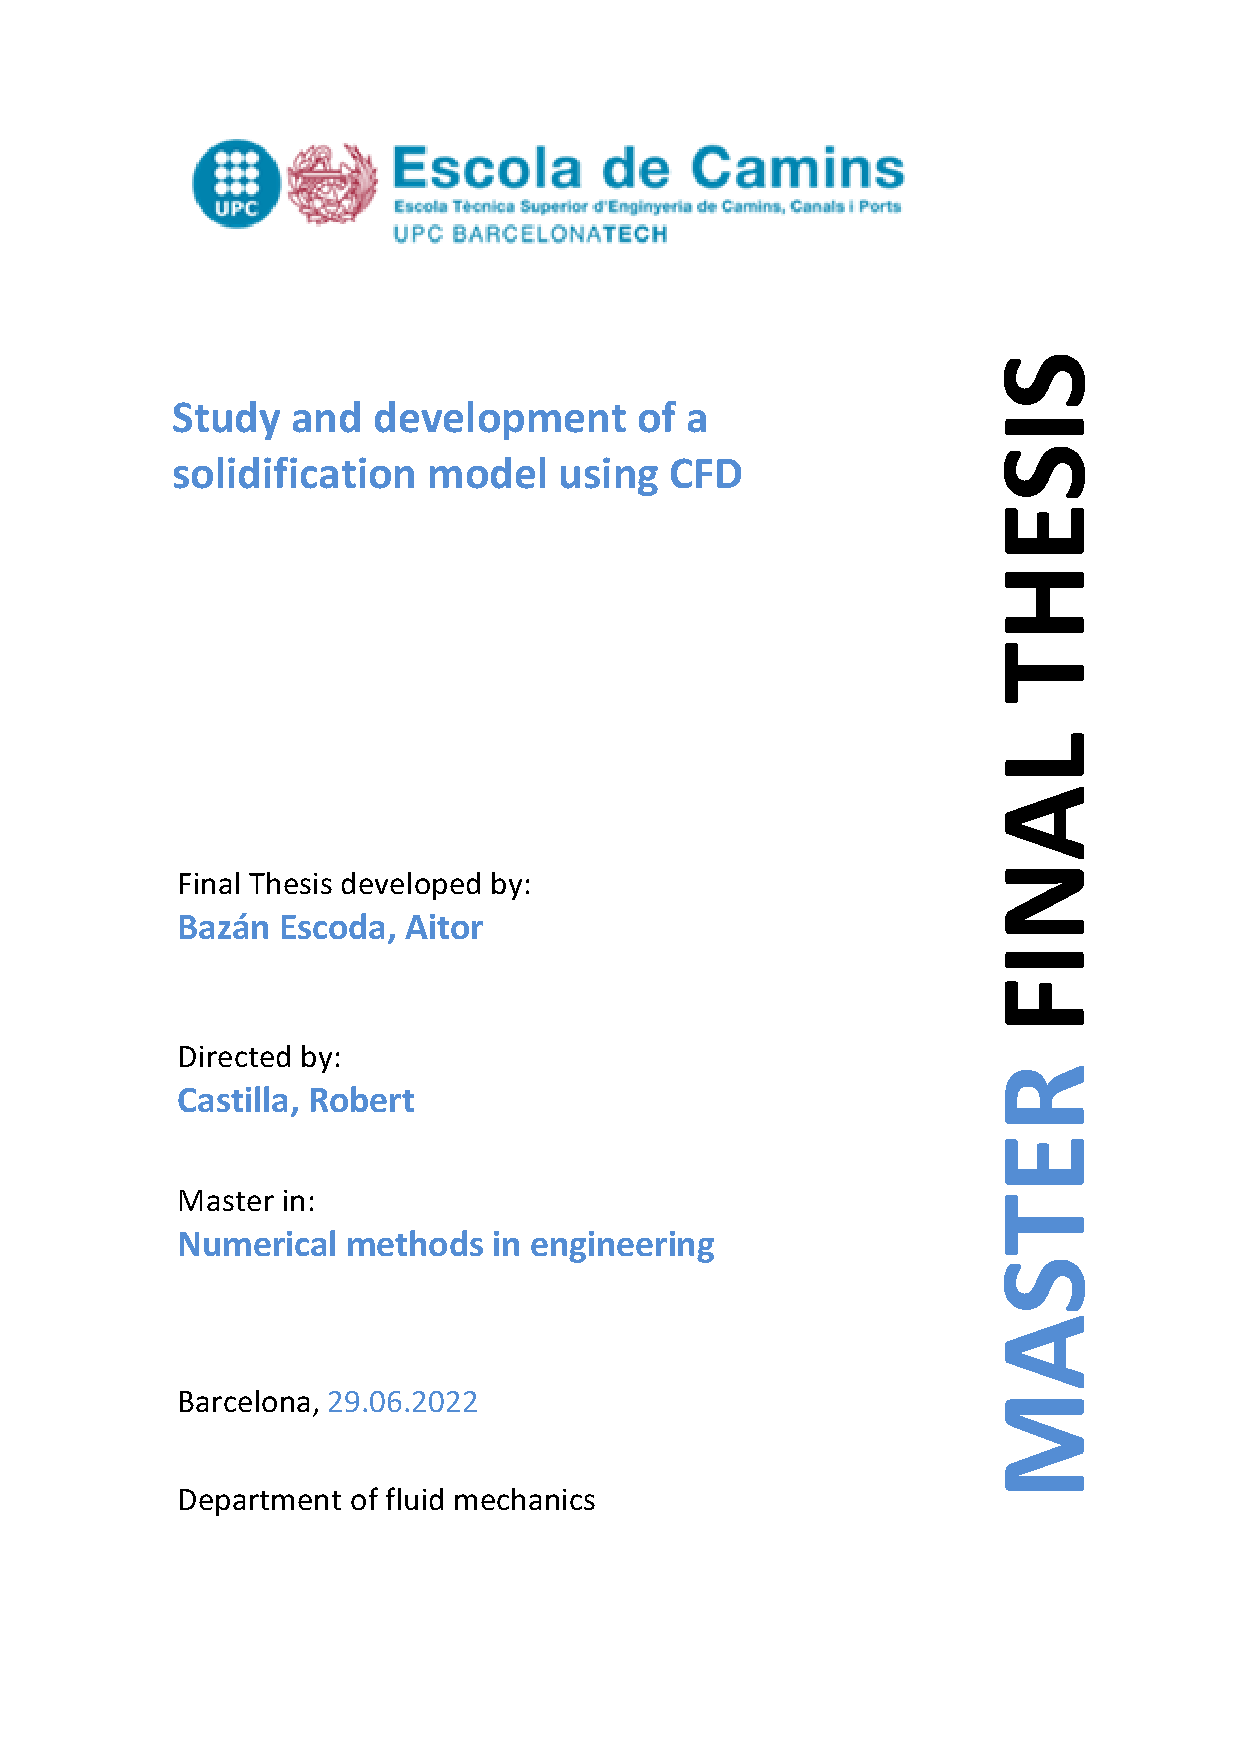
\includepdf[pages=1]{Cover TFM English.pdf}
\frontmatter % Use roman page numbering style (i, ii, iii, iv...) for the pre-content pages

\pagestyle{plain} % Default to the plain heading style until the thesis style is called for the body content

%----------------------------------------------------------------------------------------
%	TITLE PAGE
%----------------------------------------------------------------------------------------

\begin{titlepage}
\begin{center}

\vspace*{.06\textheight}
{\scshape\LARGE \univname\par}\vspace{1.5cm} % University name
\textsc{\Large Master Thesis}\\[0.5cm] % Thesis type

\HRule \\[0.4cm] % Horizontal line
{\huge \bfseries \ttitle\par}\vspace{0.4cm} % Thesis title
\HRule \\[1.5cm] % Horizontal line
 
\begin{minipage}[t]{0.4\textwidth}
\begin{flushleft} \large
\emph{Author:}\\
\href{http://www.johnsmith.com}{\authorname} % Author name - remove the \href bracket to remove the link
\end{flushleft}
\end{minipage}
\begin{minipage}[t]{0.4\textwidth}
\begin{flushright} \large
\emph{Supervisor:} \\
\href{http://www.jamessmith.com}{\supname} % Supervisor name - remove the \href bracket to remove the link  
\end{flushright}
\end{minipage}\\[3cm]
 
\vfill

\large \textit{A thesis submitted in fulfillment of the requirements\\ for the degree of \degreename}\\[0.3cm] % University requirement text
\textit{in the}\\[0.4cm]
\groupname\\\deptname\\[2cm] % Research group name and department name
 
\vfill

{\large \today}\\[4cm] % Date
%\includegraphics{Logo} % University/department logo - uncomment to place it
 
\vfill
\end{center}
\end{titlepage}

%----------------------------------------------------------------------------------------
%	DECLARATION PAGE
%----------------------------------------------------------------------------------------

\begin{declaration}
\addchaptertocentry{\authorshipname} % Add the declaration to the table of contents
\noindent I, \authorname, declare that this thesis titled, \enquote{\ttitle} and the work presented in it are my own. I confirm that:

\begin{itemize} 
\item This work was done wholly or mainly while in candidature for a research degree at this University.
\item Where any part of this thesis has previously been submitted for a degree or any other qualification at this University or any other institution, this has been clearly stated.
\item Where I have consulted the published work of others, this is always clearly attributed.
\item Where I have quoted from the work of others, the source is always given. With the exception of such quotations, this thesis is entirely my own work.
\item I have acknowledged all main sources of help.
\item Where the thesis is based on work done by myself jointly with others, I have made clear exactly what was done by others and what I have contributed myself.\\
\end{itemize}
 
\noindent Signed:\\
\rule[0.5em]{25em}{0.5pt} % This prints a line for the signature
 
\noindent Date:\\
\rule[0.5em]{25em}{0.5pt} % This prints a line to write the date
\end{declaration}

\cleardoublepage

%----------------------------------------------------------------------------------------
%	ABSTRACT PAGE
%----------------------------------------------------------------------------------------

\begin{abstract}
\addchaptertocentry{\abstractname} % Add the abstract to the table of contents
\indent Phase change materials (PCMs) are of great interest within the automotive industry field. Not only when used in thermal management applications but also in different areas where these materials are of vital importance for both a safe and comfortable driving. For such objective, the present project arises from the idea of understanding solidification processes in such areas. In this context, this master's thesis produces a comprehensive state of the art of some of the current numerical methods to effectively represent water solidification. 

\noindent An OpenFOAM 21.12. solver based on a multi-phase solver, multicomponent incompressible solver based on a volume of fluid method is adapted to deal with diffusive-convective phase change. So as to reach this goal, an implementation of the enthalpy-porosity techinque is carried out. The work of Voller is closely followed, and a detailed explanation of the used equations and the assumptions taken is given. Validation of the model is accomplished by comparing the numerical results with the authors in Bourdillon and Kowaleski.

\noindent On a second stage, a 2D semi-empirical model based on the work of Lee is adapted to account for the nucleation characteristics during the process of the water phase change. Validation of the model is done by comparing the obtained results to Neumann solutions for classical Stefan problem. 

\noindent Finally, the current work is extended to couple a fluid region in which the liquid undergoes a phase-change and a solid region. This is done in the context of a conjugate heat transfer scenario. 

\textbf{Keywords:} PCMs, multip-phase, Enthalpy-porosity technique, Voller, Lee model, Stefan problem, conjugate heat transfer, OpenFOAM.
\end{abstract}

%----------------------------------------------------------------------------------------
%	ACKNOWLEDGEMENTS
%----------------------------------------------------------------------------------------

\begin{acknowledgements}
\addchaptertocentry{\acknowledgementname} % Add the acknowledgements to the table of contents
My first and biggest thanks goes to my supervisors, Dr. Robert Castilla and Dr. Gustavo Raush for their invaluable help throughout this work. 
\linebreak
I would like to thank my family and all my workmates in Barcelona Technical Center S.L. for giving me support in the darkest hours.
\end{acknowledgements}

%----------------------------------------------------------------------------------------
%	LIST OF CONTENTS/FIGURES/TABLES PAGES
%----------------------------------------------------------------------------------------

\tableofcontents  % Prints the main table of contents

\listoffigures % Prints the list of figures

\listoftables % Prints the list of tables



%-------------------------------------------------------------------
%----------------------------------------------------------------------------------------
%	THESIS CONTENT - CHAPTERS
%----------------------------------------------------------------------------------------

\mainmatter % Begin numeric (1,2,3...) page numbering

\pagestyle{thesis} % Return the page headers back to the "thesis" style

% Include the chapters of the thesis as separate files from the Chapters folder
% Uncomment the lines as you write the chapters

% Chapter 1

\chapter{Introduction} % Main chapter title

\label{Chapter1} % For referencing the chapter elsewhere, use \ref{Chapter1} 

%----------------------------------------------------------------------------------------

% Define some commands to keep the formatting separated from the content 
\newcommand{\keyword}[1]{\textbf{#1}}
\newcommand{\tabhead}[1]{\textbf{#1}}
\newcommand{\code}[1]{\texttt{#1}}
\newcommand{\file}[1]{\texttt{\bfseries#1}}
\newcommand{\option}[1]{\texttt{\itshape#1}}
\setcounter{secnumdepth}{4}
%----------------------------------------------------------------------------------------

\section{Thesis Statement. Background and motivation}

During the last decade, the use of phase change materials has been growing in the automotive industry. \newline
These substances release or absorb large amounts of latent heat when they go through a change in their physical state, as the material reaches its specific phase change temperature. Thus, in the process of latent heat release or absorption, the temperature of the PCM remains constant. Therefore, PCMs are considered to be efficient in terms of thermal storage. \newline
\indent On the other hand, the use of these materials is not exclusive for thermal management. It is of relevant importance when used in conjunction with soap in the windshield wiper system of the car. In such zone, problems involving solidification are of considerable relevance. And this is mainly due to a volumetric expansion originated by the thermal effects within the PCM which at its turn, generates stresses in the polymeric tank in which is bottled up.
\newline
\indent Therefore, this master's thesis main objective aims to study different numerical techniques to represent solidification process and, specially, pure water phase change. This is accomplished by first imlementing an enthalpy-porosity technique within the frame of a multi-phase incompressible solver based on volume-of-fluid (VOF) method for interface tracking. The objective of this first stage is to apply sensible and latent heat as source terms in the energy equation. On a second term, a 2D semi-empirical model based on the work of Lee is adapted to account for the nucleation characteristics occured during the water phase transition. 
\indent The final stage of this thesis is devoted to an implementation of a multiregion solver to calculate conjugate heat transfer problems between solid and fluid zones with the singularity of being, the fluid zone, capable of handling phase change materials. 



%----------------------------------------------------------------------------------------

\section{Phase-Change Process}
A complex interaction of the molecular forces generate water to behave in a curious way when it gets frozen into ice. The vast majority of substances, when they are cooled, become more dense in the frozen state than when liquid. However, when cooled under a specific temperature, water begins to expand and, once it starts freezing, it becomes less dense than water. 
\newline
\subsection{Phase diagram of ice}
Ice crystals undergo different kinds of structures. Called ice Ih, in the form of hexagonal ice and, manifested in six cornered snow flakes, is the natural ice found in earth. However, at lower pressures below 2 kbar, many other ice structures may exist.
\newline
The ice phase diagram shown below, points out the conditions of stability for all ice phases. As it is cleared out, the line between the water and ice Ih is an equilibrium line with a negative slope, consequence of having, the solid, lower density than the liquid. These equilibrium lines extend in the form of metastable phase boundaries into the area of stability of other ice phases.
Although there are at least 11 crystalline ice shapes, the only which is found in naturally on earth is the hexagonal form. 
\newline
As a remark, the implication that there is a rise on the pressure would not propitiate ice formation at 0ºC, instead water would need to be cooled down.
\subsection{Properties of ice}
Ice, when subjected to visible light conditions, is transparent and has the lowest index of refraction for the sodium spectrum of any known crystalline material[].
\newline
Mechanically, ice behaves like a viscoelastic material with a non linear law. Pollycrystalline ice subjected to stress, deforms elastically, followed by a transient creep and finally, a secondary creep in the form of steady viscous flow is obtained.
\newline
As pointed out in [], the surface of ice Ih near the melting point has many dangling broken bounds that boost the presence of a liquid-like layer and as a consequence, low friction on such surface. Variation of density of ice with phase at 110 K and some physical properties of ice Ih at 0ºC are described in the tables below.
\newline

\subsection{Freezing phenomena}
Time-temperature diagram for freezing of pure water (ABCDE) and aqueous solutions (AB'C'D'E') show the physical process that occurs during the solidification. The first stage, from A to B, belongs to undercooling, also called supercooling, and it is arisen below the freezing point $T_f$, which is equal to the melting point, $T_m$. This point is referred to a non equilibrium point and it is analogous to an activation energy necessary for the nucleation process. Before nucleation process, pure water may need to be cooled down several degrees. At point B, the system nucleates and releases its latent heat faster than the heat which is being removed from itself.
\newline
From C to D, the horizontal axis shows the evolution of the crystal growth in time. At C, there exists the nucleation point and, from there through D, latent heat gets removed out of the system at constant temperature. In this way, the mixture, which is in a partially frozen state, does not cool until all the potentially freezable water has crystallized.


\begin{figure}[h]
	\label{fig:boat1}
	\centering	
	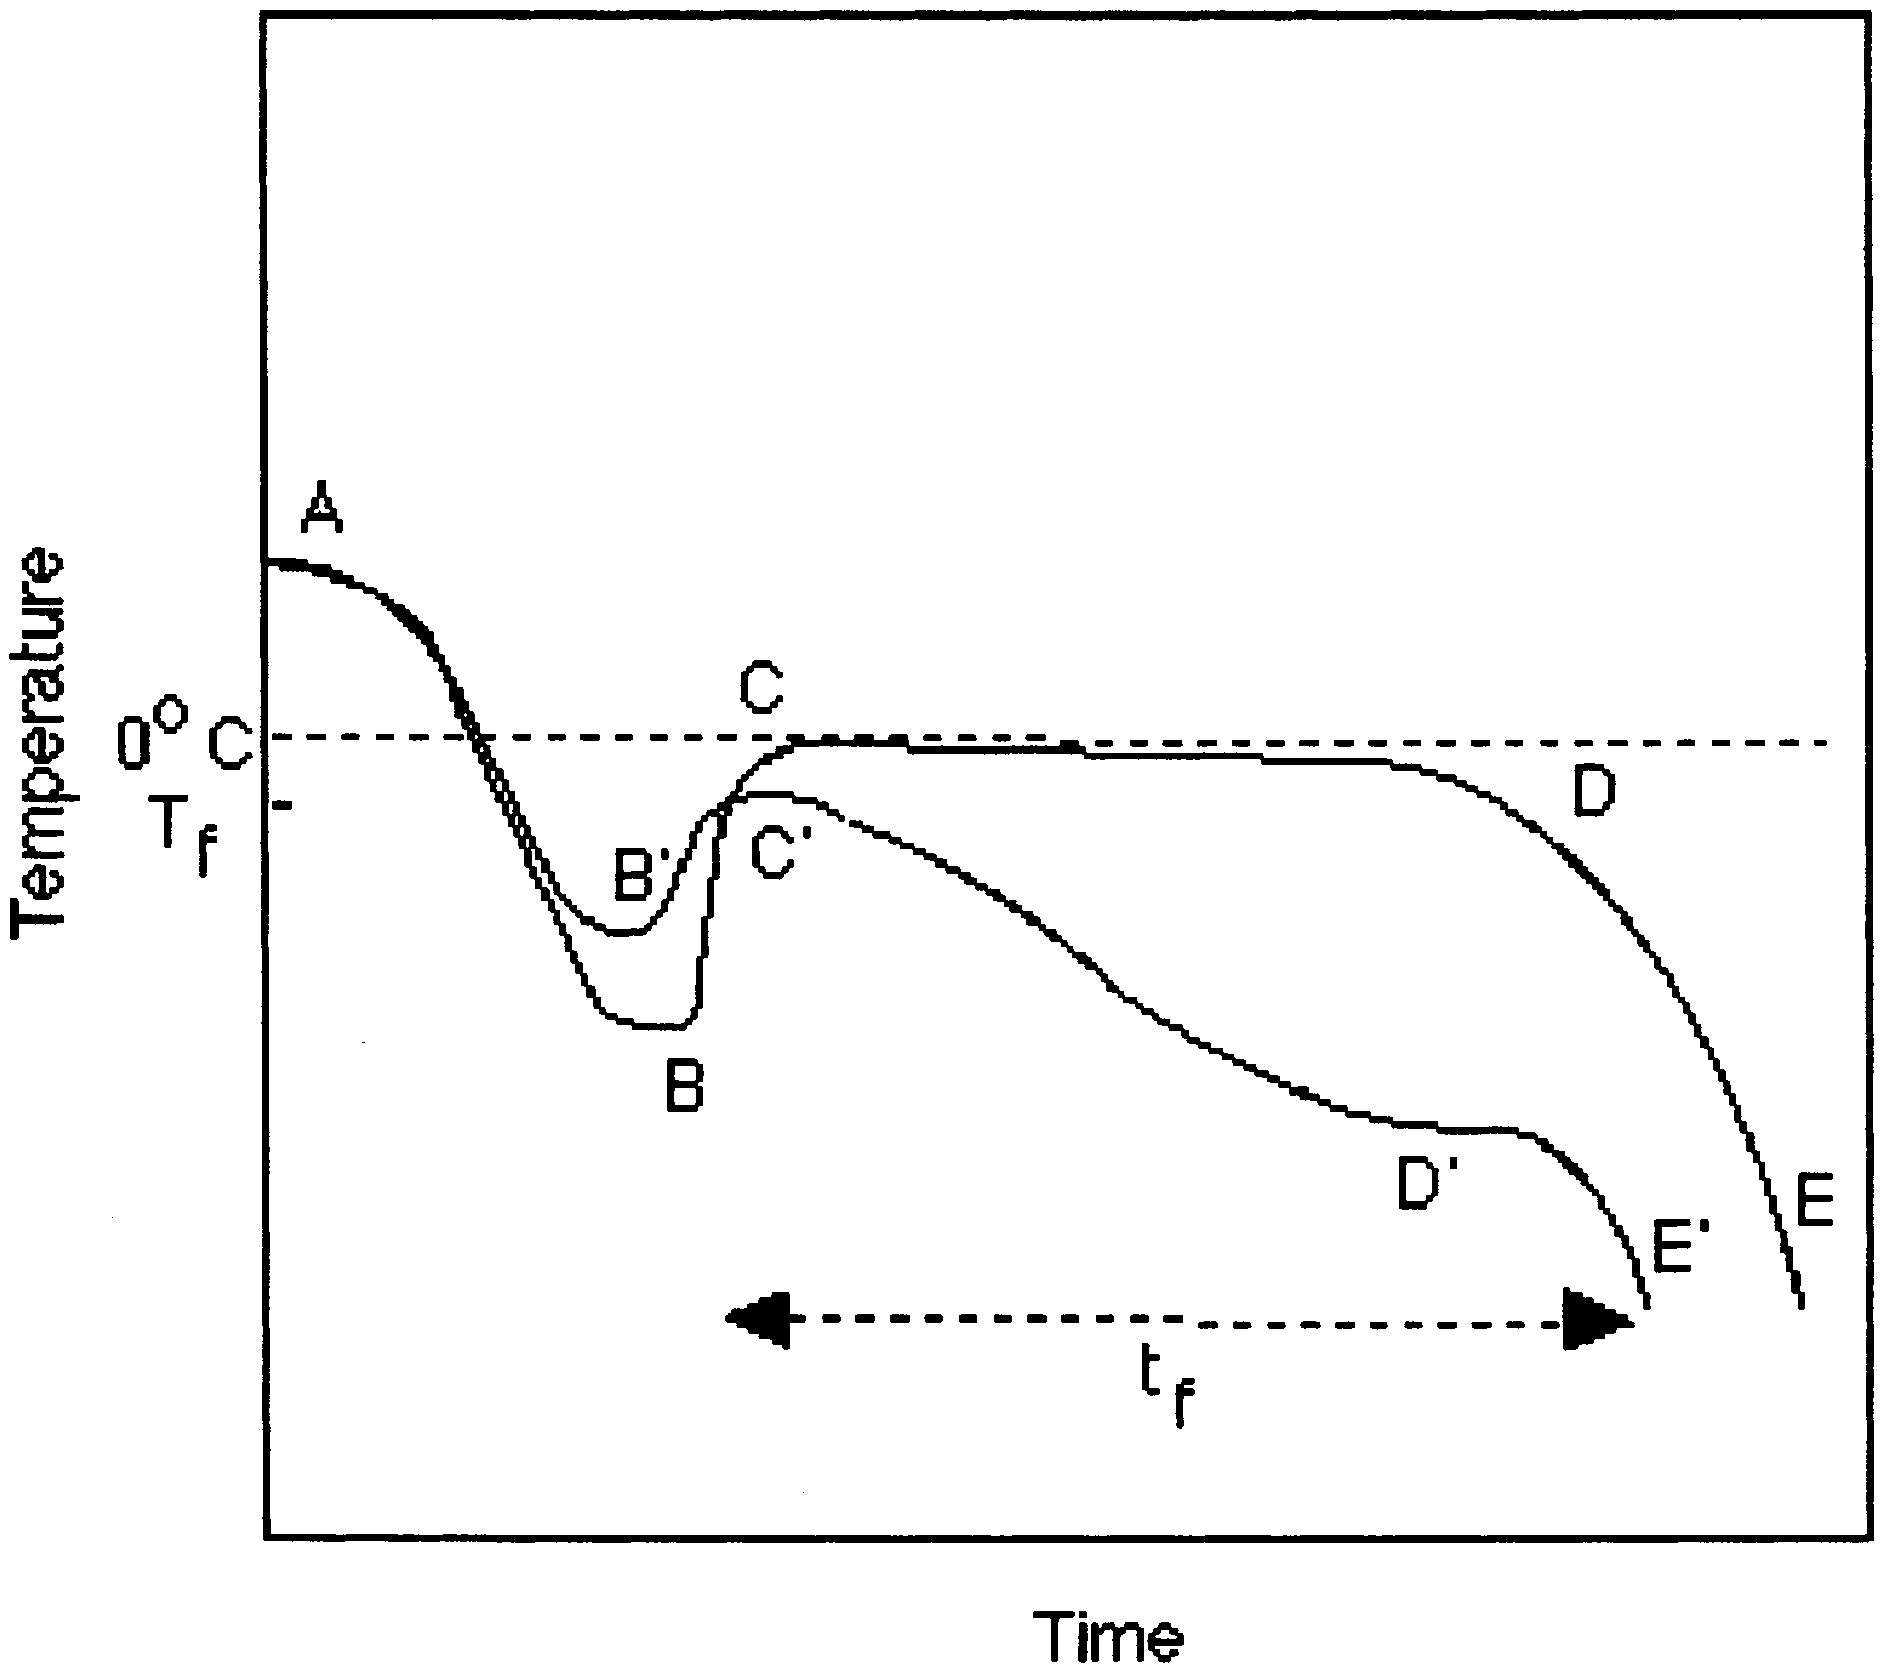
\includegraphics[width=0.6\textwidth]{crystallization_of_water.png}
	\caption{Process of crystallization of water.}
\end{figure} 

\section{Mechanisms of Heat Transfer. Heat convection}
The process of water freezing in enclosures is common in engineering. When there exist temperature gradients within the liquid phase in the process of solidification, a natural buoyancy driven flow is initiated and such behavior is determined to affect the shape of the liquid/solid interface as well as the progress of solidification.
\newline
Indeed, these temperature differences in the liquid cause density variations so that the natural motion occurs. Boussinesq approximation can be validly used for fluids whose density varies linearly with temperature. However, pure water exhibits a maximum in its density when it ranges between 0ºC and 4ºC. Beyond this last temperature, and known as density inversion point, density decreases in a nonlinear manner as the temperature passes through the freezing point. In convective heat transfer, surroundings of the temperature where the aforementioned maximum happens to be, behave in a complex manner leading to fully control the process of growth of the solid phase.
\newline

\subsection{Stefan Problem}

%%TO BE IMPLEMENTED AT THE END
\section{Conjugate Heat Transfer. Heat conduction}

\subsection{Governing Equations}
\subsubsection{Governing Equations for the Fluid}

\subsubsection{Governing Equations for the Solid}

\begin{equation}
	\frac{\partial}{\partial x_{i}}\left(\rho u_{i} T\right)=\frac{\partial}{\partial x_{i}}\left(\frac{k}{C_{p}} \frac{\partial u_{j}}{\partial x_{j}}\right)
\end{equation}
%----------------------------------------------------------------------------------------
%
%\section{Getting Started with this Template}
%
%If you are familiar with \LaTeX{}, then you should explore the directory structure of the template and then proceed to place your own information into the \emph{THESIS INFORMATION} block of the \file{main.tex} file. You can then modify the rest of this file to your unique specifications based on your degree/university. Section \ref{FillingFile} on page \pageref{FillingFile} will help you do this. Make sure you also read section \ref{ThesisConventions} about thesis conventions to get the most out of this template.

%If you are new to \LaTeX{} it is recommended that you carry on reading through the rest of the information in this document.
%
%Before you begin using this template you should ensure that its style complies with the thesis style guidelines imposed by your institution. In most cases this template style and layout will be suitable. If it is not, it may only require a small change to bring the template in line with your institution's recommendations. These modifications will need to be done on the \file{MastersDoctoralThesis.cls} file.
%
%\subsection{About this Template}
%
%This \LaTeX{} Thesis Template is originally based and created around a \LaTeX{} style file created by Steve R.\ Gunn from the University of Southampton (UK), department of Electronics and Computer Science. You can find his original thesis style file at his site, here:
%\url{http://www.ecs.soton.ac.uk/~srg/softwaretools/document/templates/}
%
%Steve's \file{ecsthesis.cls} was then taken by Sunil Patel who modified it by creating a skeleton framework and folder structure to place the thesis files in. The resulting template can be found on Sunil's site here:
%\url{http://www.sunilpatel.co.uk/thesis-template}
%
%Sunil's template was made available through \url{http://www.LaTeXTemplates.com} where it was modified many times based on user requests and questions. Version 2.0 and onwards of this template represents a major modification to Sunil's template and is, in fact, hardly recognisable. The work to make version 2.0 possible was carried out by \href{mailto:vel@latextemplates.com}{Vel} and Johannes Böttcher.
%
%%----------------------------------------------------------------------------------------
%
%\section{What this Template Includes}
%
%\subsection{Folders}
%
%This template comes as a single zip file that expands out to several files and folders. The folder names are mostly self-explanatory:
%
%\keyword{Appendices} -- this is the folder where you put the appendices. Each appendix should go into its own separate \file{.tex} file. An example and template are included in the directory.
%
%\keyword{Chapters} -- this is the folder where you put the thesis chapters. A thesis usually has about six chapters, though there is no hard rule on this. Each chapter should go in its own separate \file{.tex} file and they can be split as:
%\begin{itemize}
%\item Chapter 1: Introduction to the thesis topic
%\item Chapter 2: Background information and theory
%\item Chapter 3: (Laboratory) experimental setup
%\item Chapter 4: Details of experiment 1
%\item Chapter 5: Details of experiment 2
%\item Chapter 6: Discussion of the experimental results
%\item Chapter 7: Conclusion and future directions
%\end{itemize}
%This chapter layout is specialised for the experimental sciences, your discipline may be different.
%
%\keyword{Figures} -- this folder contains all figures for the thesis. These are the final images that will go into the thesis document.
%
%\subsection{Files}
%
%Included are also several files, most of them are plain text and you can see their contents in a text editor. After initial compilation, you will see that more auxiliary files are created by \LaTeX{} or BibTeX and which you don't need to delete or worry about:
%
%\keyword{example.bib} -- this is an important file that contains all the bibliographic information and references that you will be citing in the thesis for use with BibTeX. You can write it manually, but there are reference manager programs available that will create and manage it for you. Bibliographies in \LaTeX{} are a large subject and you may need to read about BibTeX before starting with this. Many modern reference managers will allow you to export your references in BibTeX format which greatly eases the amount of work you have to do.
%
%\keyword{MastersDoctoralThesis.cls} -- this is an important file. It is the class file that tells \LaTeX{} how to format the thesis. 
%
%\keyword{main.pdf} -- this is your beautifully typeset thesis (in the PDF file format) created by \LaTeX{}. It is supplied in the PDF with the template and after you compile the template you should get an identical version.
%
%\keyword{main.tex} -- this is an important file. This is the file that you tell \LaTeX{} to compile to produce your thesis as a PDF file. It contains the framework and constructs that tell \LaTeX{} how to layout the thesis. It is heavily commented so you can read exactly what each line of code does and why it is there. After you put your own information into the \emph{THESIS INFORMATION} block -- you have now started your thesis!
%
%Files that are \emph{not} included, but are created by \LaTeX{} as auxiliary files include:
%
%\keyword{main.aux} -- this is an auxiliary file generated by \LaTeX{}, if it is deleted \LaTeX{} simply regenerates it when you run the main \file{.tex} file.
%
%\keyword{main.bbl} -- this is an auxiliary file generated by BibTeX, if it is deleted, BibTeX simply regenerates it when you run the \file{main.aux} file. Whereas the \file{.bib} file contains all the references you have, this \file{.bbl} file contains the references you have actually cited in the thesis and is used to build the bibliography section of the thesis.
%
%\keyword{main.blg} -- this is an auxiliary file generated by BibTeX, if it is deleted BibTeX simply regenerates it when you run the main \file{.aux} file.
%
%\keyword{main.lof} -- this is an auxiliary file generated by \LaTeX{}, if it is deleted \LaTeX{} simply regenerates it when you run the main \file{.tex} file. It tells \LaTeX{} how to build the \emph{List of Figures} section.
%
%\keyword{main.log} -- this is an auxiliary file generated by \LaTeX{}, if it is deleted \LaTeX{} simply regenerates it when you run the main \file{.tex} file. It contains messages from \LaTeX{}, if you receive errors and warnings from \LaTeX{}, they will be in this \file{.log} file.
%
%\keyword{main.lot} -- this is an auxiliary file generated by \LaTeX{}, if it is deleted \LaTeX{} simply regenerates it when you run the main \file{.tex} file. It tells \LaTeX{} how to build the \emph{List of Tables} section.
%
%\keyword{main.out} -- this is an auxiliary file generated by \LaTeX{}, if it is deleted \LaTeX{} simply regenerates it when you run the main \file{.tex} file.
%
%So from this long list, only the files with the \file{.bib}, \file{.cls} and \file{.tex} extensions are the most important ones. The other auxiliary files can be ignored or deleted as \LaTeX{} and BibTeX will regenerate them.
%
%%----------------------------------------------------------------------------------------
%
%\section{Filling in Your Information in the \file{main.tex} File}\label{FillingFile}
%
%You will need to personalise the thesis template and make it your own by filling in your own information. This is done by editing the \file{main.tex} file in a text editor or your favourite LaTeX environment.
%
%Open the file and scroll down to the third large block titled \emph{THESIS INFORMATION} where you can see the entries for \emph{University Name}, \emph{Department Name}, etc \ldots
%
%Fill out the information about yourself, your group and institution. You can also insert web links, if you do, make sure you use the full URL, including the \code{http://} for this. If you don't want these to be linked, simply remove the \verb|\href{url}{name}| and only leave the name.
%
%When you have done this, save the file and recompile \code{main.tex}. All the information you filled in should now be in the PDF, complete with web links. You can now begin your thesis proper!
%
%%----------------------------------------------------------------------------------------
%
%\section{The \code{main.tex} File Explained}
%
%The \file{main.tex} file contains the structure of the thesis. There are plenty of written comments that explain what pages, sections and formatting the \LaTeX{} code is creating. Each major document element is divided into commented blocks with titles in all capitals to make it obvious what the following bit of code is doing. Initially there seems to be a lot of \LaTeX{} code, but this is all formatting, and it has all been taken care of so you don't have to do it.
%
%Begin by checking that your information on the title page is correct. For the thesis declaration, your institution may insist on something different than the text given. If this is the case, just replace what you see with what is required in the \emph{DECLARATION PAGE} block.
%
%Then comes a page which contains a funny quote. You can put your own, or quote your favourite scientist, author, person, and so on. Make sure to put the name of the person who you took the quote from.
%
%Following this is the abstract page which summarises your work in a condensed way and can almost be used as a standalone document to describe what you have done. The text you write will cause the heading to move up so don't worry about running out of space.
%
%Next come the acknowledgements. On this page, write about all the people who you wish to thank (not forgetting parents, partners and your advisor/supervisor).
%
%The contents pages, list of figures and tables are all taken care of for you and do not need to be manually created or edited. The next set of pages are more likely to be optional and can be deleted since they are for a more technical thesis: insert a list of abbreviations you have used in the thesis, then a list of the physical constants and numbers you refer to and finally, a list of mathematical symbols used in any formulae. Making the effort to fill these tables means the reader has a one-stop place to refer to instead of searching the internet and references to try and find out what you meant by certain abbreviations or symbols.
%
%The list of symbols is split into the Roman and Greek alphabets. Whereas the abbreviations and symbols ought to be listed in alphabetical order (and this is \emph{not} done automatically for you) the list of physical constants should be grouped into similar themes.
%
%The next page contains a one line dedication. Who will you dedicate your thesis to?
%
%Finally, there is the block where the chapters are included. Uncomment the lines (delete the \code{\%} character) as you write the chapters. Each chapter should be written in its own file and put into the \emph{Chapters} folder and named \file{Chapter1}, \file{Chapter2}, etc\ldots Similarly for the appendices, uncomment the lines as you need them. Each appendix should go into its own file and placed in the \emph{Appendices} folder.
%
%After the preamble, chapters and appendices finally comes the bibliography. The bibliography style (called \option{authoryear}) is used for the bibliography and is a fully featured style that will even include links to where the referenced paper can be found online. Do not underestimate how grateful your reader will be to find that a reference to a paper is just a click away. Of course, this relies on you putting the URL information into the BibTeX file in the first place.
%
%%----------------------------------------------------------------------------------------
%
%\section{Thesis Features and Conventions}\label{ThesisConventions}
%
%To get the best out of this template, there are a few conventions that you may want to follow.
%
%One of the most important (and most difficult) things to keep track of in such a long document as a thesis is consistency. Using certain conventions and ways of doing things (such as using a Todo list) makes the job easier. Of course, all of these are optional and you can adopt your own method.
%
%\subsection{Printing Format}
%
%This thesis template is designed for double sided printing (i.e. content on the front and back of pages) as most theses are printed and bound this way. Switching to one sided printing is as simple as uncommenting the \option{oneside} option of the \code{documentclass} command at the top of the \file{main.tex} file. You may then wish to adjust the margins to suit specifications from your institution.
%
%The headers for the pages contain the page number on the outer side (so it is easy to flick through to the page you want) and the chapter name on the inner side.
%
%The text is set to 11 point by default with single line spacing, again, you can tune the text size and spacing should you want or need to using the options at the very start of \file{main.tex}. The spacing can be changed similarly by replacing the \option{singlespacing} with \option{onehalfspacing} or \option{doublespacing}.
%
%\subsection{Using US Letter Paper}
%
%The paper size used in the template is A4, which is the standard size in Europe. If you are using this thesis template elsewhere and particularly in the United States, then you may have to change the A4 paper size to the US Letter size. This can be done in the margins settings section in \file{main.tex}.
%
%Due to the differences in the paper size, the resulting margins may be different to what you like or require (as it is common for institutions to dictate certain margin sizes). If this is the case, then the margin sizes can be tweaked by modifying the values in the same block as where you set the paper size. Now your document should be set up for US Letter paper size with suitable margins.
%
%\subsection{References}
%
%The \code{biblatex} package is used to format the bibliography and inserts references such as this one \parencite{Reference1}. The options used in the \file{main.tex} file mean that the in-text citations of references are formatted with the author(s) listed with the date of the publication. Multiple references are separated by semicolons (e.g. \parencite{Reference2, Reference1}) and references with more than three authors only show the first author with \emph{et al.} indicating there are more authors (e.g. \parencite{Reference3}). This is done automatically for you. To see how you use references, have a look at the \file{Chapter1.tex} source file. Many reference managers allow you to simply drag the reference into the document as you type.
%
%Scientific references should come \emph{before} the punctuation mark if there is one (such as a comma or period). The same goes for footnotes\footnote{Such as this footnote, here down at the bottom of the page.}. You can change this but the most important thing is to keep the convention consistent throughout the thesis. Footnotes themselves should be full, descriptive sentences (beginning with a capital letter and ending with a full stop). The APA6 states: \enquote{Footnote numbers should be superscripted, [...], following any punctuation mark except a dash.} The Chicago manual of style states: \enquote{A note number should be placed at the end of a sentence or clause. The number follows any punctuation mark except the dash, which it precedes. It follows a closing parenthesis.}
%
%The bibliography is typeset with references listed in alphabetical order by the first author's last name. This is similar to the APA referencing style. To see how \LaTeX{} typesets the bibliography, have a look at the very end of this document (or just click on the reference number links in in-text citations).
%
%\subsubsection{A Note on bibtex}
%
%The bibtex backend used in the template by default does not correctly handle unicode character encoding (i.e. "international" characters). You may see a warning about this in the compilation log and, if your references contain unicode characters, they may not show up correctly or at all. The solution to this is to use the biber backend instead of the outdated bibtex backend. This is done by finding this in \file{main.tex}: \option{backend=bibtex} and changing it to \option{backend=biber}. You will then need to delete all auxiliary BibTeX files and navigate to the template directory in your terminal (command prompt). Once there, simply type \code{biber main} and biber will compile your bibliography. You can then compile \file{main.tex} as normal and your bibliography will be updated. An alternative is to set up your LaTeX editor to compile with biber instead of bibtex, see \href{http://tex.stackexchange.com/questions/154751/biblatex-with-biber-configuring-my-editor-to-avoid-undefined-citations/}{here} for how to do this for various editors.
%
%\subsection{Tables}
%
%Tables are an important way of displaying your results, below is an example table which was generated with this code:
%
%{\small
%\begin{verbatim}
%\begin{table}
%\caption{The effects of treatments X and Y on the four groups studied.}
%\label{tab:treatments}
%\centering
%\begin{tabular}{l l l}
%\toprule
%\tabhead{Groups} & \tabhead{Treatment X} & \tabhead{Treatment Y} \\
%\midrule
%1 & 0.2 & 0.8\\
%2 & 0.17 & 0.7\\
%3 & 0.24 & 0.75\\
%4 & 0.68 & 0.3\\
%\bottomrule\\
%\end{tabular}
%\end{table}
%\end{verbatim}
%}
%
%\begin{table}
%\caption{The effects of treatments X and Y on the four groups studied.}
%\label{tab:treatments}
%\centering
%\begin{tabular}{l l l}
%\toprule
%\tabhead{Groups} & \tabhead{Treatment X} & \tabhead{Treatment Y} \\
%\midrule
%1 & 0.2 & 0.8\\
%2 & 0.17 & 0.7\\
%3 & 0.24 & 0.75\\
%4 & 0.68 & 0.3\\
%\bottomrule\\
%\end{tabular}
%\end{table}
%
%You can reference tables with \verb|\ref{<label>}| where the label is defined within the table environment. See \file{Chapter1.tex} for an example of the label and citation (e.g. Table~\ref{tab:treatments}).
%
%\subsection{Figures}
%
%There will hopefully be many figures in your thesis (that should be placed in the \emph{Figures} folder). The way to insert figures into your thesis is to use a code template like this:
%\begin{verbatim}
%\begin{figure}
%\centering
%
\includegraphics{Figures/Electron}
%\decoRule
%\caption[An Electron]{An electron (artist's impression).}
%\label{fig:Electron}
%\end{figure}
%\end{verbatim}
%Also look in the source file. Putting this code into the source file produces the picture of the electron that you can see in the figure below.
%
%\begin{figure}[th]
%\centering
%
\includegraphics{Figures/Electron}
%\decoRule
%\caption[An Electron]{An electron (artist's impression).}
%\label{fig:Electron}
%\end{figure}
%
%Sometimes figures don't always appear where you write them in the source. The placement depends on how much space there is on the page for the figure. Sometimes there is not enough room to fit a figure directly where it should go (in relation to the text) and so \LaTeX{} puts it at the top of the next page. Positioning figures is the job of \LaTeX{} and so you should only worry about making them look good!
%
%Figures usually should have captions just in case you need to refer to them (such as in Figure~\ref{fig:Electron}). The \verb|\caption| command contains two parts, the first part, inside the square brackets is the title that will appear in the \emph{List of Figures}, and so should be short. The second part in the curly brackets should contain the longer and more descriptive caption text.
%
%The \verb|\decoRule| command is optional and simply puts an aesthetic horizontal line below the image. If you do this for one image, do it for all of them.
%
%\LaTeX{} is capable of using images in pdf, jpg and png format.
%
%\subsection{Typesetting mathematics}
%
%If your thesis is going to contain heavy mathematical content, be sure that \LaTeX{} will make it look beautiful, even though it won't be able to solve the equations for you.
%
%The \enquote{Not So Short Introduction to \LaTeX} (available on \href{http://www.ctan.org/tex-archive/info/lshort/english/lshort.pdf}{CTAN}) should tell you everything you need to know for most cases of typesetting mathematics. If you need more information, a much more thorough mathematical guide is available from the AMS called, \enquote{A Short Math Guide to \LaTeX} and can be downloaded from:
%\url{ftp://ftp.ams.org/pub/tex/doc/amsmath/short-math-guide.pdf}
%
%There are many different \LaTeX{} symbols to remember, luckily you can find the most common symbols in \href{http://ctan.org/pkg/comprehensive}{The Comprehensive \LaTeX~Symbol List}.
%
%You can write an equation, which is automatically given an equation number by \LaTeX{} like this:
%\begin{verbatim}
%\begin{equation}
%E = mc^{2}
%\label{eqn:Einstein}
%\end{equation}
%\end{verbatim}
%
%This will produce Einstein's famous energy-matter equivalence equation:
%\begin{equation}
%E = mc^{2}
%\label{eqn:Einstein}
%\end{equation}
%
%All equations you write (which are not in the middle of paragraph text) are automatically given equation numbers by \LaTeX{}. If you don't want a particular equation numbered, use the unnumbered form:
%\begin{verbatim}
%\[ a^{2}=4 \]
%\end{verbatim}
%
%%----------------------------------------------------------------------------------------
%
%\section{Sectioning and Subsectioning}
%
%You should break your thesis up into nice, bite-sized sections and subsections. \LaTeX{} automatically builds a table of Contents by looking at all the \verb|\chapter{}|, \verb|\section{}|  and \verb|\subsection{}| commands you write in the source.
%
%The Table of Contents should only list the sections to three (3) levels. A \verb|chapter{}| is level zero (0). A \verb|\section{}| is level one (1) and so a \verb|\subsection{}| is level two (2). In your thesis it is likely that you will even use a \verb|subsubsection{}|, which is level three (3). The depth to which the Table of Contents is formatted is set within \file{MastersDoctoralThesis.cls}. If you need this changed, you can do it in \file{main.tex}.
%
%%----------------------------------------------------------------------------------------
%
%\section{In Closing}
%
%You have reached the end of this mini-guide. You can now rename or overwrite this pdf file and begin writing your own \file{Chapter1.tex} and the rest of your thesis. The easy work of setting up the structure and framework has been taken care of for you. It's now your job to fill it out!
%
%Good luck and have lots of fun!
%
%\begin{flushright}
%Guide written by ---\\
%Sunil Patel: \href{http://www.sunilpatel.co.uk}{www.sunilpatel.co.uk}\\
%Vel: \href{http://www.LaTeXTemplates.com}{LaTeXTemplates.com}
%\end{flushright}

% Chapter 1

\chapter{Numerical Methods for Phase-Change Phenomena} % Main chapter title

\label{Chapter2} % For referencing the chapter elsewhere, use \ref{Chapter1} 

%----------------------------------------------------------------------------------------

% Define some commands to keep the formatting separated from the content 
\section{State of Art. Numerical Methods} %Description of general numerical methods for phase change 
Considering the PCM density as constant in the model might be thought as a reasonable assumption in some cases, in others where thermo-mechanical coupling between the fluid and its container is intended, it makes impossible to account for some physical behaviors which may result from expansion or contraction during the phase change of the material. However, the main goal of this thesis is not to present a method that represents thermo-mechanical coupling but a technique that ensures volume expansion due to density changes through the fluid domain.
To reach this point, it is important to point some of the numerous researches that have been conducted in order to investigate the problem of solidification and melting. 
\newline

At the present, the main numerical methods representing the treatment of liquid-solid phase change are divided into these categories:
\begin{itemize}
	\item Surface tracking methods,
	\item Volume tracking methods,
	\item Moving mesh methods,
\end{itemize}
\subsection*{Surface tracking methods}

\subsection*{Volume tracking methods}

\subsection*{Moving mesh methods}

\section{Solidification methods}
The challenge of a numerical investigation of a solidification process is to capture the free surface for the flow of the phase change material and, at the same time, account for the moving boundary induced by the phase change within the PCM. The free surface may be handled by the volume-of-fluid (VOF), originally introduced by [ref Hirt]. VOF relies on the definition of a transport indicator function within the finite volume method's framework.
Simultaneously, and in order to account for the phase changes, some of the used models are based on meso-scale. This is the phenomena occurring between microscopic and continuum length scales and, in the current context, the complex micro structure generated during the solidification is approximated as liquid, mushy (intermediate state), and solid regions. Mushy region is thereby described as an averaged value of the liquid and solid properties.
\newline
\indent One of the most used methods is the enthalpy-porosity technique, originally developed by Voller and Prakash [ref. Voller], which uses the typical conservation equations on a fixed Eulerian grid. The main concepts underlaying such method are: on the one side, an additional source term to the energy conservation equation is applied to describe the release of latent heat. On the other side, the solidification effects on the mass transport are modelled as a porosity variable and this is introduced as a Darcy-type source term to the momentum equation.
\newline
\indent Some of the studies found on this topic, the coupling of both VOF and enthalpy-porosity methods are mainly related to casting processes. Rösler and Brüggermann [ref] introduced a numerical model for a solid-liquid phase change inside a latent heat thermal energy storage. Richter et al. [ref] worked out a method for the simultaneous moult filling and solidification process which settles the developing of free surface flow and the liquid-solid phase transition under the volume-of-fluid and enthalpy-porosity methods.
However, no adaptation of these methods to purely solidification processes has been found. Therefore, and, the objectives of this research are:
\begin{itemize}
	\item To introduce a new solver based on the coupling of VOF and enthalpy-porosity techniques which covers the relevant physical effects during the process of solidification.
	\item	To validate simulation results by using benchmark cases found in the literature.
\end{itemize}
Numerical methods commented are briefly described next.

%% Present Lee model
On the other hand, semi-empirical methods ...
\subsection{Volume-of-Fluid Method: General Aspects}
The volume of fluid method takes relevance when fluids coexist with other phases. An example could be the ice (solid phase) advancing front within the liquid phase. The surface in between both phases needs to be solved by means of the volume of fluid technique.
\newline
This is sometimes seen as the conservation of the mixture components along the path of a fluid region. The equation which allows that is described as:
\begin{equation}
	\frac{\partial \gamma_{\text {phase }}}{\partial t}+\frac{\partial\left(\gamma_{\text {phase }} u_{j}\right)}{\partial x_{j}}=0
	\label{2.1}
\end{equation}
In which $\alpha_{phase}$ corresponds to the phase fraction and it applies
\begin{equation}
	\gamma_{phase}= \begin{cases}
		0 & =\text { solid PCM } \\ 0<\gamma_{phase}<1 & =\text { cell contains the interface } \\ 1 & =\text { liquid } \mathrm{PCM}
	\end{cases}
	\label{2.2}
\end{equation}

\subsection{Enthalpy-Porosity Model. Governing Equations}
The energy equation based on the enthalpy formulation for convective-diffusive heat transfer states that,
\begin{equation}
	\frac{\partial \rho h}{\partial t}+\frac{\partial}{\partial x_{j}}\left(\rho u_{j} h\right)=\frac{\partial}{\partial x_{j}}\left(\lambda \frac{\partial}{\partial x_{j}} T\right)
	\label{2.3}
\end{equation}

where \textit{u} is the velocity component and $\lambda$ is the thermal conductivity of the fluid. \textit{h} can be expressed as a function of its latent heat and the specific sensible parts,
\newline
However, the enthalpy-porosity method describes the enthalpy \textit{h} of the mixture by its sensible part and the latent heat of solidification.
The release of the latent heat is dependent on the stage of the phase change, and must be restricted to the phase change material.
\begin{equation}
	h=\int_{T_{r}}^{T} c_{p} d T+\alpha_{\ell} L
	\label{2.4}
\end{equation}
where the latent heat is is driven by the evolution of the liquid $\alpha_{l}$. The phase transition is modelled by expressing the liquid volume fraction as a function of the temperature,
\begin{equation}
	\alpha_{l}= \begin{cases}
		1 & T>T_{l i q} \\ \frac{T-T_{\text {sol }}}{T_{\text {liq }}-T_{\text {sol }}+\varepsilon} & T_{\text {sol }}<T<T_{l i q} \\ 0 & T<T_{\text {sol }}
	\end{cases}
	\label{2.5}
\end{equation}
For seek of brevity on the following expressions, it is adapted the term $\gamma_{phase}$ to $\gamma_{l}$ 
If expression 2.4 is replaced in 2.3,
\begin{equation}
	\begin{aligned}
		&\frac{\partial\left(\rho c_{p} T + \gamma_{l} \alpha_{l} L\right)}{\partial t}+\frac{\partial\left(\rho u_{j} c_{p} T + u_{j}\gamma_{l} \alpha_{l} L\right)}{\partial x_{j}} \\
		&=\frac{\partial}{\partial x_{j}}\left(\lambda \frac{\partial T}{\partial x_{j}}\right) 
	\end{aligned}
	\label{2.6}
\end{equation}
Rearranging terms, it yields,
\begin{equation}
	\begin{aligned}
		\frac{\partial (\rho C_{p} T)}{\partial t}+ \frac{\partial (u_{j}\rho C_{p} T)}{\partial x_{j}}+L\left[\frac{\partial (\rho \alpha_{l}\gamma_{l})}{\partial t}+ \frac{\partial (u_{j}\rho \alpha_{l}\gamma_{l})}{\partial x_{j}}\right]=\frac{\partial}{\partial x_{j}}\left(\lambda \frac{\partial T}{\partial x_{j}}\right)  \\
		S = -L\left[\frac{\partial (\rho \alpha_{l}\gamma_{l})}{\partial t}+ \frac{\partial (u_{j}\rho \alpha_{l}\gamma_{l})}{\partial x_{j}}\right]
	\end{aligned}
	\label{2.7}
\end{equation}
The momentum equation is discussed in detail in the sub-chapter \textit{Interphase porosity models}.

\subsection{Lee model}
The Lee model is based in the liquid-vapour mass transfer. Governed by the vapour transport equation \ref{2.8}, this model is applicable during melting or solidification of a fluid.
\begin{equation}
\frac{\partial}{\partial t}\left(\alpha_{i} \rho_{i}\right)+\nabla\left(\alpha_{i} \rho_{i} {u}_{i}\right)=S_{m _i}
\label{2.8}
\end{equation}
\textit{$\rho_i$} and \textbf{$u_i$} are the fluid density and fluid velocity of the \textit{i{th}} phase. Moreover, $S_{m_i}$ is the mass source which takes on a zero value at the interface.
\newline
During melting, $T_l$ > $T_{sat}$,
\begin{equation}
\frac{d m_{s l}}{d t}=C_{f} \rho_{s} \alpha_{s}\left(\frac{T_{s}-T_{s a t}}{T_{s a t}}\right)
\label{2.9}
\end{equation}
During solidification, $T_l$ < $T_sat$
\begin{equation}
\label{2.10}
\frac{d m_{l s}}{d t}=C_{f} \rho_{l} \alpha_{l}\left(\frac{T_{s a t}-T_{l}}{T_{s a t}}\right)
\end{equation}
The coefficient $C_f$ might be interpreted as a time rate and must be empirically tunned. Its magnitude is expressed in $\frac{1}{s}$. $\alpha$ represents the phase volume fraction. $\frac{d m_{i}}{d t}$ are the mass transfer rates from one phase to another. The subscripts \textit{"s"}, \textit{"l"}, refer to solid and liquid phases respectively. \textit{$T_{sat}$}, is the phase transition temperature which, in case of pure water would be 273.15 K.
The source term of \ref{2.8} is then calculated as,
\begin{equation}
\label{2.11}
S_{m_{i}}=\left\{\begin{array}{lr}
\frac{d m_{s l}}{d t}-\frac{d m_{l s}}{d t}, & \text { for water phase } \\
\frac{d m_{l s}}{d t}-\frac{d m_{s l}}{d t}, & \text { for ice phase }
\end{array}\right.
\end{equation}  
\subsubsection{Momentum Equation}
In the momentum equation, the flow is modelled as,
\begin{equation}
\label{2.12}
\begin{aligned}
&\frac{\partial\left(\rho {u}_{i}\right)}{\partial t}+\frac{\partial\left(\rho {u}_{i} {u}_{j}\right)}{\partial x_{j}} \\
&\quad=-\alpha_{i} \nabla p+\frac{\partial}{\partial x_{j}}\left(\mu \frac{\partial {u}_{i}}{\partial x_{j}}\right)+F_{\sigma i}+S_{u_{i}}
\end{aligned}
\end{equation}
The source term for the momentum equation can be written as,
\begin{equation}
\label{2.13}
S_{u_{i}}=\left\{\begin{array}{cr}
\frac{d m_{s l}}{d t} \textbf{$u_{l}$}-\frac{d m_{l s}}{d t} \textbf{$u_{s},$} & \text { for water phase } \\
\frac{d m_{l s}}{d t} \textbf{$u_{s}$}-\frac{d m_{s l}}{d t} \textbf{$u_{l}$}, & \text { for ice phase }
\end{array}\right.
\end{equation}
where \textbf{$u_{l}$} and \textbf{$u_{s}$} are the liquid and solid velocity components accordingly. 
\newline
The source terms related to interphase porosity (\ref{2.29}) may be added to the momentum equation presented here for the Lee model \ref{3.6}.
\subsubsection{Energy Equation}
The energy equation for the Lee model can be described as,
\begin{equation}
\label{2.14}
\frac{\partial (\rho C_{p} T)}{\partial t}+\nabla \cdot\left(u_{j}\rho C_{p} T\right)=\nabla \cdot\left(k_{i} \nabla T_{i}\right)+S_{H_{i}}
\end{equation}
where the heat source term due to mass transfer in the energy equation is calculated as,
\begin{equation}
\label{2.15}
S_{h_{i}}=\left\{\begin{array}{lr}
\frac{d m_{s l}}{d t} H_{L,} & \text { for water phase } \\
\frac{d m_{l s}}{d t} H_{L} & \text { for ice phase }
\end{array}\right.
\end{equation}
where \textit{$H_l$} is the latent heat induced by the phase transition and \textit{$k_i$}, the thermal conductivity.
\subsubsection{Classical nucleation theory. The coefficient $C_f$.}
The coefficient $C_f$ that appears on Equations \ref{3.2} and \ref{3.3} is computed accordingly to the work of \cite{huang_wang_li_2020}. In these work, the Lee model is used and the nucleation rate is introduced for the calculation of mass transfer rate between phases. 
\newline
The concept behind the \textit{Classical Nucleation Theory}, CNT, as described in \cite{ickes_welti_hoose_lohmann_2015} resides in the idea of droplet freezing. This is initiated in the fluctuation of molecules of a supercooled liquid due to thermal vibration which lead, at its turn, to spontaneous formation of ordered solid molecule clusters (ice embryos). The size of these embryos oscillates as individual water molecules are crystallized or lost from the liquid phase. When the size of the embryo reaches a critical value, it leads a faster and auspicious thermodynamic joining of further water molecules to the crystal lattice. This means the critical embryo enhancing the "parent phase", supercooled liquid, to undergo a macroscopic phase transition: droplet freezing.
\newline
And this is what CNT aims to describe; the freezing process in terms of temperature-dependent nucleation rate by joining two components: thermodynamic and kinetic. These components, briefly described in the following chapters, are based on the theory found at \cite{wu_lai_zhang_2015} and \cite{huang_wang_li_2020}, and adapted in \cite{huang_wang_li_2020}.
\newline
As a remark, in this thesis a brief introduction of this theory is given. However, for further details on the assumptions used refer to the literature.

\subsubsection*{Thermodynamic component}
This thermodynamic component seeks for the number of critical embryos formed per unit of volume at a specific temperature. A decrease in the enthalpy, and consequently a change in Gibbs free energy required to form an ice embryo containing water molecules generates an energy barrier to nucleation. However, for ice embryo formation, this barrier needs to be overcome. 
\begin{equation}
\label{2.16}
\Delta G_{C}=\underbrace{\Delta G_{V}}_{\text {volume term }}+\underbrace{\Delta G_{S}}_{\text {surface term }}
\end{equation}
\begin{equation}
\label{2.17}
\Delta G_{c}=-\frac{4}{3} \cdot \frac{\pi r^{3}}{\Omega} \cdot \Delta g_{v}+4 \pi r^{2} \gamma_{s f}
\end{equation}
where $r$ is the radius of a simplified spherical embryo, $\gamma_{sf}$ the interfacial tension between phases $\Omega$ the volume of a single molecule $
\left(\Omega=V_{m, w} / N_{A}\right)$, $V_{m, w}$ is the molar volume and $\Delta g_{v}$ represents the decrease in volume of the Gibbs free energy of a molecule and is defined as:
\begin{equation}
\label{2.18}
\Delta g_{v}=\frac{\Delta_{m} H_{1}}{N_{A}} \frac{\Delta T}{T^{*}}
\end{equation}
where $\Delta_{m} H_{1}$ is the molar latent heat of crystallization, $N_{A}$ is the Avogadro's number, $T^{*}$ is the freezing temperature and $\delta T=T^* - T$, the degree of supercooling.
The radius has an influence on the change in Gibbs free energy. This is when:
\begin{itemize}
	\item $r < r_{crit} \Rightarrow \Delta G_{c} > 0 \hspace{0.25cm} || \hspace{0.25cm} \Delta G_{c} \uparrow \hspace{0.25cm} \Rightarrow \hspace{0.25cm} r \uparrow $ $\Leftarrow$ endothermic process
	\item $r > r_{crit} \Rightarrow \Delta G_{c} < 0 \hspace{0.25cm} || \hspace{0.25cm} \Delta G_{c} \downarrow \hspace{0.25cm} \Rightarrow \hspace{0.25cm} r \uparrow $ $\Leftarrow$ exothermic process
\end{itemize}
The critical radius exists when the global enthalpy variation gets negative.
\newline
By differentiating Eq. \ref{3.10} and setting $\frac{d(\Delta G_c)}{dr} = 0$, the critical radius is defined as:
\begin{equation}
\label{2.19}
r_{c r i t}=\frac{2 \gamma_{s f} T^{*} V_{m, w}}{\Delta_{m} H_{1} \Delta T}
\end{equation}
Then, if subsituting Eq. \ref{3.11} and \ref{3.12} in Eq. \ref{3.10}, it is obtained the energy barrier:
\begin{equation}
\label{2.20}
\Delta G_{c r i t}=\frac{16 \pi}{3} \cdot \frac{\gamma_{s f}^{3} V_{m, w}^{2} T^{2}}{\Delta_{m} H_{1}^{2} \Delta T^{2}}=\frac{1}{3}\left(4 \pi r_{c r i t}^{2} \gamma_{s f}\right)
\end{equation}
In \cite{huang_wang_li_2020}, the expression concerning the variation of Gibbs function for the phase change does not include the molar volume of water but a shape coefficient of nucleation. It involves the influence of the contact angle when going from a uniform state to an inhomogeneous. This shape factor is defined as:
\begin{equation}
\label{2.21}
\alpha_{e y}=\frac{2-3 \cos \theta+\cos \theta^{3}}{4}
\end{equation}

Temperature and saturation dependent number of ice embryos per unit volume of water may be expressed in a Boltzmann distribution form using $\Delta G$:
\begin{equation}
\label{2.22}
N_{\mathrm{embryo}}\left[\mathrm{m}^{-3}\right]=N_{\mathrm{l}} \cdot \exp \left(-\frac{\Delta G}{k_{\mathrm{B}} T}\right)
\end{equation}
where $N_{1}$ is a volume-based number density of water molecules in the liquid phase.
\subsubsection*{Kinetic component}
The kinetic part of the nucleation rate is introduced in the form of water molecules flux. This is expressed as a Boltzmann distribution such that:
\begin{equation}
\label{2.23}
\Phi=\frac{k_{B} T}{h} \cdot \exp \left(-\frac{\Delta g}{k_{\mathrm{B}} T}\right)
\end{equation}
where \textit{h} is the Planck's physical constant, and $\Delta g$ the activation energy for the transfer of a water molecule across the phase boundary.
\newline
The rate at which the water molecules are transferred into an ince embryo is defined as:
\begin{equation}
\label{2.24}
K=n_{\mathrm{s}} \cdot 4 \pi r_{\text {embryo }}^{2} \cdot Z \cdot \Phi
\end{equation}
where $n_s$ is the number of molecules and $4 \pi r_{\text {embryo }}^{2}$ is the surface area of the critical embryo and \textit{Z} a kinetic prefactor. For seek of simplification, the authors of the theory suggest that the product of these terms are close to unity. Thus, considering this change, the equation yields as:
\begin{equation}
\label{2.25}
K=\Phi
\end{equation}
\subsubsection*{Nucleation rate}
Combining the thermodynamic component Eq. \ref{3.14} and the kinetic one \ref{2.25}, the formulation of the nucleation rate can be expressed as:
\begin{equation}
\label{2.26}
J_{\mathrm{hom}}\left[\mathrm{m}^{-3} \cdot \mathrm{s}^{-1}\right]=\underbrace{K}_{\text {Kinetics }} \cdot \underbrace{N_{\mathrm{l}} \cdot \exp \left(-\frac{\Delta G}{k_{\mathrm{B}} T}\right)}_{\text {Number of embryos }}
\end{equation}
As a final step, inserting Eq. \ref{3.17} into Eq. \ref{3.18}, the nucleation rate is expressed in the form of:
\begin{equation}
\label{2.27}
\begin{aligned}
J_{\mathrm{hom}}\left[\mathrm{m}^{-3} \cdot \mathrm{s}^{-1}\right]
=& \frac{k_{B} T}{h} \cdot \underbrace{\exp \left(-\frac{\Delta g^{\#}}{k_{\mathrm{B}} T}\right)}_{\text {diffusion of molecules effect }} \\ 
& \cdot N_{1} \cdot \underbrace{\exp \left(-\frac{\Delta G}{k_{\mathrm{B}} T}\right)}_{\text {nucleation effect }}
\end{aligned}
\end{equation}
Fig. \ref{fig:boat2} characterizes the variation of the crystallization rate in function of the temperature. In the image, the dotted line shows how the nucleation effect is 0 close to the cooling, and as the temperature values decrease, this lines tend to 1. Moreover, the dashed line shows how the effect of the diffusion of the molecules increases as the temperature does. This prompts out the ease of the embryo formation when at low temperatures since the molecules cannot overcome the energy barrier to enter the embryo. However, the crystal growth becomes harder. This may be seen as constant search of equilibrium among the nucleation and the crystal growth.
\begin{figure}[h]
	\centering
	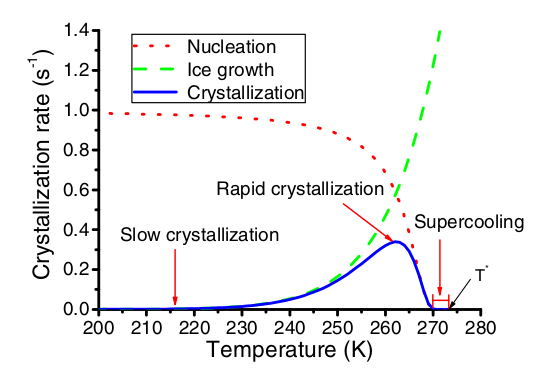
\includegraphics[width=0.6\textwidth]{crystallization_rate.png}
	\caption{Crystallization rate versus temperature.}	
	\label{fig:boat2}
\end{figure} 
Finally, the coefficient $C_f$ that appears on Equations \ref{3.2} and \ref{3.3} as commented above, is defined for the Lee model as:
\begin{equation}
\label{2.28}
C_f=J_{\mathrm{hom}} \cdot V_{l}
\end{equation}
where $V_{l}$ is the volume of water in each cell.
\subsection{Interphase porosity models}
Interphase porosity models add an aritificial momentum source over the interface between phases to compute the sink of velocity in the solidified region. Therefore, influencing the behavior of the physics during the process of solidification or melting.
\newline
The model implemented in OpenFOAM is \textit{Voller Prakash method} and it defines the source terms, \textit{$S_y$} and \textit{$S_z$} such that when along the fluid domain these terms take on a value of zero, the momentum equations are driven by the actual values of the velocities. On the other side, when it comes to treat the mushy region (i.e. porous region), the value of these source terms dominate convective, diffusive and transient terms and the momentum equation tends to approximate de Darcy law.
\newline
The two source terms as specified above,
\begin{equation}
\left\{\begin{array}{l}
S_{y}=-A v \\
S_{z}=-A w
\end{array}\right.
\label{2.29}
\end{equation}
Then, to specify a term for the function A, it is used the \textit{Carman-Koseny equation}, which is derived from the Darcy law. The former expresses the gradient for the pressure as a combination of the velocity, \textbf{u}, and the porosity, $\lambda$. The coefficient \textit{C} depends on the morphology of the medium.
\begin{equation}
gradP=-\left(\frac{C(1-\lambda)^{2}}{\lambda^{3}}\right) \mathbf{u}
\label{2.30}
\end{equation}
To avoid division by zero, \textit{q} is added to the equations shown 
\begin{equation}
A=-\left(\frac{C(1-\lambda)^{2}}{\lambda^{3}+q}\right)
\label{2.31}
\end{equation}
The source terms $S_{y}$ and $S_{z}$ are added in the Eq. \ref{3.32} and \ref{3.33}. The source term $S_{b}$ corresponds to the body forces of the fluid and will be discused later on this thesis.
\begin{equation}
	\begin{aligned}
		\frac{\partial(\rho v)}{\partial t}+\operatorname{div}(\rho \mathbf{u} v)=\operatorname{div}(\mu \operatorname{grad} v)-\frac{\partial P}{\partial y}+S_{y} 
	\end{aligned}
	\label{2.32}
\end{equation}
\begin{equation}
	\begin{aligned}
		\frac{\partial(\rho w)}{\partial t}+\operatorname{div}(\rho \mathbf{u} w)=\operatorname{div}(\mu \operatorname{grad} w)-\frac{\partial P}{\partial z}+S_{z}+S_{b}
	\end{aligned}
	\label{2.33}
\end{equation}
\subsubsection{Surface tension model}
The surface tension is only specified on a phase pair basis. In this version of OpenFOAM, it is present a constant model for a given $\sigma$.




 
% Chapter 1

\chapter{Numerical Simulation of Solidification Process} % Main chapter title

\label{Chapter3} % For referencing the chapter elsewhere, use \ref{Chapter1} 
\section{OpenFOAM. General Aspects}

\setlength{\parindent}{0.5cm} OpenFOAM is a free open-source software written in C++ and mainly conceived to perform computational fluid dynamics (CFD) simulations based on a finite volume discretization (FVM). 

\subsection{The finite volume method}

\setlength{\parindent}{0.5cm} Fluid equations usually take the form of non-linear partial differential equations and so, most of time, no analytical solution can be derived from them. In that context, different numerical techniques are employed to reach an approximation of the solution to these problems. These methods require a discretization of the domain in which the solution is going to be calculated. As aforementioned, OpenFOAM uses the finite volume method, which is, indeed, one of the most widely techniques used in computational fluid dynamics, and the one used in this thesis.

\noindent This technique turns the partial differential equations, which at their turn represent conservation laws over differential volumes, into discrete algebraic equations over finite volumes. Similarly to the finite element method, the FVM also needs a discretization of the geometric domain but in this numerical method, the elements used to integrate the algebraic equations representing the conservation partial differential equations are finite volumes.

\noindent Some of the terms in the conservation equation are converted into face fluxes and evaluated in the discretized finite volumes. These face fluxes are strictly conservative. This is that the flux entering the volume is equal to the flux leaving the adjacent volume. This property makes the finite volume method the preferred technique for CFD \cite{moukalled_mangani_darwish_2016}. 

\subsubsection*{Geometric domain discretization}

\setlength{\parindent}{0.5cm} The intrinsic properties of the finite volume method need the computational domain to be discretized in volume cells, known as control volumes (CV). Each one of these volumes has a centroid or computational point in which the solution is obtained. 

\noindent Alongside with this idea, OpenFOAM follows a cell-centered approach in which the unknowns are defined at the center of these volumes or cells. The value of these are computed as an average value of the variable in that cell.

\noindent Moreover, the control volume is defined by the neighbours. This is, in the case the volume has an adjacent neighbour, an internal face is delimiting the separation of both. On the other hand, if the volume is not sharing a face with a neighour volume, the face is considered to be a boundary.

\subsubsection*{Discretization of the fluid dynamic's equations}

\setlength{\parindent}{0.5cm} The continuity equation, the Navier-Stokes equations and, the heat equation stated in section 2 can be stated in a more general form under the formulation of the Reynolds transport theorem:
\begin{equation}
	\underbrace{\int_{V_{P}} \frac{\partial \rho \phi}{\partial t} d V}_{\text {Temporal term }}+\underbrace{\int_{V_{P}} \nabla \cdot(\rho \vec{u} \phi) d V}_{\text {Convective term }}=\underbrace{\int_{V_{P}} \nabla \cdot\left(\rho \Gamma_{\phi} \nabla \phi\right) d V}_{\text {Diffusive term }}+\underbrace{\int_{V_{P}} S_{\phi} d V}_{\text {Source term }}
	\label{3.1}
\end{equation}
where $V_{P}$ is the control volume cell, $\phi$ may be any scalar or vectorial variable of the continuum, $\Gamma_{\phi}$ is the diffusivity of the variable and $S_{\phi}$ is a source term. 

\noindent In order to recover the continuity, momentum and energy equations, the parameters shown in table \ref{3.1tab} need to be shaped in the transport equation.
\begin{table}[h!]
	\begin{tabular}{@{}lllll@{}}
		\toprule[1pt]
		\textbf{Equation} & \textbf{$\phi$} & \textbf{$\Gamma_{\phi}$} & \textbf{$S_{\phi}$}  \\ \midrule[2pt]
		\textbf{Continuity} & 1 & 0 & 0  \\
		\textbf{Momentum} & $\vec{u}u$ & $\nu$ & -$\nabla p$\\
		\textbf{Energy} & $C_{p}T$ & $\kappa$ & 0\\ \bottomrule[1pt]		
	\end{tabular}
	\centering
	\caption{Parameters to recover continuity, momentum and energy equations.}	
	\label{3.1tab}
\end{table}
\newline
The fluid variable is defined as a ratio of itself integrated along the volume cell. Thus, it yelds the following form,
\begin{equation}
	\phi=\phi_{P}=\frac{1}{V_{p}} \int_{V_{P}} \phi(x) d V
	\label{3.2}
\end{equation}
Therefore, a complete discretization of the previous terms is needed to solve the physics regarding a general fluid dynamics problem.
\subsection{OpenFOAM functioning}
\setlength{\parindent}{0.5cm} In this first section, a brief introduction on the structure and functioning of the OpenFOAM software is given.

\noindent In the folder structure tree shown in Fig. \ref{3.1fig},  it is shown a typical case setup for a phase change problem using \textit{icoReactingMultiphaseFoam} solver.

\begin{figure}[h!]
	\centering
	\scalebox{0.75}{
	\begin{forest}
		for tree={
			font=\ttfamily,
			grow'=0,
			child anchor=west,
			parent anchor=south,
			anchor=west,
			calign=first,
			edge path={
				\noexpand\path [draw, \forestoption{edge}]
				(!u.south west) +(7.5pt,0) |- node[fill,inner sep=1.25pt] {} (.child anchor)\forestoption{edge label};
			},
			before typesetting nodes={
				if n=1
				{insert before={[,phantom]}}
				{}
			},
			fit=band,
			before computing xy={l=15pt},
		}
		[phaseChangeCase
		[0*
		[alpha.liquid]
		[alpha.solid]
		[p]
		[$p_{rgh}$]
		[T]
		[U]
		]
		[constant*
		[g]
		[phaseProperties]
		[thermophysicalProperties.liquid]
		[thermophysicalProperties.solid]
		[turbulenceProperties]
		[polyMesh]
		]
		[system*
		[blockMeshDict]
		[controlDict]
		[decomposeParDict]
		[fvSchemes]
		[fvSolution]
		]
		]
	\end{forest}}
	\caption{General structure of an OpenFOAM case.}
	\label{3.1fig}
\end{figure}

\subsubsection{Boundary Conditions Directory}

\setlength{\parindent}{0.5cm} The "0" directory gathers all the boundary conditions at time zero and the initial conditions to set up the case. As the simulation starts running, the information of these fields is saved in folders at every timestep.

\subsubsection{Constant Properties Directory}

\setlength{\parindent}{0.5cm} The "constant" directory contains all the information typically regarding the physical properties which are kept constant through the simulation. Moreover, once the dictionary \textit{blockMeshDict} is run, OpenFOAM creates a folder called \textit{polyMesh} containing all the information relevant to the mesh (points, faces,...). 

\subsubsection{System Directory}
\setlength{\parindent}{0.5cm} This folder contains the files required by the control of the solver and the solution itself. The most common files are:
\begin{itemize}
	\item \textbf{blockMeshDict:} in this file the parameters required to build up the computational domain, the mesh and the boundaries are found. The command \textbf{blockMesh} executes this dictionary creating the \textit{polyMesh} folder commented above.
	\item \textbf{controlDict:} Time parameters associated to the computation are set in this file. 
	\item \textbf{decomposeParDict:} In the realization of this thesis, the help of parallel computing is required. Thus, in this file, parameters regarding the decomposition of the mesh are configured. It is executed by means of the \textbf{decomposePar} appliation implicit in OF. The mesh is afterwards reconstructed by using \textbf{reconstructPar} 
	\item \textbf{fvSchemes:} Schemes selected for the discretization of the derivative terms are defined. Among others, time schemes, gradient schemes, laplacian schemes, divergent schemes, interpolation schemes can be declared here.
	\item \textbf{fvSolution:} contains sub-dictionaries used to control the solvers and the solution algorithms. It also allows the definition of the fields resolution.
\end{itemize}
\clearpage
\section{Solidification process. Methodology}

\setlength{\parindent}{0.5cm} A convection solver is used to represent the flow behavior generated by the density difference due to existing temperature gradients whithin the volume of control. A polynomic water density is implemented in the native OpenFOAM solver and compared with the standard Boussinesq approximation. Besides, a proposed buoyancy term by Bourdillon \cite{bourdillon_2016} is added in the computation of the momentum equation. The current model is validated against numerical results from the literature. The solution of this convection solver is later used as initial conditions, before solidification phenomena plays a role.

\noindent For the solidification phenomena representation, the aforementioned Enthalpy-porosity technique and Lee model based on the \textit{Classical Nucleation theoy} are implemented within a multi-phase native solver. These methods are compared against \cite{bourdillon_2016}, Kowalesky et al. \cite{kowalewski_rebow_1999}, whose simulations rely on the enthalpy method and, Chen et al. \cite{chen_lee_1998}. A final remark on the \textit{classic Stefan problem} is done. 

\newpage
\section{OpenFOAM: BuoyantBoussinesqPimpleFOAM. Natural Convection solver}

\setlength{\parindent}{0.5cm} In a natural convection environment, the motion of the fluid is mainly driven by the density difference within the fluid volume of control. At its turn, the differences in the density, responsible for buoyancy forces, are generated by the existing temperature gradients. Within a physical context, the fluid near a hot heat source gets warmed up and, as a result, it becomes less dense moving up inside a domain. Consequently, the fluid in contact of the cold heat source is pushed from its zone to replace the hot fluid location. At this point, the cycle starts again repeating this phyisical phenomena.

\subsection{Case Description}
\setlength{\parindent}{0.5cm} Within the context of natural convection, the current case aims to develop a comprehensive state of the capabilities that OpenFoam solvers bring to solve this phenomena. To reach the objective, and on purpose of controlling the physics generated on the simulation, a regular squared geometry of 0.038 \textit{mm} side length is created:

\begin{figure}[h!]
	\centering
	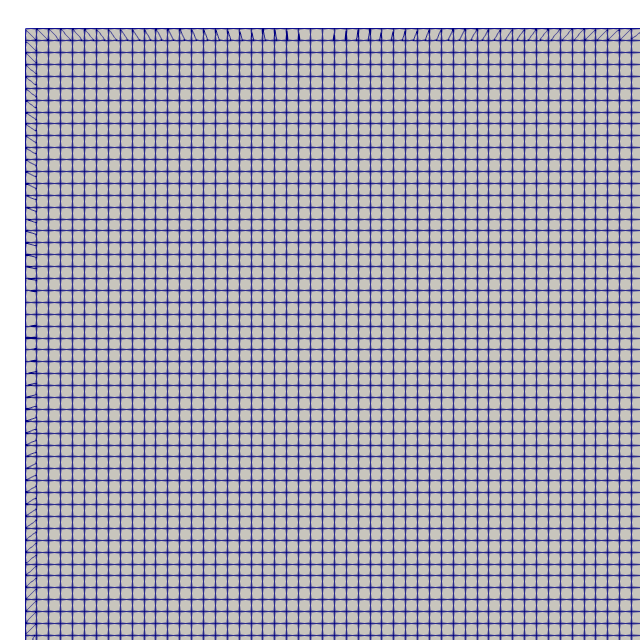
\includegraphics[width=.35\linewidth]{mesh_cavity.png}	
	\caption{Zoom of the computational mesh for the cavity.}
	\label{3.2fig}
\end{figure} 
The mesh is structured and consists of 1971212 nodes.

\subsection{Hypotheses And Assumptions}

\setlength{\parindent}{0.5cm} To carry out the current problem, a series of assumptions are taken into account in order to simplify the solving of the fluid equations involved.

\textbf{Laminar regime:} The Reynolds number, computed from the maximum velocity is not high enough to consider turbulent effects. 

\textbf{Convective heat transfer:} To determine whether the heat transfer is assumed to be convective, the Prandtl number and the Rayleigh number should be assessed.

\noindent The Prandtl number, as the relation between the viscosity and the thermal conductivity of a fluid or, in other words, the correlation between momentum transport and thermal transport capacity is calculated as:
\begin{equation}
	\operatorname{Pr}=\frac{v}{\alpha}=\frac{\mu}{\rho \alpha}=\frac{\mu c_{p}}{\lambda}=\frac{\text { momentum transport }}{\text { heat transport }}
	\label{3.3}
\end{equation}
where $\mu$ is the dynamic viscosity, $c_{p}$ is the specific heat and $\lambda$ is the thermal conductivity.

\noindent Thus, a small Prandtl number are owned by free-flowing flows with high thermal conductivitiy.

\noindent On the other hand, the Rayleigh number is referred to the time scale relation between the diffusive and the convective thermal transports. It is thus used to determine wheter the buoyancy-driven natural convection plays an important role in the heat transfer. The dimensionless number is assessed in this context by this form:
\begin{equation}
	\mathrm{Ra}_{x}=\frac{g \cdot \beta}{\nu \cdot \alpha} \cdot\left(T_{s}-T_{\mathrm{inf}}\right) \cdot x^{3}
	\label{3.4}
\end{equation}
Being \textit{g}, the gravity, \textit{$\beta$}, the coefficient of thermal expansion, \textit{$\nu$}, the kinematic viscosity, \textit{$\alpha$}, the thermal diffusivity, and \textit{$T_{s}$} and \textit{$T_{\mathrm{inf}}$}, the temperature on the wall surface and the temperature of the fluid far from the wall accordingly.

\noindent In the current case-scenario, a Prandtl close to 7 and a Rayleigh of 2517629 determine a convective heat transfer. The values used to estimate the Rayleigh number calculation are: $\beta = 6.734e-5 K^{-1}$, $\nu = 1.003e-6 m^{2}.s^{-1}$, $\alpha = 1.435e-7 m^{2}.s^{-1}$, $T_{s} = 283 K$, $T_{inf} = 273 K$ and $x = 0.038 m$. The values used for the laminar Prandtl number calculation are: $\mu = 0.001003 Kg.m^{-1}.s^{-1}$, $\lambda = 0.6 W.m^{-1}.K^{-1}$ and $C_{p}=4182 J.Kg.K^{-1}$.

\textbf{Newtonian fluid:} The viscosity of the fluid is assumed to be constant.

\textbf{Thermophysical properties:} specific heat, \textit{$C_p$}, the thermal expansion coefficient, \textit{$\beta$}, thermal conductivity, \textit{$\kappa$}, kinematic viscosity, \textit{$\nu$} are assumed to be non-dependent of temperature. However, the density will be dependent of temperature so as it plays an important role in the buoyancy effects through the later explained in this section.

\noindent The conservative equations used to describe the motion of the fluid along time and space are described next.

\subsection{Governing Equations}

\setlength{\parindent}{0.5cm} In this section, the governing equations for the used solver are described first.

The conservation of mass states that the mass flowing into the volume of control (CV) must be equal to the mass flowing out of such volume. 
\begin{equation}
	\frac{\partial v}{\partial y}+\frac{\partial w}{\partial z}=0
	\label{3.5}
\end{equation}

\subsubsection{Momentum Equation}

\setlength{\parindent}{0.5cm} Throughout the CV the momentum of the fluid flow is preserved and here below it is expressed for the y-direction and z-direction.
\begin{equation}
	\begin{aligned}
		\frac{\partial(\rho v)}{\partial t}+\operatorname{div}(\rho \mathbf{u} v)=\operatorname{div}(\mu \operatorname{grad} v)-\frac{\partial P}{\partial y}
	\end{aligned}
	\label{3.6}
\end{equation}
\begin{equation}
	\begin{aligned}
		\frac{\partial(\rho w)}{\partial t}+\operatorname{div}(\rho \mathbf{u} w)=\operatorname{div}(\mu \operatorname{grad} w)-\frac{\partial P}{\partial z}+S_{b}
	\end{aligned}
	\label{3.7}
\end{equation}
where in the case of the \textit{Boussinesq approximation} where the density variation is linear:
\begin{equation}
	S_{b} = g\cdot\rho_{r}[1-\beta(T-T_{r})]
	\label{3.8}
\end{equation}
in the case of the implemented polynomial density which accounts for the inversion point as in \cite{bourdillon_2016}:
\begin{equation}
	S_{b} = g\cdot[\rho_{r}-\rho(T)]
	\label{3.9}
\end{equation}
where the polynomial expression from $\rho$ is:
\begin{equation}
	\begin{aligned}
		\rho(T) &=999.840281167108+0.0673268037314653 \times T \\
		&-0.00894484552601798 \times T^{2} \\
		&+8.78462866500416 .10^{-5} \times T^{3} 
		-6.62139792627547 .10^{-7} \times T^{4}
	\end{aligned}
	\label{3.10}
\end{equation}
As it will be pointed out later, the native solver uses the Boussinesq approximation to account for the buoyancy effects. However, this linear assumption is only valid as the density variations meet:
\begin{equation}
	\frac{\Delta \rho}{\rho_{r}}<<1
	\label{3.11}
\end{equation}
Therefore, to account for the inversion points present during the freezing process, a density variation like the described in Eq. \ref{3.10} is implemented in the solver.

\subsubsection{Temperature Equation}
\setlength{\parindent}{0.5cm} The temperature equation representing the convection phenomena yields as:
\begin{equation}
	\begin{aligned}
	\frac{\partial T}{\partial t}+ \frac{\partial (u_{j} T)}{\partial x_{j}}=\frac{\partial}{\partial x_{j}}\left(\gamma \frac{\partial T}{\partial x_{j}}\right)
	\end{aligned}
	\label{3.12}
\end{equation}

where the thermal diffusivity, $\gamma$, is defined as:
\begin{equation}
	\gamma=\frac{\lambda}{\rho_{r} c_{p}}
	\label{3.13}
\end{equation}

All these equations are regarded by the solver \textit{buoyantBoussinesqPimpleFoam}.

\subsection{Solver descripton. Control Loop}

\setlength{\parindent}{0.5cm} The \textit{buoyantBoussinesqPimpleFoam} is a solver used to solve non-steady buoyancy driven fluids by using the Boussinesq approximation as a coupling between density and temperature fields. It considers the fluid as incompressible and uses the PIMPLE algorithm for the pressure-velocity coupling. The flowchart of the integration procedure for the presented solvers \textit{buoyantBoussinesqPimpleFoam} and \textit{icoReactingMultiphaseinterFoam} is presented below:

\tikzstyle{decision} = [diamond, draw, fill=blue!20,
text width=4.5em, text badly centered, node distance=2.5cm, inner sep=0pt]
\tikzstyle{block} = [rectangle, draw, fill=blue!20,
text width=5em, text centered, rounded corners, minimum height=4em]
\tikzstyle{line} = [draw, very thick, color=black!50, -latex']
\tikzstyle{cloud} = [draw, ellipse,fill=red!20, node distance=2.5cm,
minimum height=2em]

\begin{figure}[h!]
	\centering
	\begin{tikzpicture}[scale=1.5, node distance = 2cm, auto]
	% Place nodes
	\node [block] (init) {Velocity predictor};
	\node [block, below of=init] (identify) {Temperature Equation};
	\node [block, below of=identify] (evaluate) {Pressure Equation};
	\node [block, below of=evaluate] (update) {Velocity Corrector};
	\node [block, left of=evaluate, node distance=3cm] (update1) {PIMPLE LOOP};
	\node [block, right of=evaluate, node distance=3cm] (update2) {PISO LOOP};
	\node [decision, below of=update] (decide) {Residuals satisfied?};
	\node [block, below of=decide, node distance=2.5cm] (stop) {stop};
	% Draw edges
	\path [line] (init) -- (identify);
	\path [line] (identify) -- (evaluate);
	\path [line] (evaluate) -- (update);
	\path [line] (update) -- (decide);
	\path [line] (decide) -| node [near start, color=black] {no} (update1);
	\path [line] (update1) |- (init);
	\path [line] (update) -| node [near start, color=black] {} (update2);
	\path [line] (update2) -- (evaluate);	
	\path [line] (decide) -- node [, color=black] {yes}(stop);
	
	\end{tikzpicture}
	\label{3.3fig}
	\caption{Flowchart of integration procedure. \textit{buoyantBoussinesqPimpleFoam}}
\end{figure}

\subsection{Code implementations}

\setlength{\parindent}{0.5cm} As described in the \textit{Governing equations} section, the need for a polynomial density expression and a variation of the momentum source terms devoted to reflect the buoyancy effects is derived.

\noindent To do so, a new equation of state is implemented within the OpenFoam framework. Now and, in order to take into account this bouyancy forces, the pressure equation is studied. This is beacause in the context of a pressure-velocity corrector scheme, and in the case of ensuring stability and simplifying the boundary conditions definition, the modified pressure, \textit{$p_{rgh}$}, within the pressure equation implementation, is the term that accounts for the gravity terms.

\noindent Here, it is presented a general form of a momentum equation with the continuity equation corresponding to a incompressible flow.  
\begin{equation}
	\left\{\begin{array}{l}
	\frac{\partial (\rho \textbf{v})}{\partial t}+\nabla \cdot(\rho \textbf{v} \otimes \textbf{v})=-\nabla p+ \nabla \cdot(\mu (\nabla \textbf{v}+\nabla \textbf{v}^{T})) \\
	\nabla \cdot \textbf{v}=0
	\end{array}\right.
	\label{3.14}
\end{equation}
From this general equation, it will be given the term $H(\textbf{u})$, as later on will be needed for the pressure equation calculation.

\noindent Therefore, this term comes from considering the linearization of the advective term under the assumption of small Courant numbers (Co < 1). Leading the term $\textbf{v}^{0}\cong\textbf{v}$. 
\begin{equation}
	\begin{aligned}
	\int_{\Omega} \nabla \cdot\left(\textbf{v} \otimes \textbf{v}^{0}\right) d \Omega & \cong \sum_{f} \textbf{v}_{f} \textbf{v}_{f}^{0} \cdot \textbf{S}_{f} \\
	&=\sum_{f} F^{0} \textbf{v}_{f} \\
	&=a_{P} \textbf{v}+\sum_{f} a_{N} \textbf{v}_{N}
	\end{aligned}
	\label{3.15}
\end{equation}

\begin{equation}
	a_{P} \textbf{v}_{P}=\textbf{H}(\textbf{v})-\nabla p
	\label{3.16}
\end{equation}
\begin{equation}
	\textbf{H}(\textbf{v})=\underbrace{-\sum_{f} a_{N} \textbf{v}_{N}}_{\text {Diagonal term }}+\underbrace{\frac{\textbf{v}^{0}}{\Delta t}}_{\text {Off-diagonal term }}
	\label{3.17}
\end{equation}
where $\textbf{v}^{0}$ is the velocity at previous time-step and $F^{0}$ is the face flux at the previous time-step.

\noindent In addition, by discretizing the continuity equation, it is possible to get the final form of the pressure equation.

\noindent So as to give stability to the solution and to simplify the boundary conditions definition as described in Berberovic et al. \cite{berberovic_van_hinsberg_jakirlic_roisman_tropea_2009}, a modified pressure is defined as,
\begin{equation}
	p_{r g h}=p-\rho_{r} \textbf{g} \cdot \textbf{x} + \rho(T) \textbf{g} \cdot \textbf{x}
	\label{3.18}
\end{equation}
being, the pressure gradient the next expression,
\begin{equation}
	-\nabla p+\rho_{r} \textbf{g}=-\nabla p_{r g h}-\textbf{g} \cdot \textbf{x} \nabla \rho_{r} + \textbf{g} \cdot \textbf{x} \nabla \rho(T) + \rho(T) \textbf{g}
	\label{3.19}
\end{equation}
and rearranging terms, 
\begin{equation}
	-\nabla p+\rho_{r} \textbf{g} + \textbf{g} \cdot \textbf{x} \nabla \rho_{r} - \textbf{g} \cdot \textbf{x} \nabla \rho(T) - \rho(T) \textbf{g}=-\nabla p_{r g h}
	\label{3.20}
\end{equation}
If one tries to describe the discretized pressure equation in \textit{buoyantBoussinesqPimpleFoam}, there is a first term called \textbf{phig}, which is,
\begin{equation}
	\Phi_{f}^{\nu+1}=\Phi_{u}^{\nu+1} - \left[(\textbf{g} \cdot \textbf{x})_{f}\left(\nabla \rho_{r}{ }^{n+1}\right)_{f}+(\textbf{g} \cdot \textbf{x})_{f}\left(\nabla \rho(T){ }^{n+1}\right)_{f}\right]\frac{\left|\textbf{S}_{f}\right|}{\left(a_{P}\right)_{f}}
	\label{3.21}
\end{equation}
This term is edited in the code so as it handles the new expression for the buoyancy effects as regarded by Bourdillon, \cite{bourdillon_2016}.

A face flux calculated by the term \textbf{H}(\textbf{v}), appearing in equation \ref{3.17}
\begin{equation}
	\Phi_{u}^{\nu+1}=\Phi_{f}^{\nu+1} + \left(\frac{H\left(\textbf{v}^{\nu}\right)}{a_{P}}\right)_{f} \cdot \textbf{S}_{f}+\left(\frac{1}{a_{P}}\right)_{f}\operatorname{ddt} \operatorname{PhiCorr}\left(\textbf{v}^{\nu}, \Phi^{\nu}\right)
	\label{3.22}
\end{equation}
where $\operatorname{ddt} \operatorname{PhiCorr}$ is a flux adjustment due to the time-step. This is resolved by applying a \textit{Rhie-Chow interpolation} \cite{rhie_chow_1983}, the next term in the pressure equation, \textbf{phiHbyA}, reads as,
\begin{equation}
	\Phi_{f}^{\nu+1}=\Phi_{f}^{\nu+1}-\left[\left(\frac{1}{a_{P}}\right)_{f}\left(\nabla p_{r g h}\right)_{f}\right] \cdot \textbf{S}_{f}
	\label{3.23}
\end{equation}
The \textbf{$p_{rgh}$} term is thus assembled as,
\begin{equation}
	\sum_{f}\left[\left(\frac{1}{a_{P}}\right)_{f}\left(\nabla p_{r g h}^{\nu+1}\right)_{f}\right] \cdot \textbf{S}_{f}=\sum_{f} \Phi^{\nu+1}
	\label{3.24}
\end{equation}
The flux, \textit{$\phi$}, is adjusted by the \textbf{$p_{rgh}$} term yielding the following expression,
\begin{equation}
	\Phi_{f}^{\nu+1}=\Phi_{f}^{\nu+1}-\left[\left(\frac{1}{a_{P}}\right)_{f}\left(\nabla p_{r g h}\right)_{f}\right] \cdot \textbf{S}_{f}
	\label{3.25}
\end{equation}
\begin{equation}
	\begin{aligned}
		\Phi_{f}^{\nu+1}=&\Phi_{f}^{\nu+1}+\biggl[\left(\frac{1}{a_{P}}\right)_{f}\biggl[(-\nabla p)_{f}+ (\textbf{g} \cdot \textbf{x})_{f}\left(\nabla \rho_{r}{ }^{n+1}\right)_{f}-(\textbf{g} \cdot \textbf{x})_{f}\left(\nabla \rho(T){ }^{n+1}\right)_{f}\\
		&+ (\rho_{r}{ }^{n+1} \textbf{g})_{f}-(\rho(T){ }^{n+1} \textbf{g})_{f} \biggr]\biggr] \cdot \textbf{S}_{f}
	\end{aligned}
	\label{3.26}
\end{equation}
Finally, the velocity calculated at the center of the volume reads as,
\begin{equation}
	\textbf{v}^{\nu+1}=\textbf{v}^{\nu+1} +\frac{1}{a_{P}}\mathcal{R}\left[\left(\Phi^{\nu+1} f-\Phi_{u}^{\nu+1} f\right)\left(a_{P}\right)_{f}\right]
	\label{3.27}
\end{equation}
where $\mathcal{R}$ is an operator used to recover cell-centered fields from fields given as fluxes at faces.
Then, the static pressure, \textit{p}, is reconstructed from \textit{$p_{rgh}$}, leading the expression,

\begin{equation}
	p = p_{r g h} + (\rho_{r}-\rho(T))\textbf{g}\cdot \textbf{x}
	\label{3.28}
\end{equation}
 
\subsection{Case Setup}

\setlength{\parindent}{0.5cm} Once the implementation is done, a first case is studied with the existing solver, \textit{buoyantBoussinesqPimpleFoam}. Later, the same case is settled with the new implementations.
The boundary conditions, thermophysical properties and some other solver parameters are described along the following subsections.
\newline
As commented before, all studies are calculated on a computational domain of \textit{38mm x 38mm}. 
\begin{figure}[h]
	\label{3.4fig}	\centering	
	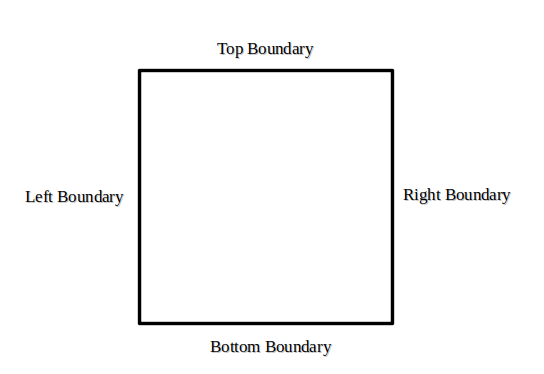
\includegraphics[width=0.6\textwidth]{domain.png}
	\caption{Setting of cavity computational domain.}
\end{figure} 

\subsubsection*{Boundary conditions}
\setlength{\parindent}{0.5cm} Five boundaries are defined in the current case:
\newline
\textbf{Left:} is considered a wall with a fixed value of temperature. This is the hot wall. No velocity is prescribed.
\newline
\textbf{Right:} considered to be the cold wall with a fixed temperature. No velocity is prescribed.
\newline
\textbf{Top:} this is considered the top wall and it is adiabatic, thus, no heat transfer is assumed and zero gradient is applied. No velocity is applied.
\newline 
\textbf{Bottom:} This shares similar conditions as the top wall.
\newline
\textbf{frontAndBack:} this uses a symmetry plane condition in the z direction since the problem is considered to be 2-dimensional. For such boundary type, no more conditions need to be prescribed.
\begin{table}[h!]
	\begin{tabular}{@{}lllll@{}}
		\toprule[1pt]
		\textbf{Boundary} & \textbf{Conditions}  \\ \midrule[2pt]
		Left & $T_{l}=283, v_{l} = 0   $  \\
		Right & $T_{r}=273, v_{r} = 0 $ \\
		Top & $\frac{\partial T_{u}}{\partial n} = 0, v_{u} = 0$  \\
		Bottom & $\frac{\partial T_{b}}{\partial n} = 0, v_{b} = 0$  \\ \bottomrule[1pt]		
	\end{tabular}
	\centering
	\caption{Boundary conditions for natural convection case.}	
	\label{3.2tab}
\end{table}
\newline

\subsubsection*{Thermophysical properties}
The thermophysical properties for the natural convection calculation are described in \ref{3.3tab}. 
\begin{table}[h!]
	\begin{tabular}{@{}lllll@{}}
		\toprule[1pt]
		\textbf{Water properties} & \textbf{Symbol} & \textbf{Values} & \textbf{Units} &  \\ \midrule[2pt]
		Density & $\rho_r$ & 999.8 & $kg.m^{-3}$ \\
		Dynamic viscosity & $\mu$ & 0.001003 & $kg.m^{-1}.s^{-1}$ \\
		Thermal conductivity & $\lambda$ & 0.6 & $W.m^{-1}.K^{-1}$ \\
		Heat capacity & $C_p$ & 4182 & $J.kg.K^{-1}$ \\		 
		Gravitational acceleration & $g$ &  9.81  & $m.s^{-2}$ \\
		Thermal diffusivity & $\gamma$ &  1.435e-7  & $m^{2}.s^{-1}$ \\		
		Thermal expansion coefficient & $\beta$ &  6.734e-5  & $K^{-1}$ \\	
		Laminar Prandtl number & $P_r$ &  6.99  & - \\
		Reference temperature & $T_r$ &  6.734e-5  & $K$ \\ \bottomrule[1pt]		
	\end{tabular}
	\centering
	\caption{Water properties for natural convection.}	
	\label{3.3tab}
\end{table}
\newline
Here below are presented the discretization schemes used for the terms appearing on the equations involved in the calculation. For more information on the used ones, refer to \cite{openfoamuserguide:cfddirect}.
\begin{table}[h!]
	\begin{adjustbox}{width=1\textwidth}
		\small	
		\begin{tabular}{@{}lllll@{}}
			\toprule[1pt]
			\textbf{Modeling Term} & \textbf{Keyword} & \textbf{Scheme} & \textbf{Remarks} &  \\ \midrule[2pt]
			Time derivatives & ddtSchemes    &  Euler  & First order, bounded, implicit \\
			Divergence term    & divSchemes   &    & Second order, unbounded \\
			Gradient term    & gradSchemes    &  Gauss linear  & Second order, unbounded \\
			Laplacian term   &  laplacianSchemes    &  Gauss linear orthogonal  & Second order \\		 
			Grad. normal to cell face & snGradSchemes    &  orthogonal  &  Second order\\ 
			Point to point interpolation&    			   interpolationSchemes    & linear   & Central differencing \\ \bottomrule[1pt]		
		\end{tabular}
	\end{adjustbox}
	\centering
	\caption{Discretization schemes.}	
	\label{3.4tab}
\end{table}
\clearpage
The equation solvers are shown in \ref{3.5tab}. 
\begin{table}[h!]
	\begin{tabular}{@{}lllll@{}}
		\toprule[1pt]
		\textbf{Equation} & \textbf{Linear Solver} & \textbf{Smoother/Preconditioner} & \textbf{Tolerance} &  \\ \midrule[2pt]
		Pressure correction equation & PCG & DIC & 1e-8 \\
		Momentum equation & PBiCGStab & DILU  & 1e-6 \\
		Temperature equation & PBiCGStab & DILU  & 1e-6 \\\bottomrule[1pt]		
	\end{tabular}
	\centering
	\caption{Solvers for the discretised equations.}	
	\label{3.5tab}
\end{table}
\newline
Table \ref{3.6tab} presents the parameters used for the inner and outter loops performed within the calculation.
\begin{table}[h!]
	\begin{tabular}{@{}lllll@{}}
		\toprule[1pt]
		\textbf{Parameter} & \textbf{Value} \\ \midrule[2pt]
%		nAlphaCorr & PCG & DIC &  \\
%		nAlphaSubCycles & smoothSolver & symGaussSeidel  &  \\
%		cAlpha & smoothSolver & symGaussSeidel  &  \\
		momentumPredictor &  no    &    &  \\		 
		nOuterCorrectors &  1   &    &  \\ 
		nNonOrthogonalCorrectors &  0   &    &  \\ 		
		nCorrectors & 2	&    &  \\ \bottomrule[1pt]		
	\end{tabular}
	\centering
	\caption{Parameters for the discretised equations.}	
	\label{3.6tab}
\end{table}

\clearpage
\subsection{Validation of Results and Conclusions}
For comparison purposes and so as to know the state of the art in the natural convection phenomena, a first analysis is performed using the convection solver provided by OpenFOAM. This solver is BuoyantBoussinesqPimpleFoam and it covers both laminar and turbulent unsteady heat transfer for single phase fluids using the Boussinesq approximation. Afterwards, the case is calculated with the new implementations described.
\begin{figure}[h!]
	\centering
	\begin{subfigure}{\linewidth}
	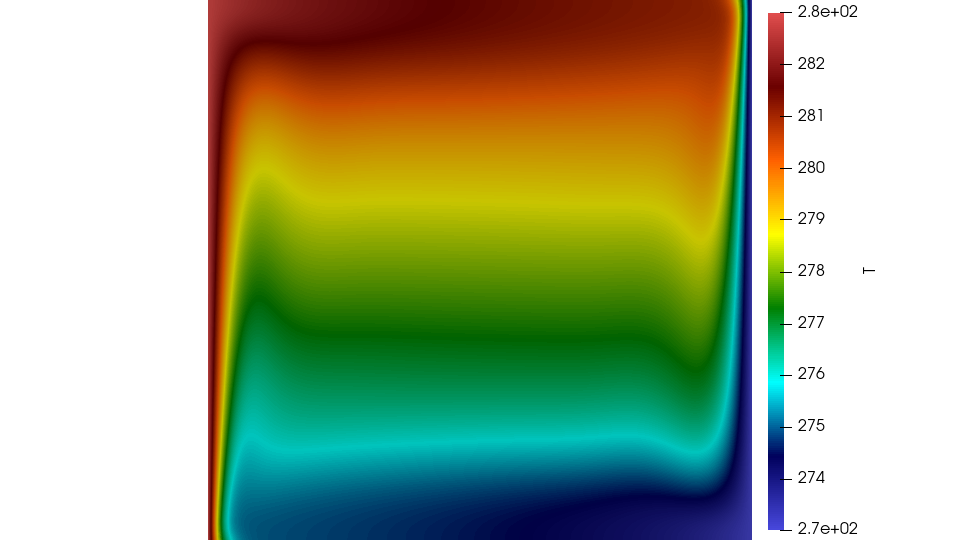
\includegraphics[width=.55\linewidth]{BBPF_T_1500s.png}\hfill
	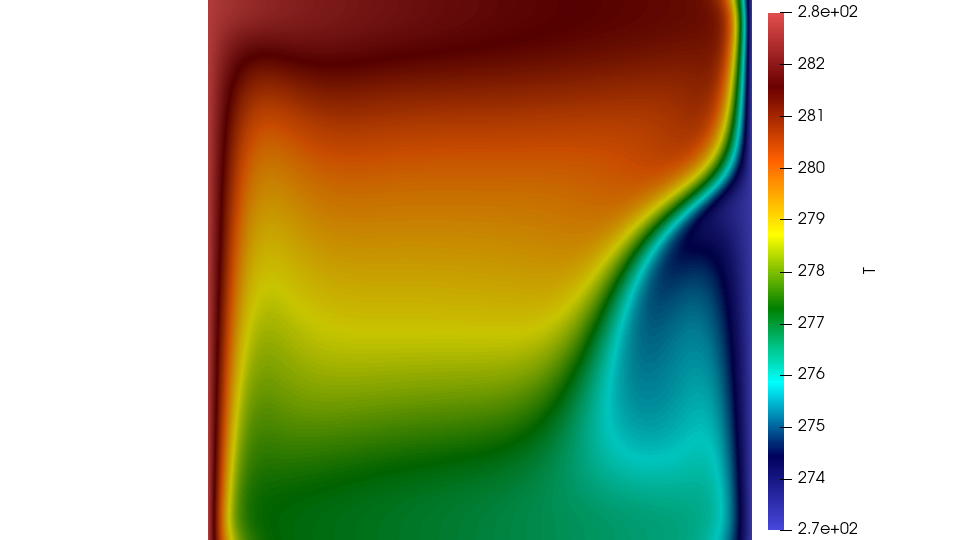
\includegraphics[width=.55\linewidth]{CF_T_1500s_comp.png}	
	\caption{Temperature magnitude comparison at t = 1500s. Left: BBPF. Right: mBBPF.}
	\label{3.5figa}
	\end{subfigure}\par\medskip
	\begin{subfigure}{\linewidth}
	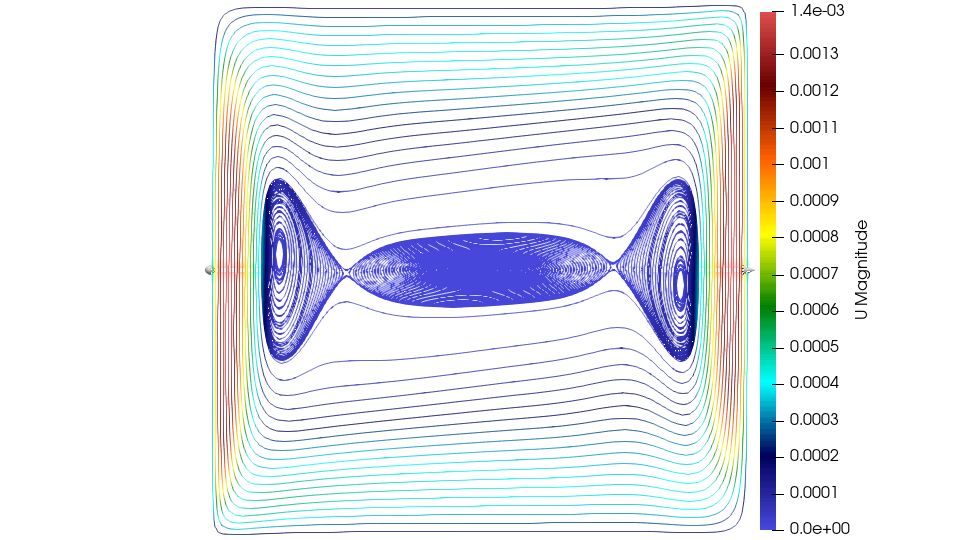
\includegraphics[width=.55\linewidth]{BBPF_U_1500s.png}\hfill
	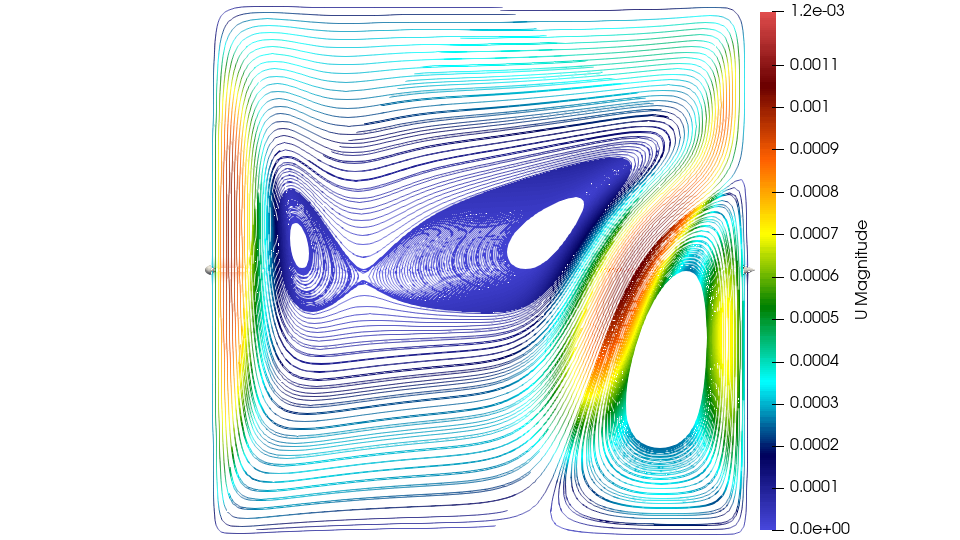
\includegraphics[width=.55\linewidth]{CF_U_1500s_comp.png}	
	\caption{Velocity magnitude comparison at t = 1500s. Left: BBPF. Right: mBBPF}
	\label{3.5figb}
	\end{subfigure}\par\medskip
	\caption{Comparison between BBPF* and mBBPF**}
	\label{3.5fig}
\end{figure}
\newline 
BBPF*: BuoyantBoussinesqPimpleFoam solver.
mBBPF**: myBuoyantBoussinesqPimpleFoam, natural convection modified solver.

\noindent The gravity terms of the temperature and velocity magnitude distributions shown in Fig. \ref{3.5fig} (left) are as expressed in Equation \ref{3.8}, $(S_{b} = g\cdot\rho_{r}[1-\beta(T-T_{r})])$. In addition, the equation of state used to describe the behavior of the liquid density variation is linear. On the other hand, the proposed gravity terms proposed by \cite{bourdillon_2016} and described in Equation \ref{3.9}, $(S_{b} = g\cdot[\rho_{r}-\rho(T)])$, besides of the polynomial density variation have depicted a non-linear pattern for the temperature and velocity magnitude distibutions. It is seen that small changes in the density, $0.171925 kg.m^-3$ in this case, Fig. \ref{rhodifffig}, may induce different patterns within the flow. 
\clearpage
\begin{figure}[h!]
	\centering
	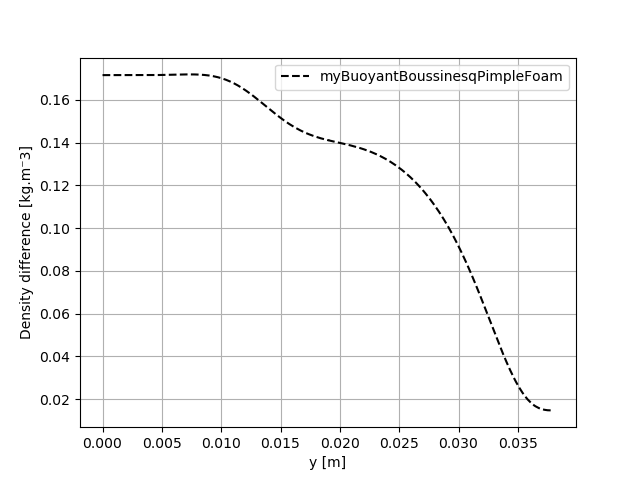
\includegraphics[width=.55\linewidth]{rhodiff_CF.png}\hfill
	\caption{Density differences between linear and polynomial expressions.}
	\label{rhodifffig}
\end{figure} 

\noindent The fact of achieving the description of the inversion point in the temperature distribution due to the density variation of the density will influence the growth of the ice layer in the phase change simulations.

\noindent Therefore, in order to compare consistently the obtained results with those of the literature, the following dimensionless values are pointed out:

\noindent Dimensionless values of temperature are described as:
\begin{equation}
	\tilde{T}=\frac{T-T_{\text {cold }}}{T_{\text {hot }}-T_{\text {cold }}}=\frac{T-273}{10}
	\label{3.29}
\end{equation}
Horizontal and vertical dimensionless positions along the x and y mid-planes:
\begin{equation}
	\tilde{x}=\frac{x}{\ell}=\frac{x}{38 \times 10^{-3}}
	\label{3.30}
\end{equation}
\begin{equation}
\tilde{y}=\frac{y}{\ell}=\frac{y}{38 \times 10^{-3}}
\label{3.34}
\end{equation}
Transversal and axial dimensionless velocities:
\begin{equation}
	\tilde{v}=\frac{v \ell}{\gamma}=\frac{v 38 \times 10^{-3}}{1.435 \times 10^{-7}}
	\label{3.31}
\end{equation}
\begin{equation}
	\tilde{u}=\frac{u \ell}{\gamma}=\frac{u 38 \times 10^{-3}}{1.435 \times 10^{-7}}
	\label{3.32}
\end{equation}

\clearpage
\noindent The presented dimensionless quantities obtained with the gravity related terms implemented in the convection solver are compared against the literature. Bourdillon et al. \cite{bourdillon_2016} used as a reference and guideline, worked out a solution using OpenFOAM and Kowalewski et al. \cite{kowalewski_rebow_1999} who in 1999 performed similar calculations using Fluent.

\noindent The results obtained with myBuoyantBoussinesqPimpleFoam, the natural convection modified solver, show acceptable agreement with the results found in the literature. The highest local differences are found in the V-velocity along the vertical direction, Fig. \ref{3.6ffig}. The relative error of the proposed numerical solution with respect to the one shown in Kowaleswki et al. remains below 16\%. Moreover, as it is observable, the temperature dimensionless, Fig. \ref{3.6bfig}, distribution and the U-velocity, Fig. \ref{3.6dfig}, plotted along the vertical mid-plane seem to be in short disaccordance with respect to the literature's solutions. This differences might be due to a small shift of the dimensionless magnitudes along that direction. However, in overall, the results nearly overlap the ones found in the bibliography.
\clearpage
\begin{figure}[h!]
	\begin{subfigure}{0.50\textwidth}
		\centering
		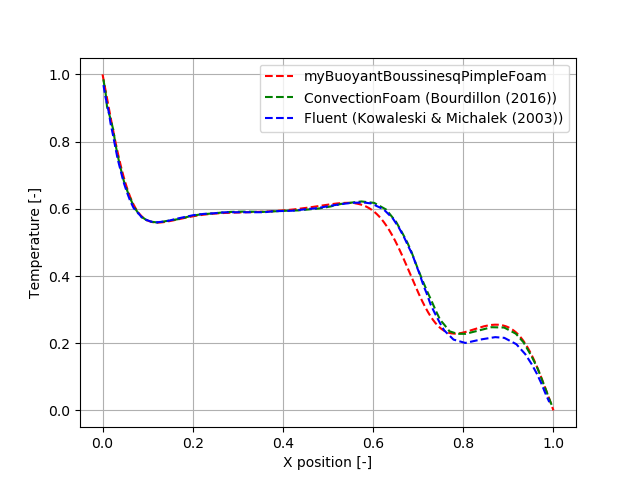
\includegraphics[width=\linewidth]{temperature_xpos_conv.png}\hfill
		\caption{Temperature along horizontal line.} \label{3.6afig}
	\end{subfigure}
	\hfill
	\begin{subfigure}{0.50\textwidth}
		\centering
		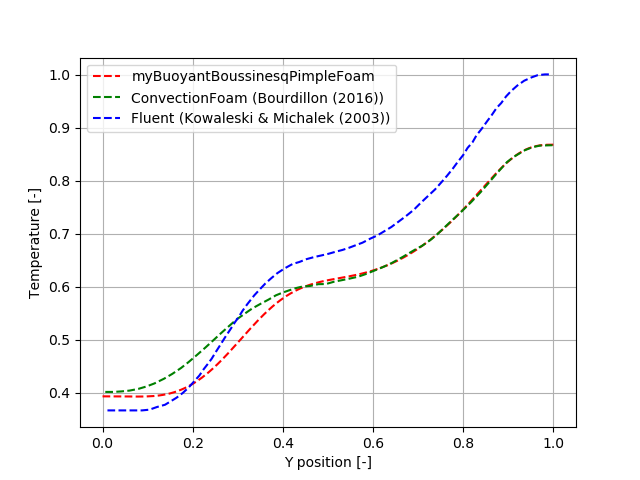
\includegraphics[width=\linewidth]{temperature_ypos_conv.png}	
		\caption{Temperature along vertical line.}\label{3.6bfig}
	\end{subfigure}
	\begin{subfigure}{0.50\textwidth}
		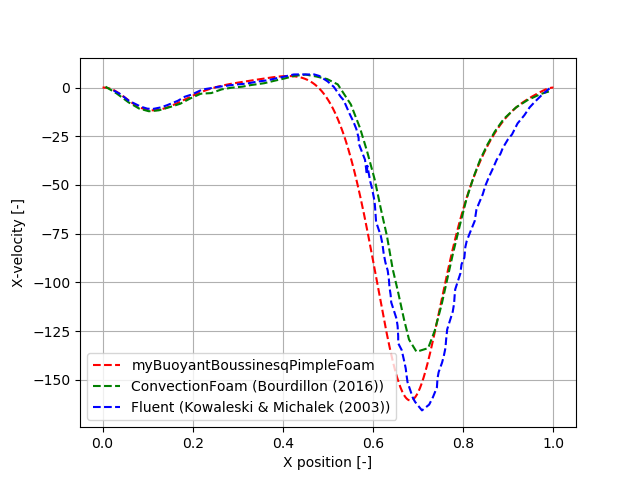
\includegraphics[width=\linewidth]{xvel_xpos_conv.png}\hfill
		\caption{U-velocity along horizontal line.}\label{3.6cfig}
	\end{subfigure}
	\begin{subfigure}{0.50\textwidth}
	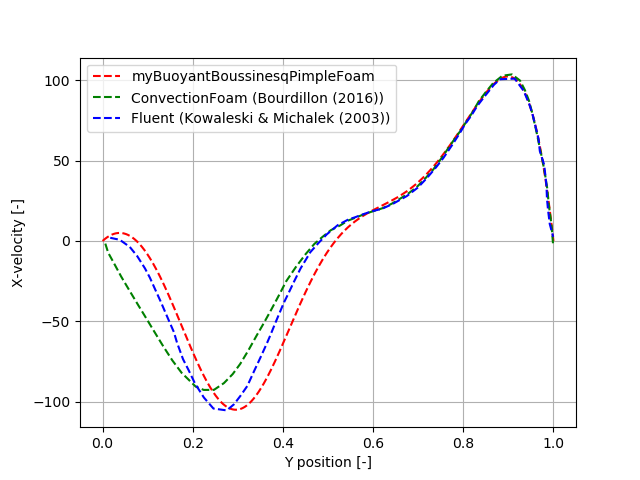
\includegraphics[width=\linewidth]{xvel_ypos_conv.png}	
	\caption{U-velocity along vertical line.}\label{3.6dfig}
	\end{subfigure}
	\begin{subfigure}{0.50\textwidth}
	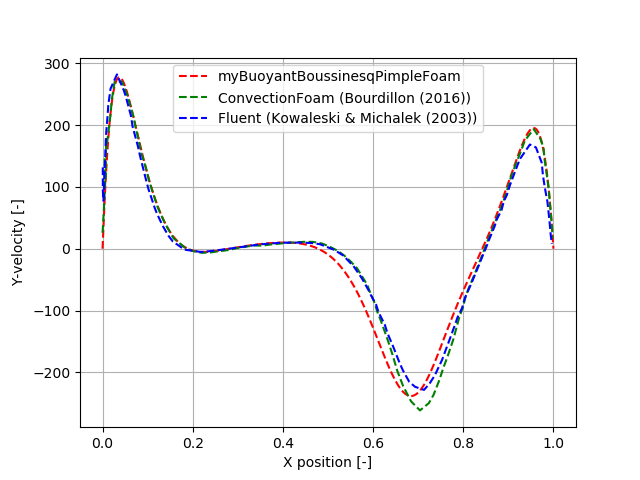
\includegraphics[width=\linewidth]{yvel_xpos_conv.png}\hfill	
	\caption{V-velocity along horizontal line.}\label{3.6efig}
	\end{subfigure}
	\begin{subfigure}{0.50\textwidth}
	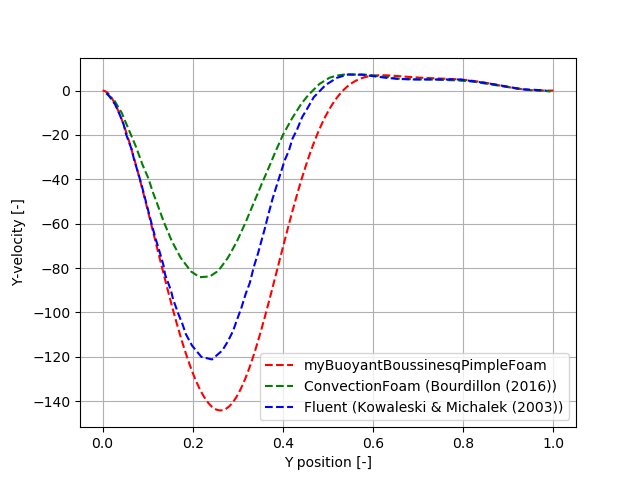
\includegraphics[width=\linewidth]{yvel_ypos_conv.png}	
	\caption{V-velocity along vertical line.}\label{3.6ffig}
	\end{subfigure}
	\caption{Adimensional magnitudes comparison.}
	\label{3.6fig}
\end{figure} 

In the table \ref{3.7tab}, there are shown the temperature, velocity magnitude and density distributions at different time steps. From these images, it can be understood the physical phenomena arising in the natural convection of the problem proposed. At time 100s, the left wall, initiallized at 283K, induces the propagation of the hottest flow through the volume of control and towards the right wall which is initially at 273K. Through time, it is observable how the coldest flow and thereby the less dense, is driven to the bottom region of the cavity while the denser one is redirected over the top. Another remarkable fact is that two flows are originated due to this density inversion point. One emerged near the left wall which moves clockwise and the other one arisen in the mid-bottom part of the right wall which moves on the opposite direction, thus, counter clockwise. This phenomena exhibits by the fact that the density variation is characterized by a polynomial function and it is of importance since this behavior has an impact in the ice layer formation.
\begin{table}[h!]
	\begin{tabular}{@{}lllll@{}}
		\toprule[1pt]
		\multicolumn{1}{c}{\textbf{t = 100s}} & \multicolumn{1}{c}{\textbf{t = 250s}} & \multicolumn{1}{c}{\textbf{t = 1500s}} \\ \midrule[2pt] 
		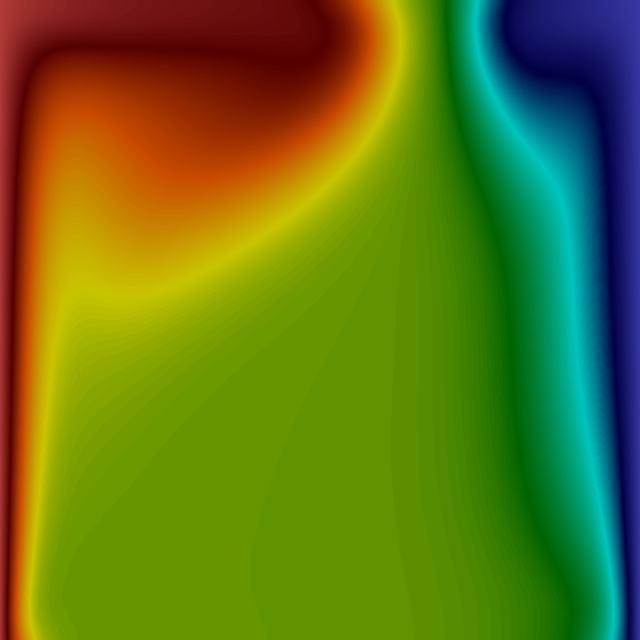
\includegraphics[width=.25\linewidth]{CF_T_100s.png} & 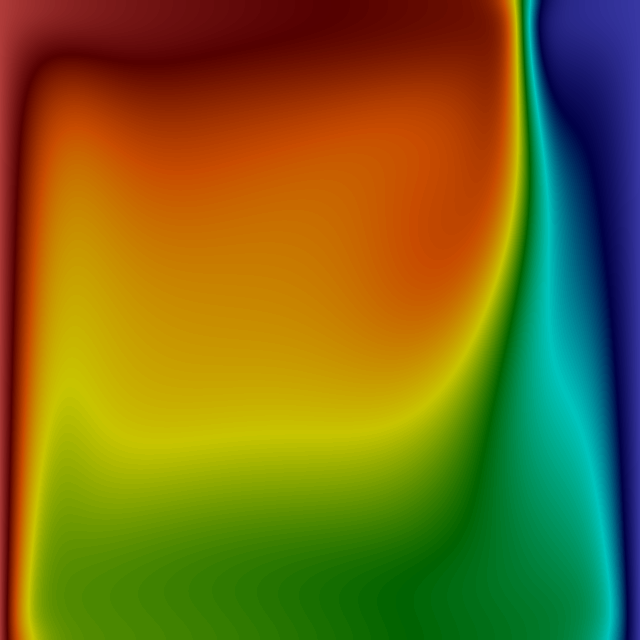
\includegraphics[width=.25\linewidth]{CF_T_250s.png} & 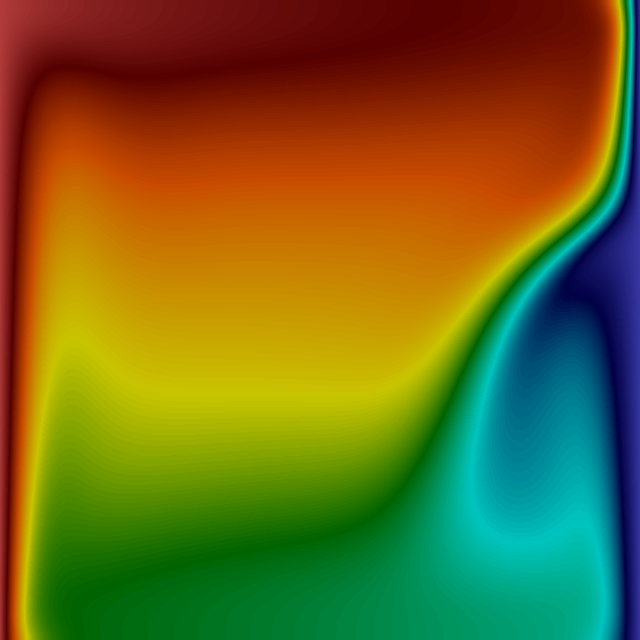
\includegraphics[width=.25\linewidth]{CF_T_1500s.png} & 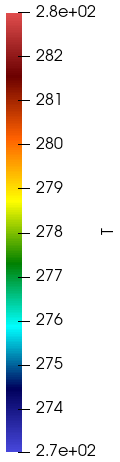
\includegraphics[width=.0658\linewidth]{t.png} \\
		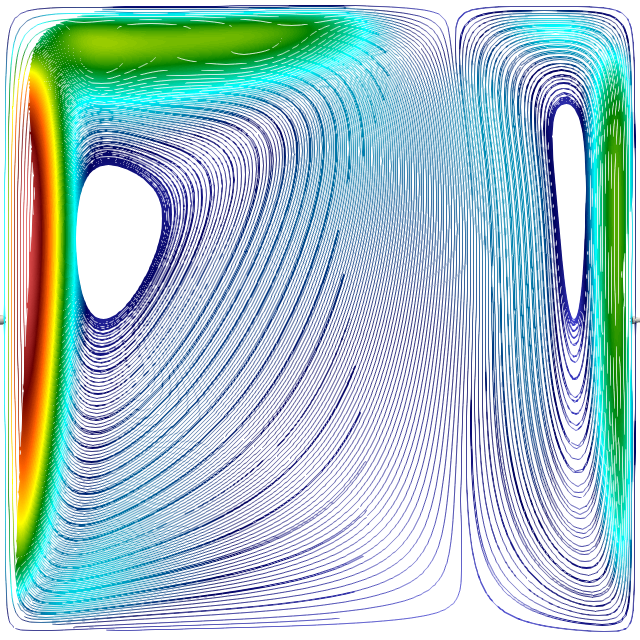
\includegraphics[width=.25\linewidth]{CF_U_100s.png} & 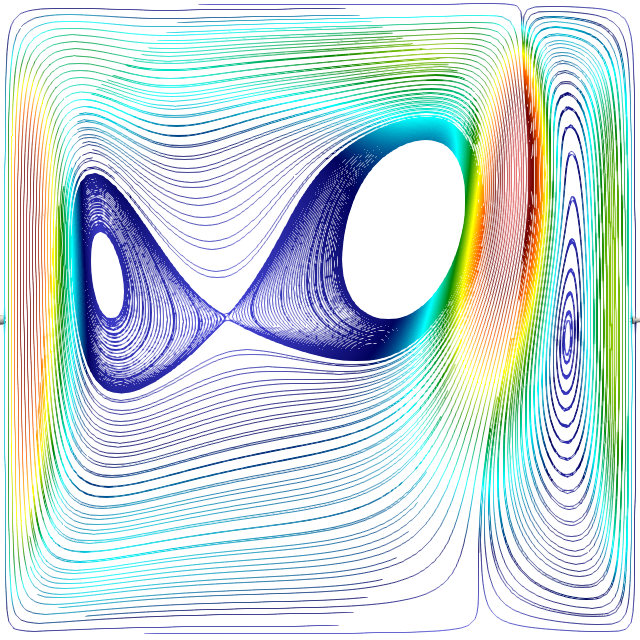
\includegraphics[width=.25\linewidth]{CF_U_250s.png} & 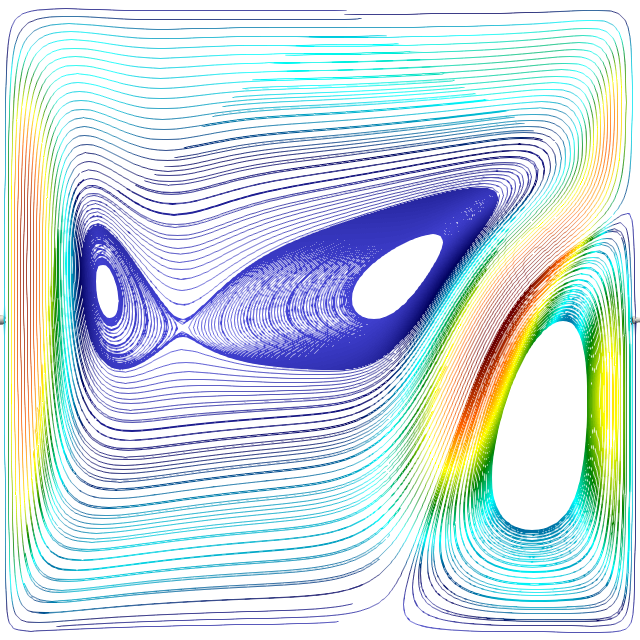
\includegraphics[width=.25\linewidth]{CF_U_1500s.png} & 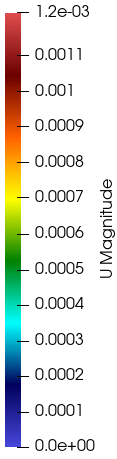
\includegraphics[width=.0658\linewidth]{u.png} \\
		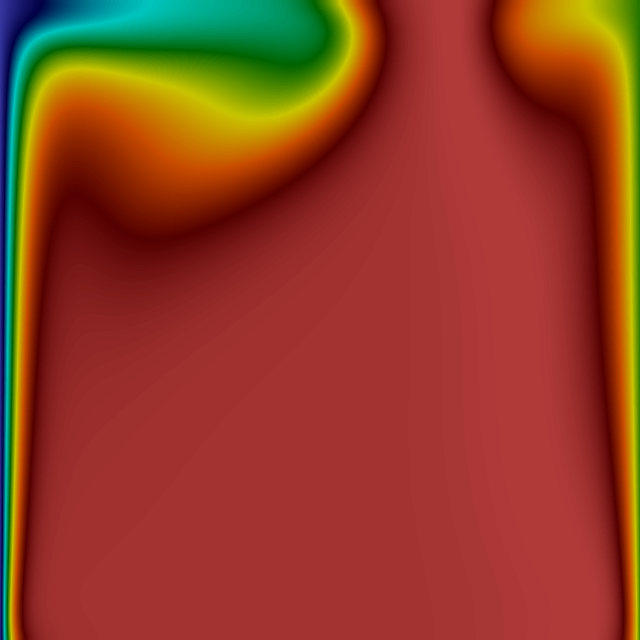
\includegraphics[width=.25\linewidth]{CF_rho_100s.png} & 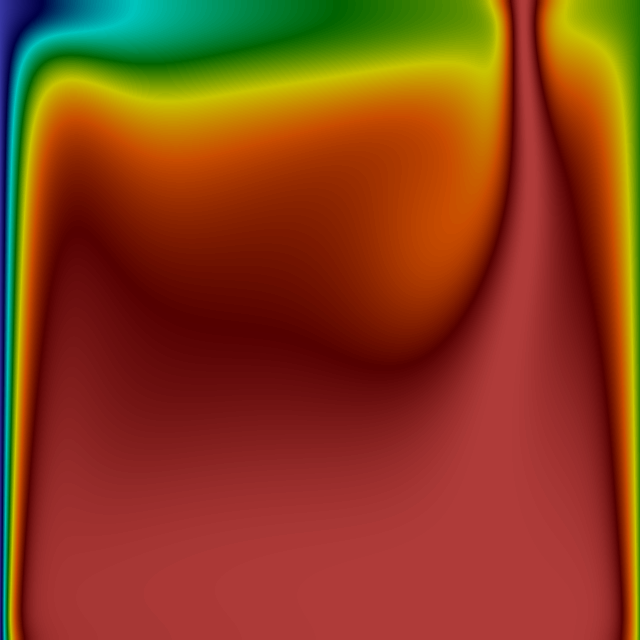
\includegraphics[width=.25\linewidth]{CF_rho_250s.png} & 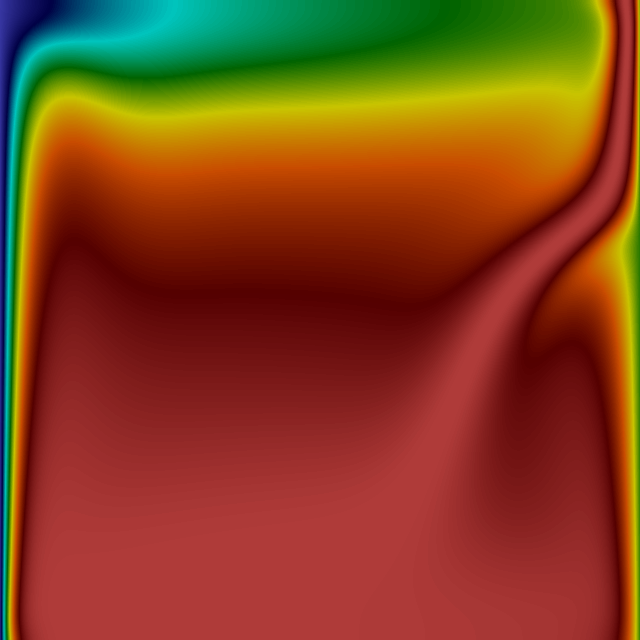
\includegraphics[width=.25\linewidth]{CF_rho_1500s.png} & 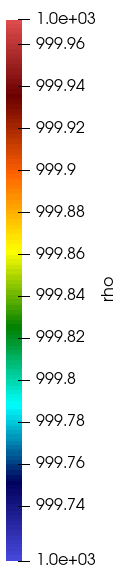
\includegraphics[width=.0558\linewidth]{rho.png} \\ \bottomrule[1pt]		
	\end{tabular}
	\centering
	\caption{Numerical results of natural convection modified solver between \textit{t = 100s} and \textit{1500s}.}	
	\label{3.7tab}
\end{table}
\newline
\noindent In the table shown below are compared the temperature, velocity magnitudes and density distributions for \textit{t = 750s} and \textit{1500s}. As it is observable, between these time steps, the magnitudes do not change substantially and, therefore, one could say that a quasy-steady state is obtained. The solution at \textit{1500s} is used as initial condition for the process of solidification. In the next chapter is commented the concept behind this assumption.
\begin{table}[h!]
	\begin{tabular}{@{}lllll@{}}
		\toprule[1pt]
		\multicolumn{1}{c}{\textbf{t = 750s}} & \multicolumn{1}{c}{\textbf{t = 1500s}} \\ \midrule[2pt] 
		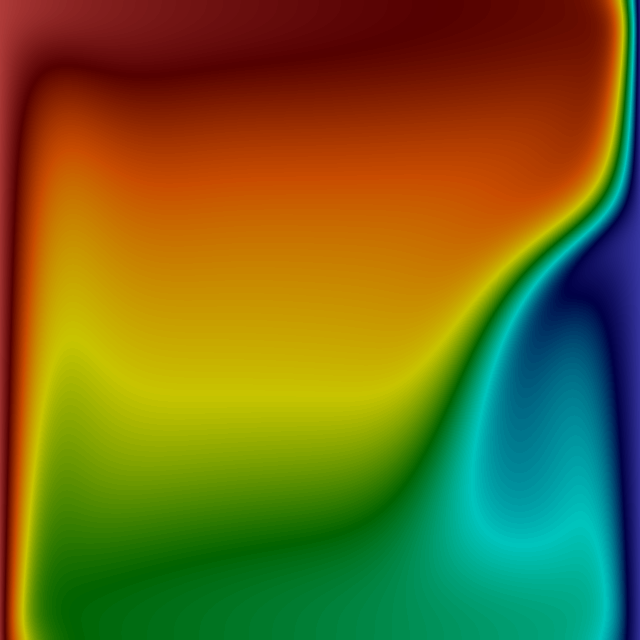
\includegraphics[width=.25\linewidth]{T_750s_CF.png} & 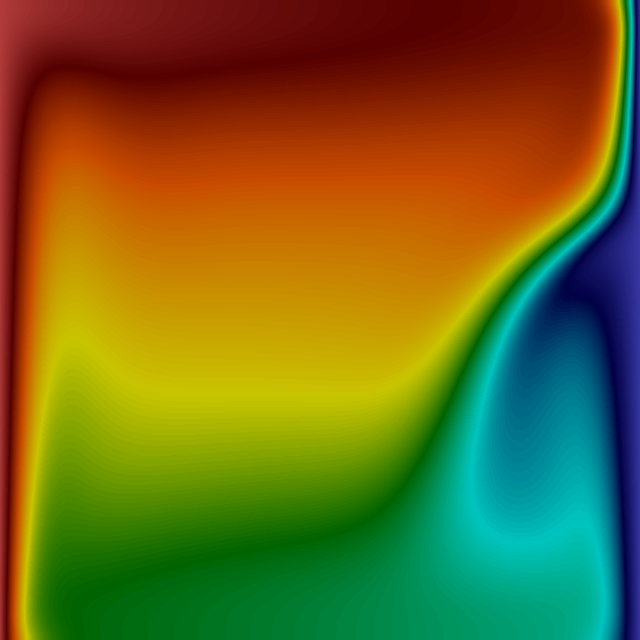
\includegraphics[width=.25\linewidth]{CF_T_1500s.png} & 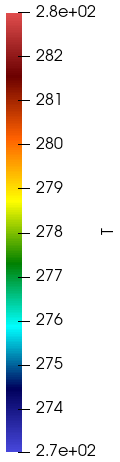
\includegraphics[width=.0658\linewidth]{t.png} \\
		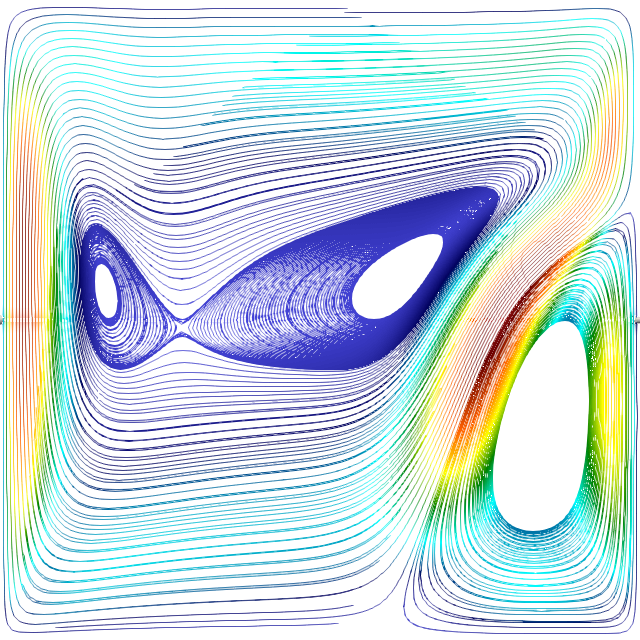
\includegraphics[width=.25\linewidth]{U_750s_CF.png} &  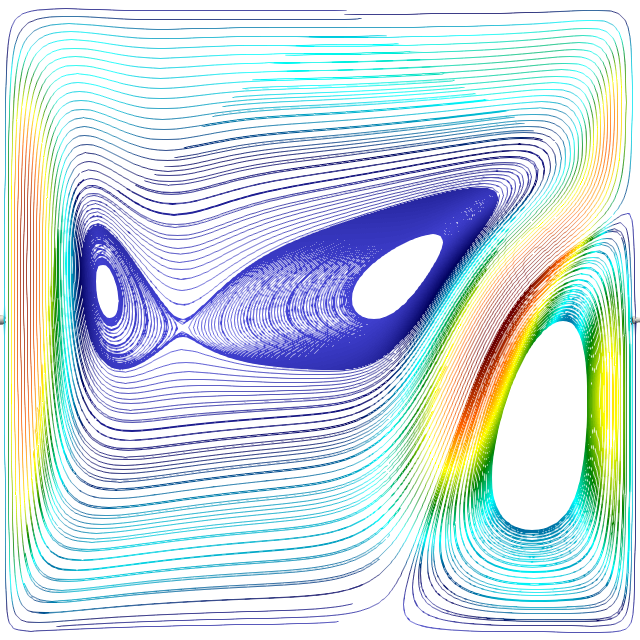
\includegraphics[width=.25\linewidth]{CF_U_1500s.png} & 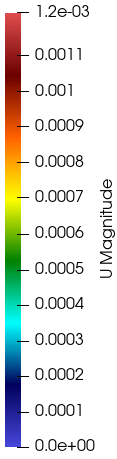
\includegraphics[width=.0658\linewidth]{u.png} \\
		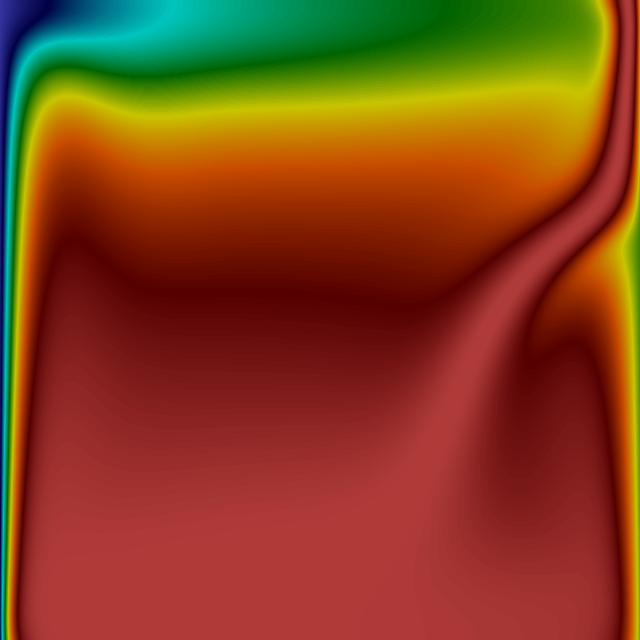
\includegraphics[width=.25\linewidth]{rho_750s_CF.png} &  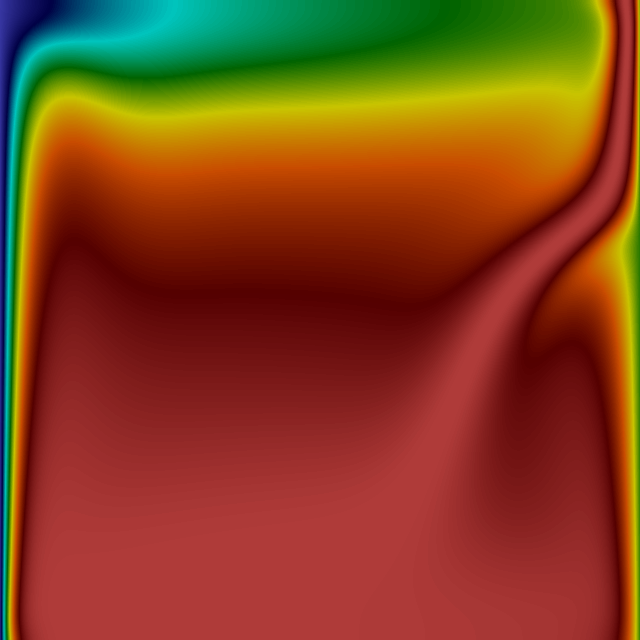
\includegraphics[width=.25\linewidth]{CF_rho_1500s.png} & 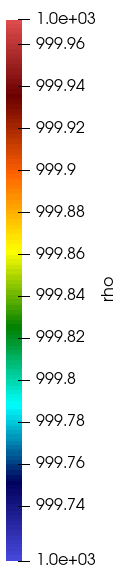
\includegraphics[width=.0558\linewidth]{rho.png} \\ \bottomrule[1pt]		
	\end{tabular}
	\centering
	\caption{Numerical results of Natural convection modified solver between \textit{t = 750s} and \textit{1500s}.}	
	\label{3.7tab}
\end{table}

\clearpage
\section{OpenFOAM: IcoReactingMultiphaseInterFOAM. Phase-Change Process}
\setlength{\parindent}{0.5cm} The solidification process is assessed in this section with two elaborated models. Both of the models are implemented within a multi-phase solver based on the volume of fluid technique. This technique aims to capture interface and enhances contact angle and surface tension for each phase. Thus, the first model is based on the coupling of the VOF and the enthalpy-porosity method. To accomplish the inclusion of the enthalpy-porosity method, a library in which the latent heat is implemented as an explicit source term for the energy equation in the solver. 

\noindent On the other hand, the second model uses the VOF method combined with a semi-empirical model based on the work of Lee. The empirical constant is adapted here to be used in conjunction with the use of the \textit{Classical Nucleation Theory}.

\section{Case Description.}

\setlength{\parindent}{0.5cm} Two regular geomtries are created: a squared cavity, used in the pure convection case and a cylindrical plane geometry. Both geometries test both solidification models.

\begin{figure}[h!]
	\centering
	\begin{subfigure}{\linewidth}
		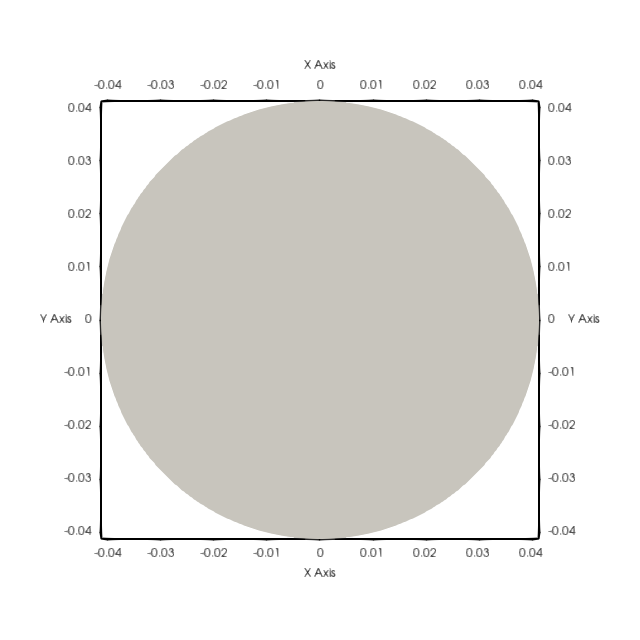
\includegraphics[width=.55\linewidth]{cylinder_geom.png}\hfill
		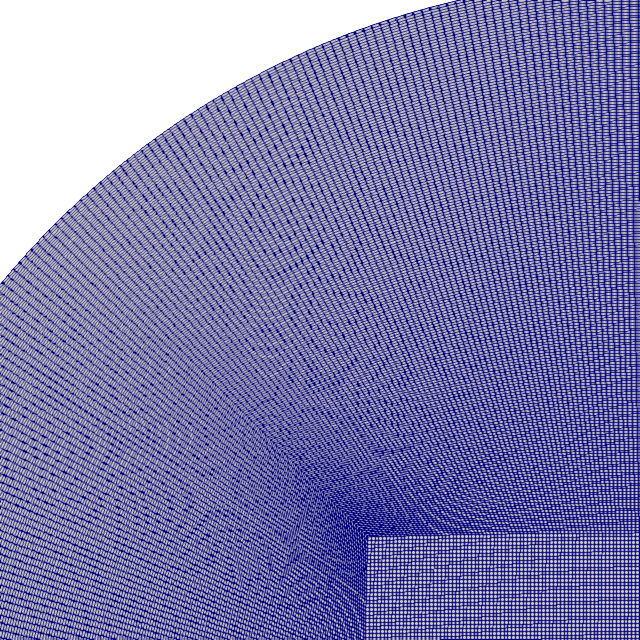
\includegraphics[width=.35\linewidth]{mesh_cylinder.png}	
		\label{BBPF_NCMF}
	\end{subfigure}
	\label{3.7fig}
	\caption{Geometric characteristics for cylinder.}
\end{figure} 
The computed structured mesh consists of 572404 nodes.

\subsection{Hypotheses And Assumptions}

\setlength{\parindent}{0.5cm} To carry out the phase-transition process, some assumptions are taken into account so as to simplify the multiphysics ocurring during such arising phenomena. 

\textbf{Laminar regime:} The Reynolds number, computed from the maximum velocity is not high enough to consider turbulent effects. 

\noindent In the current case-scenario, a Prandtl close to 7. 

\textbf{Newtonian fluid:} The viscosity of the fluid is assumed to be constant.
The thermophysical properties treatment is described below.

\textbf{Quasy-steady state:} Bourdillon \cite{bourdillon_2016} used the hypothesis of quasy-steady solution of the natural convective solver as initial condition in the solidification process. As many researchers as Yan et al. \cite{yan_xu_qiu_gang_2017} suggest, water presents a high latent heat of solidification when the heat released during freezing plays a greater role than the transient process of heat accumulation in the layer of the phase being developed. In other words, when the latent heat of the phase change material is larger than its sensible heat, the latter is having little influence on the temperature distribution of the PCM. In such case, the interface is moving slowly and the temperature distribution, at a given time step, keeps constant. Therefore, for comparison purposes against literature results, the solidification process in a cavity is tested using a quasy-steady solution obtained in the pure convection case.

\subsubsection*{Two phase properties}
\setlength{\parindent}{0.5cm} Within a multiphase framework, a model reflects a jump in properties through the interphase. Thus, a smooth transition between phase properties must be achieved.
\begin{equation}
	\lambda=\lambda_{\ell} \alpha_{\ell}+\lambda_{s} f_{s}
	\label{3.35}
\end{equation}
\begin{equation}
	C_{p}=C_{p_{\ell}} \alpha_{\ell}+C_{p_{s}} f_{s}
	\label{3.36}
\end{equation}
\begin{equation}
	\mu=\mu_{\ell} \alpha_{\ell}+\mu_{s} f_{s}
	\label{3.37}
\end{equation}
In the current case-scenario, $C_{p_{s}}=C_{p_{l}}$.

\noindent In the case of polynomial density variation it is settled in a similar manner. The polynomial is not thought to suit negative temperatures, and when the problem is within this range, the density should take ice's density.
\begin{equation}
	\rho(T)^{\prime}=\rho(T) \alpha_{\ell}+\rho_{s} \alpha_{s}
	\label{3.38}
\end{equation}
where $\alpha_{l}$ and $\alpha_{s}$ are liquid and solid volume fractions, respectively.		
\subsection{Governing Equations}

\setlength{\parindent}{0.5cm} This section is devoted to describe the governing equations that the solidification process requires. Beside the presented conservation equation for the volume of fraction needed for the VOF method, Eq. \ref{VOFEQ},
\begin{equation}
	\frac{\partial \alpha_{\text {phase }}}{\partial t}+\frac{\partial\left(\alpha_{\text {phase }} u_{j}\right)}{\partial x_{j}}=0
	\label{VOFEQ}
\end{equation}
in the next sections, momentum and energy equations are revisited.

\subsubsection{Momentum Equation}

\setlength{\parindent}{0.5cm} The momentum equation has the same terms as per each one of the models. Here it is the equation recalled from previous section:
\begin{equation}
	\label{3.39}
	\begin{aligned}
	&\frac{\partial\left(\rho {u}_{i}\right)}{\partial t}+\frac{\partial\left(\rho {u}_{i} {u}_{j}\right)}{\partial x_{j}} \\
	&\quad=-\alpha_{i} \nabla p+\frac{\partial}{\partial x_{j}}\left(\mu \frac{\partial {u}_{i}}{\partial x_{j}}\right)+F_{\sigma i}+S_{u_{i}}
	\end{aligned}
\end{equation}

\subsubsection{Energy Equation}

\setlength{\parindent}{0.5cm} On the other side, the energy equation slightly differs from one model to the other. As pointed out before, here there are recalled both energy equations.
The energy equation for the Enthalpy-porosity model:
\begin{equation}
\begin{aligned}
\frac{\partial (\rho C_{p} T)}{\partial t}+ \nabla \cdot\left(u_{j}\rho C_{p} T\right)+L\left[\frac{\partial (\rho \alpha_{l}\gamma_{l})}{\partial t}+ \frac{\partial (u_{j}\rho \alpha_{l}\gamma_{l})}{\partial x_{j}}\right]=\nabla \cdot\left(k_{i} \nabla T_{i}\right)
\end{aligned}
\label{3.40}
\end{equation}
The energy equation for the Lee model in conjunction with the nucleation theory:
\begin{equation}
\label{3.41}
\frac{\partial (\rho C_{p} T)}{\partial t}+\nabla \cdot\left(u_{j}\rho C_{p} T\right)=\nabla \cdot\left(k_{i} \nabla T_{i}\right)+S_{H_{i}}
\end{equation}

\subsection{Solver description. Control Loop}

\setlength{\parindent}{0.5cm} IcoReactingMultiphaseInterFoam solver is a multiphase, multicomponent incompressible solver based on volume of fluid method. The solver captures the interfaces and includes contact angle and surface tension effects for each phase. Moreover, this solver supports mass and heat transfer across phases.

\subsection{Mass transfer models}
For each pair of phases, two mass transfer models might be used:
\begin{itemize}
	\item \textbf{Lee model:} Used for solid melting and liquid solidification.
	\item \textbf{KineticGasEvaporation:} Used for condensation and evaporation.
\end{itemize}
In this thesis, only the Lee model will be considered for further explanation.


\subsection{Code implementations}

\setlength{\parindent}{0.5cm} Within the entalphy-porosity model, the source term belonging to the calculation of the latent heat is added within the OpenFOAM framework. The energy equation of the solver shown in Eq. \ref{3.41} is thereby implemented in Fig. \ref{3.8fig}
\begin{figure}[h!]
	\centering
	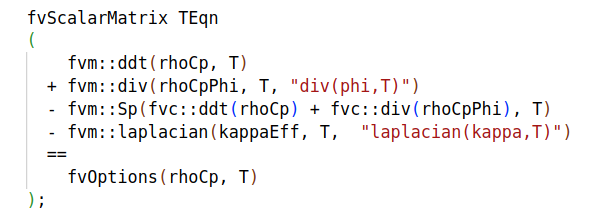
\includegraphics[width=0.6\linewidth]{TEqn.png}\hfill	
	\caption{Energy equation of IcoReactingMultiphaseInterFoam.}
	\label{3.8fig}
\end{figure}
In the term belonging to the RHS of the equation, the solver calls the implemented library \textit{mySolidificationMeltingSource} that calculates the latent heat source term as it appears in the figure \ref{3.9fig}:
\begin{figure}[h!]
	\centering
	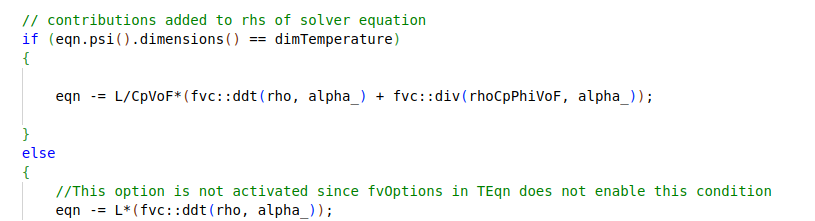
\includegraphics[width=0.8\linewidth]{solidification_latent_heat.png}\hfill
	\caption{Latent heat source term present in mySolidificationMeltingSource library.}
	\label{3.9fig}
\end{figure}

\noindent Here, the alpha variable showing up in the calculation is obtained through a linear expression that gives the amount of energy contained in the fluid cell above the melting point. This is divided by the latent heat to obtain the liquid fraction. Then, this fraction is constained between 0 and 1. Further details on the code can be found in \ref{Enthalpy-porosity library}. The liquid fraction is calculated instead of being obtained through the transport equation worked out within the VOF method so it can be used in other solvers. This is explained later in this thesis.

The \textbf{rhoCpPhiVoF} term, which is called in this library, is created in \textit{createFields.H} as a variable field so that it can be called from everywhere within the code.
\clearpage
\begin{figure}[h!]
	\centering
	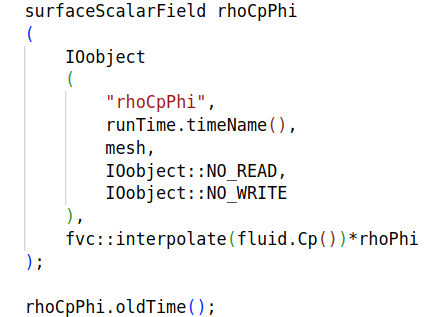
\includegraphics[width=0.4\linewidth]{rhocpphicreate.png}\hfill	
	\caption{\textbf{rhoCpPhi} field in \textit{createFields.H}}
	\label{3.10fig}
\end{figure}
 
\noindent The implemented library can be found in the Appendix \ref{AppendixA}, section \ref{Enthalpy-porosity library}. 

\noindent On the core of the other model, the basis of the Lee model is already implemented in OpenFOAM. However, there is a parameter, \textit{C}, devoted to act as a condensation rate. This is referred as an empirical coefficient used to speed-up or slow down the mass and heat transfer. The physics behind are unknown for this solver, therefore, in favor of tunning this parameter in accordance with the characteristic behavior of the water when it freezes, the \textit{Classical Nucleation theory} is followed.
\newline
\begin{figure}[h!]
	\centering
	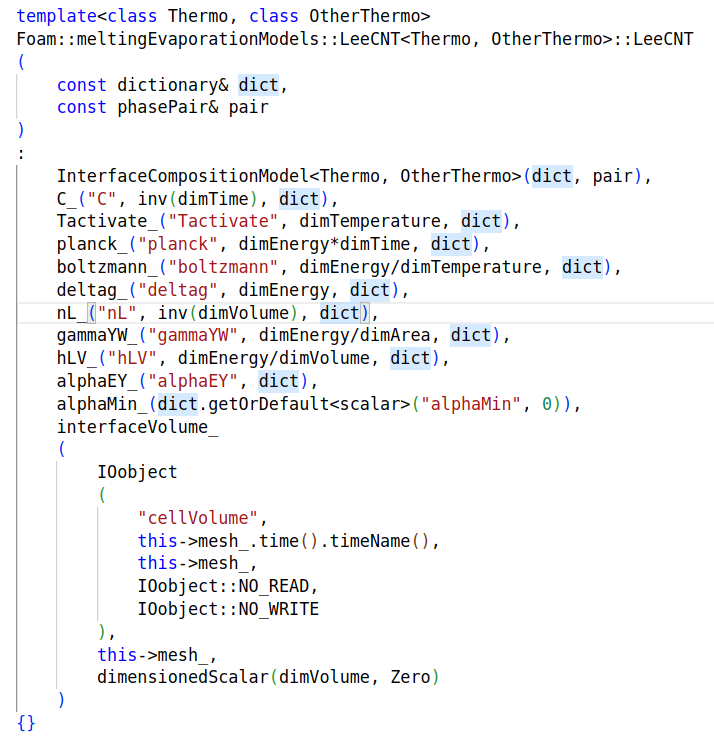
\includegraphics[width=0.6\linewidth]{LeeCNT.png}\hfill	
	\caption{Library function in LeeCNT.}
	\label{3.11fig}
\end{figure}
\newline
In the function shown above, all of the parameters concerning the formulas required to calculate the nucleation rate of the water are user-defined parameters except for the \textbf{cellVolume} which is an implicit function that calculates the volume per each cell. In the Appendix \ref{AppendixA}, the code related with the Lee model using this theory can be found.

\subsection{Case Setup}
\subsubsection*{Boundary conditions}

For the squared cavity:
The initial conditions for the internal field of the cavity regarding the velocity, temperature and pressure magnitudes are inherited from the last timestep of the natural convection case under the assumption of quasi-steady state. The temperature of the right wall is suddenly decreased to 263K.

\begin{table}[h!]
	\begin{tabular}{@{}lllll@{}}
		\toprule[1pt]
		\textbf{Boundary} & \textbf{Conditions}  \\ \midrule[2pt]
		Left & $T_{l}=283, v_{l} = 0, \frac{\partial \alpha_{l}}{\partial n} = 0, \frac{\partial \alpha_{s}}{\partial n} = 0    $  \\
		Right & $T_{r}=263, v_{r} = 0, \alpha_{l} = 1, \alpha_{s} = 0 $ \\
		Upper & $\frac{\partial T_{u}}{\partial n} = 0, v_{u} = 0, \frac{\partial \alpha_{l}}{\partial n} = 0, \frac{\partial \alpha_{s}}{\partial n} = 0$  \\
		Bottom & $\frac{\partial T_{b}}{\partial n} = 0, v_{b} = 0, \frac{\partial \alpha_{l}}{\partial n} = 0, \frac{\partial \alpha_{s}}{\partial n} = 0 $  \\ \bottomrule[1pt]		
	\end{tabular}
	\centering
	\caption{Boundary conditions for natural convection case. Cavity case.}	
	\label{3.8tab}
\end{table}

\noindent frontAndBack boundary is set to \textit{empty} to define a 2-dimensional case-scenario. 

For the cylinder:
\begin{table}[h!]
	\begin{tabular}{@{}lllll@{}}
		\toprule[1pt]
		\textbf{Boundary} & \textbf{Conditions}  \\ \midrule[2pt]
		Walls & $T=255, v = 0,\frac{\partial \alpha_{l}}{\partial n} = 0, \frac{\partial \alpha_{s}}{\partial n} = 0    $  \\
		Internal field & $T=294, v = 0, \alpha_{l} = 1, \alpha_{s} = 0 $ \\
		\bottomrule[1pt]		
	\end{tabular}
	\centering
	\caption{Boundary conditions for natural convection case. Cylinder case.}	
	\label{3.9tab}
\end{table}

\noindent As in the previous geometry, there is an empty boundary called frontAndBack to define a planar case.

\noindent The thermophysical properties and solver parameters defined below are setted up for both geometries.
\clearpage
\subsubsection*{Thermophysical properties}
\begin{table}[h!]
	\begin{tabular}{@{}lllll@{}}
		\toprule[1pt]
		\textbf{Water properties} & \textbf{Symbol} & \textbf{Values} & \textbf{Units} &  \\ \midrule[2pt]
		Water density & $\rho_l$ & 999.8 & $kg.m^{-3}$ \\
		Ice density & $\rho_s$ & 916.8 & $kg.m^{-3}$ \\		
		Water kinematic viscosity & $\nu_{l}$ & 1.79e-6 & $m^{2}.s^{-1}$ \\
		Ice kinematic viscosity & $\nu_{s}$ & 2.0e-6 & $m^{2}.s^{-1}$ \\		
		Water thermal conductivity & $\lambda_{l}$ & 0.56 & $W.m^{-1}.K^{-1}$ \\
		Ice thermal conductivity & $\lambda_{s}$ & 2.26 & $W.m^{-1}.K^{-1}$ \\		
		Heat capacity & $C_{p_{l}}=C_{p_{s}}$ & 4202 & $J.kg.K^{-1}$ \\		 
		Gravitational acceleration & $g$ &  9.81  & $m.s^{-2}$ \\
		Thermal diffusivity & $\gamma$ &  1.435e-7  & $m^{2}.s^{-1}$ \\		
		Thermal expansion coefficient & $\beta$ &  6.734e-5  & $K^{-1}$ \\
		Latent heat & $L$ &  335000  & $J.K^{-1}$ \\			
		Laminar Prandtl number & $P_r$ &  6.99  & - \\
		Reference temperature & $T_r$ &  6.734e-5  & $K$ \\
		Darcy's constant & $D_c$ &  10e8  & - \\		 \bottomrule[1pt]		
	\end{tabular}
	\centering
	\caption{Water properties for natural convection.}	
	\label{3.10tab}
\end{table}
In table \ref{3.11tab} are detailed the parameters used in the implemented nucleation library for the Lee model.
\begin{table}[h!]
	\begin{tabular}{@{}lllll@{}}
		\toprule[1pt]
		\textbf{Water nucleation properties} & \textbf{Symbol} & \textbf{Values} & \textbf{Units} &  \\ \midrule[2pt]
		Planck constant & $h$ & 6.63e-34 & $J.s$ \\
		Boltzmann constant & $k_{B}$ & 1.38e-23 & $J.K^{-1}$ \\		
		Gibbs free energy & $\Delta_{gv}$ & 4e-20 & $J$ \\
		Interfacial tension & $\gamma_{yw}$ & 2.91e-2 & $J.m^{-2}$ \\		
		Latent heat per volume & $H_{lv}$ & 3.10e8 & $J.m^{-3}$ \\
		Shape coefficient of nucleation & $\alpha_{ey}$ & 0.0001 & - \\		
		Water molecule per volume & $n_{L}$ &  5.5e4  & $m^{3}$ \\		 \bottomrule[1pt]		
	\end{tabular}
	\centering
	\caption{Water properties for solidification.}	
	\label{3.11tab}
\end{table}
The solver parameters used for the discretization of the different terms in the equations are pointed out next. 

\subsubsection*{Solver parameters}
So as to obtain a minimum expected accuracy during the calculation, in table \ref{3.13tab} are the chosen parameters for the equation solvers.
\clearpage
\begin{table}[h!]
\begin{adjustbox}{width=1\textwidth}
	\small		
	\begin{tabular}{@{}lllll@{}}
		\toprule[1pt]
		\textbf{Equation} & \textbf{Linear Solver} & \textbf{Smoother/Preconditioner} & \textbf{Tolerance} &  \\ \midrule[2pt]
		Pressure correction equation (P) & PCG & DIC & 1e-5 \\
		Momentum equation (U)& smoothSolver & symGaussSeidel  & 1e-06 \\
		Volume fraction equation (alpha) & smoothSolver & symGaussSeidel  & 1e-8 \\
		Species equation  (Y)   & smoothSolver   & symGaussSeidel &1e-09 \\		 
		Energy equation (T)    &  PBiCG  &  DILU
		&  1e-08  \\ \bottomrule[1pt]		
	\end{tabular}
\end{adjustbox}
	\centering
	\caption{Solvers for the discretised equations.}	
	\label{3.13tab}
\end{table}
\clearpage
\subsection{Validation of Results and Conclusions}
\label{Convection-case}
\setlength{\parindent}{0.5cm} The validation of the phase change problem is achieved by different methodologies. First, the enthalpy-porosity and Lee-CNT models are compared with available data found in the doctoral thesis of Borudillon \cite{bourdillon_2016} and the experimental data of Kowalewski et al. \cite{kowalewski_rebow_1999}. And later, the Lee-CNT model is tested against the classical Stefan problem.

\noindent So as to understand the physical phenomena underlaying these plots, a first general explanation is given. 

\noindent In figure \ref{3.13figa}, temperature distribution along x mid-plane shows a first sudden decrease whithin the initial position and $x < 0.2$ due to the existing temperature gradient between the left wall and the internal field temperature obtained from the quasi-steady solution in the natural convection solver. After that, nearly $0.1 \leq x \leq 0.2$, and induced by the upper clockwise recirculation, the temperature along this mid-plane and until $x \approx 0.6$, is submitted to an increase. From there on, the existence of two colliding and opposite recirculating flows induce a second decrease of the temperature which lasts until $x \approx 0.9$. Then, the influence of the proximity with the cold wall makes the temperature dimensionless to undergo a fast decrease.

\noindent If one recalls now in the temperature distribution along the vertical mid-plane, Fig. \ref{3.13figb}, it is depicted how the temperature increases slowly at the bottom of the cavity $0 \leq y \leq 0.2$. This is mainly due to the gravity related terms which determine the buoyancy effects within the domain. Thereafter, when in the range of $0.2 \leq y \leq 0.4$ there is an increase speed-up by the effects of the recirculating flows colliding with each other. From $y \approx 0.4$ towards the top of the cavity, the recirculating flow induces a slowly increase in the temperature.

\noindent Moving along the U-velocity dimensionless component, ,Fig. \ref{3.13figc}, a first oscillation is observed near the left wall at $x \approx 0.1$. Then, at $0.6 \leq x \leq 0.8$, it shows up a sudden decrease in the velocity magnitude due the clockwise direction that the upper flow exhibits as long as the ice layer formation advances in time. From $0.7 \leq x \leq 1$ the velocity component increases rapidly until it reaches a 0 constant value due to the appearence of the solid ice layer. 

\noindent Describing the U-velocity profile along the vertical line, Fig. \ref{3.13figd}, one sees how the first negative peak in $0.2 \leq y \leq 0.3$ is highly influenced by the effect of the counter clockwise lower recirculating flow generated by the upper flow (rotating clockwise) when interacts with the ice layer advancing front. Moving up along the vertical line, the behavior of the velocity component tends to increase since it starts being influenced by the upper recirculating flow, in $0.3 \leq y  \leq 0.9$, and until it reaches a 0 value induced by the adiabatic and the zero gradient velocity condition applied in top and bottom walls.

\noindent Similarly, the V-velocity along the x mid-plane, Fig. \ref{3.13figc}, displays a peak near the left wall where the direction of the upper flow is clockwise. As one moves farther from the left wall, the velocity components are not constituted yet. Comparatively as with the U-velocity along the x mid-plane, the influence of the lower recirculating flow brings negative dimensionless velocity vectors in the vertical magnitudes. This is in the region where $0.6 \leq x \leq 0.7$. At $0.75 \leq x \leq 0.8$ the recirculating flows in this region slightly influences the increase of the velocity. From there on, the velocity gets reduced until it reaches a zero constant value due to the sink of velocity magnitude in the ice layer zone.

\noindent Finally, the V-velocity plotted along the y mid-plane depicts a negative peak at $y \approx 0.3$. This is mainly influenced by the negative dimensionless velocity values arising from the recirculating flow taking place from the collision of the upper flow and the ice layer.

\begin{table}[h!]
	\begin{tabular}{@{}b{2cm}ccc@{}}
		\toprule[1pt]
		& 
		\multicolumn{1}{c}{\textbf{Lee model-CNT}} & \\ \midrule[2pt]
		\vbox to 3\baselineskip{\textbf{Temperature}}& 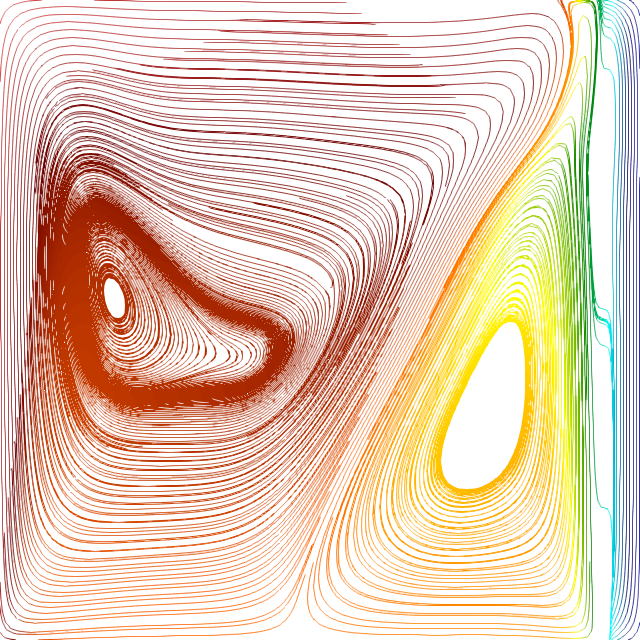
\includegraphics[width=.25\linewidth]{t_x_streamlines.png} & 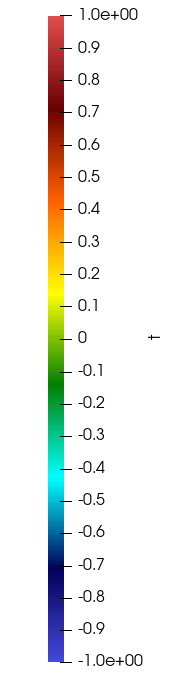
\includegraphics[width=0.078\linewidth]{t_x_scale.png} \\		
		\vbox to 3\baselineskip{\textbf{U-velocity}}&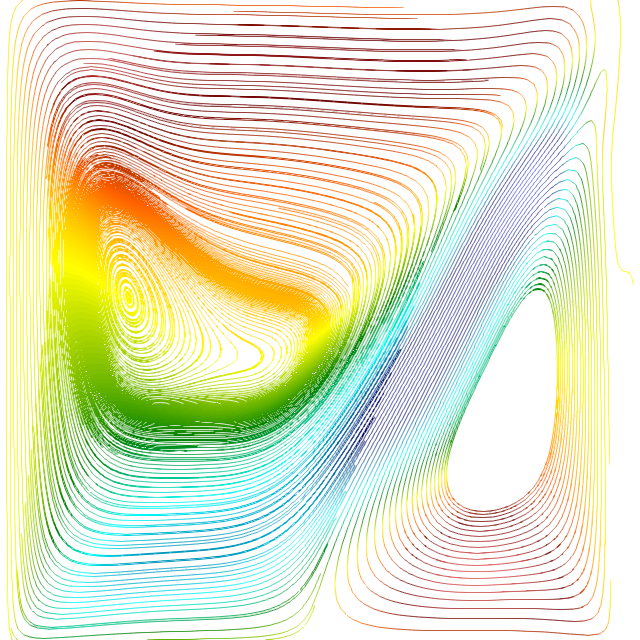
\includegraphics[width=.25\linewidth]{u_x_streamlines.png} & 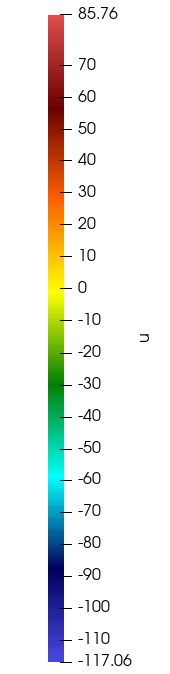
\includegraphics[width=0.078\linewidth]{u_x_scale.png}\\
		\vbox to 3\baselineskip{\textbf{V-velocity}}& \includegraphics[width=.25\linewidth]{v_x_streamlines.png} & \includegraphics[width=0.078\linewidth]{v_x_scale.png} \\	 \bottomrule[1pt]		
	\end{tabular}
	\centering
	\caption{Numerical results of dimensionless magnitudes for Lee-CNT model at \textit{t = 100s}.}	
	\label{3.15tab}
\end{table}


\begin{figure}[h!]
	\begin{subfigure}{0.50\textwidth}
		\centering
		\includegraphics[width=\linewidth]{T_xpos_cavity_comparative.png}\hfill
		\caption{Temperature along horizontal line.} \label{3.13figa}
	\end{subfigure}
	\hfill
	\begin{subfigure}{0.50\textwidth}
		\centering
		\includegraphics[width=\linewidth]{T_ypos_cavity_comparative.png}	
		\caption{Temperature along vertical line.}\label{3.13figb}
	\end{subfigure}
	\begin{subfigure}{0.50\textwidth}
		\includegraphics[width=\linewidth]{xvel_xpos_cavity_comparative.png}\hfill
		\caption{U-velocity along horizontal line.}\label{3.13figc}
	\end{subfigure}
	\begin{subfigure}{0.50\textwidth}
		\includegraphics[width=\linewidth]{xvel_ypos_cavity_comparative.png}	
		\caption{U-velocity along vertical line.}\label{3.13figd}
	\end{subfigure}
	\begin{subfigure}{0.50\textwidth}
		\includegraphics[width=\linewidth]{yvel_xpos_cavity_comparative.png}\hfill	
		\caption{V-velocity along horizontal line.}\label{3.13fige}
	\end{subfigure}
	\begin{subfigure}{0.50\textwidth}
		\includegraphics[width=\linewidth]{yvel_ypos_cavity_comparative.png}	
		\caption{V-velocity along vertical line.}\label{3.13figf}
	\end{subfigure}
	\caption{Adimensional magnitudes comparison at \textit{t = 100s}.}
	\label{3.13fig}
\end{figure}
\clearpage
\noindent Dimensionless quantities presented in the section \ref{Convection-case} are here discussed for solidification comparison purposes. Temperature dimensionless results for the Enthalpy-porosity and Lee-CNT models are in a good agreement with Fluent and IcingFoam results. However, large discrepancies arise in the evolution of the velocity magnitudes. With special mention to U-velocity along x mid-plane, \ref{3.13figc} and V-velocity along y mid-plane, \ref{3.13figf}. Comparatively, the Enthalpy-porosity model tends to overpredict the velocity magnitude with respect to the Lee-CNT model and therefore it predicts a faster formation of a well-developed shape front. The results also show a minimal shift between numerical solutions due to the advancing front which tends to slightly infer in the evolution of the physical magnitudes.

\begin{table}[h!]
	\begin{tabular}{@{}b{2cm}ccc@{}}
		\toprule[1pt]
		 & 
		\multicolumn{1}{c}{\textbf{Enthalpy-porosity}} & \multicolumn{1}{c}{\textbf{Lee model-CNT}} \\ \midrule[2pt]
		\vbox to 3\baselineskip{\textbf{T=100s}}& \includegraphics[width=.25\linewidth]{T_1600s_EP_cavity.png} & \includegraphics[width=.25\linewidth]{T_1600s_CNT_cavity.png} &
		\includegraphics[width=.0658\linewidth]{T_scale_EP_cavity.png} \\		
		\vbox to 3\baselineskip{\textbf{T=200s}}&\includegraphics[width=.25\linewidth]{T_1700s_EP_cavity.png} & \includegraphics[width=.25\linewidth]{T_1700s_CNT_cavity.png} &  \includegraphics[width=.0658\linewidth]{T_scale_EP_cavity.png} \\
		\vbox to 3\baselineskip{\textbf{T=300s}}& \includegraphics[width=.25\linewidth]{T_1800s_EP_cavity.png} & \includegraphics[width=.25\linewidth]{T_1800s_CNT_cavity.png} &
		\includegraphics[width=.0658\linewidth]{T_scale_EP_cavity.png} \\	 \bottomrule[1pt]		
	\end{tabular}
	\centering
	\caption{Numerical results of temperature distributions for Enthalpy-porosity and Lee-CNT models at \textit{t = 100, 200, 300s}.}	
	\label{3.15tab}
\end{table}
\clearpage

\begin{table}[h!]
	\begin{tabular}{@{}b{2cm}ccc@{}}
		\toprule[1pt]
		& 
		\multicolumn{1}{c}{\textbf{Enthalpy-porosity}} & \multicolumn{1}{c}{\textbf{Lee model-CNT}} \\ \midrule[2pt]
		\vbox to 3\baselineskip{\textbf{T=100s}}& \includegraphics[width=.25\linewidth]{U_1600s_EP_cavity.png} & \includegraphics[width=.25\linewidth]{U_1600s_CNT_cavity.png} &
		\includegraphics[width=.0658\linewidth]{U_scale_1600s_cavity.png} \\		
		\vbox to 3\baselineskip{\textbf{T=200s}}&\includegraphics[width=.25\linewidth]{U_1700s_EP_cavity.png} & \includegraphics[width=.25\linewidth]{U_1700s_CNT_cavity.png} &  \includegraphics[width=.0658\linewidth]{U_scale_1700s_cavity.png} \\
		\vbox to 3\baselineskip{\textbf{T=300s}}& \includegraphics[width=.25\linewidth]{U_1800s_EP_cavity.png} & \includegraphics[width=.25\linewidth]{U_1800s_CNT_cavity.png} &
		\includegraphics[width=.0658\linewidth]{U_scale_1800s_cavity.png} \\	 \bottomrule[1pt]		
	\end{tabular}
	\centering
	\caption{Numerical results of velocity distributions for Enthalpy-porosity and Lee-CNT models at \textit{t = 100, 200, 300s}.}	
	\label{3.16tab}
\end{table}
\noindent In the figures shown in the tables \ref{3.15tab}, \ref{3.16tab}, and \ref{3.17tab} are depicted the main physical phenomena of the solidification process. Temperature fields, velocity magnitudes and liquid volume fraction are chosen in order to visually detect the minimum local differences as the phase change gets more developed. As commented above, and shown in table \ref{3.16tab}, the Enthalpy-porosity model overpredicts the velocity magnitude until the extent of exhibiting a well-developed "belly" shape front. Contrarily, the evolution of the velocity magnitude in the Lee-model is under-predicted in comparison with the Enthalpy-porosity model, fact that leads to a more planar shape of the advancing ice layer.
\clearpage
\begin{table}[h!]
	\begin{tabular}{@{}b{2cm}ccc@{}}
		\toprule[1pt]
		& 
		\multicolumn{1}{c}{\textbf{Enthalpy-porosity}} & \multicolumn{1}{c}{\textbf{Lee model-CNT}} \\ \midrule[2pt]
		\vbox to 3\baselineskip{\textbf{T=100s}}& \includegraphics[width=.25\linewidth]{alpha_1600s_EP_cavity.png} & \includegraphics[width=.25\linewidth]{alpha_1600s_CNT_cavity.png} &
		\includegraphics[width=.0658\linewidth]{alpha_scale_cavity.png} \\		
		\vbox to 3\baselineskip{\textbf{T=200s}}&\includegraphics[width=.25\linewidth]{alpha_1700s_EP_cavity.png} & \includegraphics[width=.25\linewidth]{alpha_1700s_CNT_cavity.png} &  \includegraphics[width=.0658\linewidth]{alpha_scale_cavity.png} \\
		\vbox to 3\baselineskip{\textbf{T=300s}}& \includegraphics[width=.25\linewidth]{alpha_1800s_EP_cavity.png} & \includegraphics[width=.25\linewidth]{alpha_1800s_CNT_cavity.png} &
		\includegraphics[width=.0658\linewidth]{alpha_scale_cavity.png} \\	 \bottomrule[1pt]		
	\end{tabular}
	\centering
	\caption{Numerical results of fluid fraction distributions for Enthalpy-porosity and Lee-CNT models at \textit{t = 100, 200, 300s}.}	
	\label{3.17tab}
\end{table}
\noindent In the next figures, simulations have been carried out with a cylindrical geometry for a physical time of \textit{5000s}. Initially good agreement between Lee-CNT and Enthalpy-porosity models compared with Fluent and IcingFoam. As results in table \ref{3.18} show, the evolution of temperature, velocity and liquid fraction magnitudes are quite similar, however, one might appreciate slight differences in the velocity magnitudes from \textit{t = 100s} to \textit{300s}. This will be further commented below.
\clearpage
\begin{table}[h!]
	\begin{tabular}{@{}b{2cm}lll@{}}
		\toprule[1pt]
		&\multicolumn{1}{c}{\textbf{Enthalpy-porosity}} & 
 		\multicolumn{1}{c}{\textbf{Lee model-CNT}} \\ \midrule[2pt]
		\vbox to 3\baselineskip{\textbf{T=100s}}&\includegraphics[width=.25\linewidth]{T_100s_EP.png} & \includegraphics[width=.25\linewidth]{T_100s_CNT.png} &
		\includegraphics[width=.0658\linewidth]{T_scale_100s_EP.png} \\
		\vbox to 3\baselineskip{\textbf{T=300s}}&\includegraphics[width=.25\linewidth]{T_300s_EP.png} &
		\includegraphics[width=.25\linewidth]{T_300s_CNT.png} & 
		\includegraphics[width=.0658\linewidth]{T_scale_300s_EP.png} \\
		\vbox to 3\baselineskip{\textbf{T=100s}}& \includegraphics[width=.25\linewidth]{U_100s_EP.png} & \includegraphics[width=.25\linewidth]{U_100s_CNT.png} &  \includegraphics[width=.0558\linewidth]{U_scale_100s_EP.png} \\
		\vbox to 3\baselineskip{\textbf{T=300s}}& \includegraphics[width=.25\linewidth]{U_300s_EP.png} & \includegraphics[width=.25\linewidth]{U_300s_CNT.png} &  \includegraphics[width=.0558\linewidth]{U_scale_300s_EP.png} \\
		\vbox to 3\baselineskip{\textbf{T=100s}}&\includegraphics[width=.25\linewidth]{alpha_100s_EP.png} & \includegraphics[width=.25\linewidth]{alpha_100s_CNT.png} &  \includegraphics[width=.0558\linewidth]{alpha_scale_cavity.png} \\
		\vbox to 3\baselineskip{\textbf{T=300s}}&\includegraphics[width=.25\linewidth]{alpha_300s_EP.png} & \includegraphics[width=.25\linewidth]{alpha_300s_CNT.png} &  \includegraphics[width=.0558\linewidth]{alpha_scale_cavity.png} \\ \bottomrule[1pt]		
	\end{tabular}
	\centering
	\caption{Numerical results of Enthalpy-porosity and Lee-CNT models at \textit{t = 100s} and \textit{300s} in a cylinder.}	
	\label{3.18tab}
\end{table}
\clearpage
Here in Fig. \ref{zoomInterface} it is shown the description of the interface. There it can be checked the mushy region where the liquid fraction is $0 < \alpha_{l} < 1$.
\begin{figure}[h!]
	\centering
	\includegraphics[width=.3\linewidth]{alpha_zoom.png}	
	\caption{Gradient of the interface between liquid and solid phases for Lee-CNT model.}
	\label{zoomInterface}
\end{figure} 

\noindent In the figure \ref{3.12fig}, temperature magnitude is in the center of the cylinder along time. Here, it can be appreciated three different zones: for $0s < t < 400s$, it belongs to the convection heat transfer period, then, for $400s < t < 4000s$ there exists a mushy zone, the water is loosing heat by this time. For $t > 4000s$ solidification begins. As it might be observed in \ref{3.12fig}, but also in the temperature distribution at \textit{t=300s} in table \ref{3.18}, near $300s < t < 600s$ the effect of the density inversion begins to be visible at $T \approx 5 \deg C$. As it happened for the cavity case, the fact of characterizing the density with a polynomial function allows the solver to see a phenomena which appears in the experimental data of Chen et al.  \cite{chen_lee_1998}.

\noindent Large discrepancies arise as the simulation evolves in time in the Enthalpy-model compared with IcingFoam, Lee-CNT model and the experimental data of Chen et al. For this model, solidification takes longer in the center part of the cylinder. Initially, for $0s < t < 300s$, the evolution of the temperature, velocity and liquid fraction seem to match. However, from this point on, convection tends to decrease, and so it does the rest of variables involved. This clearifies that the enthalpy-porosity model developed in conjunction with the VOF technique does not fit the numerical results found in the literature and the fact that does not match with the experimental data may lead to inaccuracies when representing the physical phenomena of solidification in transient simulations. This difference in the numerical solution is due to the use of an unaccurate expression for the volume of fluid implicitly calculated within the library \ref{Enthalpy-porosity library}.

\begin{figure}[t]
	\centering
	\includegraphics[width=.7\linewidth]{T_time_center_cylinder_comparative.png}	
	\caption{Numerical results of temperature profiles in center position of cylindrical geometry.}
	\label{3.12fig}
\end{figure} 

\noindent For the Lee model based on the \textit{Classical Nucleation Theory}, the results are compared in the next section against the analytical solution given by the Neumann solutions of the Stefan problem.

\clearpage
\subsubsection{Stefan Problem}

\setlength{\parindent}{0.5cm} The Stefan problem, is an initial boundary value problem of a parabolic differential equation with discontinuous coefficients on the phase transitions interfaces. The analytical solution to the classical Stefan problem exists in a limited range of idealized situations.

\noindent The governing equations for a general solid-liquid phase change problem are:

\noindent The heat equation for the solid phase,
\begin{equation}
\rho_{s} c_{s} \frac{\partial T_{s}}{\partial t}=\nabla \cdot\left(k_{s} \nabla T_{s}\right) \quad \text { on } \Omega_{s}
\label{3.42}
\end{equation}
for the liquid phase, advective term is also considered:
\begin{equation}
\rho_{l} c_{l}\left(\frac{\partial T_{l}}{\partial t}+\mathbf{u} \cdot \nabla T_{l}\right)=\nabla \cdot\left(k_{l} \nabla T_{l}\right) \quad \text { on } \Omega_{l}
\label{3.43}
\end{equation}
At the interface, the Stefan condition is satisfied and then,
\begin{equation}
\rho_{s} L(t) V_{n}=\left.k_{s} \nabla T\right|_{\Gamma}-\left.k_{l} \nabla T\right|_{\Gamma} \text { on } \Gamma
\label{3.44}
\end{equation}
where $V_{n}$ is the normal velocity at the interface.
\begin{equation}
T=T_{\mathrm{m}} \quad \text { on } \Gamma
\end{equation}
\subsubsection*{One-dimensional problem}

\setlength{\parindent}{0.5cm} In seek of simplification, and recalling the 1D problem as shown in the figure:
\begin{figure}[h!]
	\centering
	\includegraphics[width=.4\linewidth]{stefan.png}	
	\label{Stefanfig}
	\caption{Schematic diagram of Stefan problem.}
\end{figure} 
\newline
the initial conditions are expressed as \cite{zhao_zhao_xu_2018}:
\begin{equation}
	u_{0}(x)=u_{0}, \quad t=0, \quad x \in[0, L],
	\label{3.45}
\end{equation}
while the boundary conditions are the shown below:
\begin{equation}
	u(0, t)=-20^{\circ}C, \quad \frac{\partial u}{\partial x}(L, t)=0, \quad t>0
	\label{3.46}
\end{equation}
\clearpage
\noindent In table \ref{3.19tab}, there are summarized the boundary conditions applied in the cavity geometry of previous cases.
\begin{table}[h!]
	\begin{tabular}{@{}lllll@{}}
		\toprule[1pt]
		\textbf{Boundary} & \textbf{Conditions}  \\ \midrule[2pt]
		Left & $ T_{l} = 253.15, \alpha_{l} = 1, \alpha_{s} = 0    $  \\
		Right & $\frac{\partial T_{r}}{\partial n} = 0,  \frac{\partial \alpha_{l}}{\partial n} = 0, \frac{\partial \alpha_{s}}{\partial n} = 0  $ \\
		Upper & $\frac{\partial T_{t}}{\partial n} = 0, \frac{\partial \alpha_{l}}{\partial n} = 0, \frac{\partial \alpha_{s}}{\partial n} = 0$  \\
		Bottom & $\frac{\partial T_{b}}{\partial n} = 0, \frac{\partial \alpha_{l}}{\partial n} = 0, \frac{\partial \alpha_{s}}{\partial n} = 0 $  \\ \bottomrule[1pt]		
	\end{tabular}
	\centering
	\caption{Boundary conditions for Stefan problem.}	
	\label{3.19tab}
\end{table}
\newline
\noindent The internal field is initiallized at 283.15 K. The used thermophysical properties as well as the solver parameters are similar to the previous solidification cases.
\newline
The discontinuous exact solutions for the Stefan problem are:
\begin{equation}
	\begin{cases}T_{l}(x, t)=\frac{\operatorname{erfc}\left(\frac{x}{2 \sqrt{a_{1} t}}\right)}{\operatorname{erfc}\left(\lambda \sqrt{\frac{a_{\mathrm{s}}}{a_{1}}}\right)}\left(T_{\mathrm{m}}-T_{0}\right)+T_{0}, & x>\xi(t), \\ 
	T_{\mathrm{s}}(x, t)=\frac{\operatorname{erf}\left(\frac{x}{2 \sqrt{a_{\mathrm{s}} t}}\right)}{\operatorname{erf \lambda }}\left(T_{\mathrm{m}}-T_{\mathrm{b}}\right)+T_{\mathrm{b}},& x \leq \xi(t)  .\end{cases}
	\label{3.47}
\end{equation}
By using a phase change interface condition, a solution to the trascendental equation may be found:
\begin{equation}
	\frac{e^{-\lambda^{2}}}{\operatorname{erf}(\lambda)}+\frac{k_{\mathrm{l}}}{k_{\mathrm{s}}} \sqrt{\frac{a_{\mathrm{s}}}{a_{1}}} \frac{T_{\mathrm{m}}-T_{0}}{T_{\mathrm{m}}-T_{\mathrm{b}}} \frac{e^{-\frac{a_{\mathrm{s}}}{a_{1}} \lambda^{2}}}{\operatorname{erfc}\left(\lambda \sqrt{\frac{a_{\mathrm{s}}}{a_{1}}}\right)}=\frac{\lambda L \sqrt{\pi}}{c_{\mathrm{ps}}\left(T_{\mathrm{m}}-T_{\mathrm{b}}\right)}
	\label{3.48}
\end{equation}
where ${\operatorname{erf(x)}}$ is the complementary error function expressed as $1-{\operatorname{erf(x)}}$.
	
\noindent The secant method is used as the iterative scheme to find the root of the given function with $tol<1e-12$. The root of $\lambda$ is 0.2299545377262345.

\noindent In the following figures, the method is tested against the exact solutions of the Stefan problem. 

\begin{figure}[h!]
	\begin{subfigure}{0.50\textwidth}
		\centering
		\includegraphics[width=\linewidth]{Neumann_CNT_9s.png}\hfill
		\caption{Neumann solution vs numerical solution at \textit{t = 9s}.} \label{3.15figa}
	\end{subfigure}
	\hfill
	\begin{subfigure}{0.50\textwidth}
		\centering
		\includegraphics[width=\linewidth]{Neumann_CNT_9s_relative_error.png}	
		\caption{Relative error of the numerical solution at \textit{t = 9s}.}\label{3.15figb}
	\end{subfigure}
	\caption{Numerical solutions of the Lee model-CNT vs Neumann analytical solutions at \textit{t = 9s}.}
	\label{3.15fig}
\end{figure}

\subsubsection{Interface height}

\setlength{\parindent}{0.5cm} The theoretical solution for the evolution of the interface is:
\begin{equation}
	X(t)=2 \lambda \sqrt{a_{\mathrm{s}} t}
	\label{3.49}
\end{equation}
Alongside, a post-process function to calculate the tracking of position of the interface is done. To do so, the values of the liquid fraction per timestep are first obtained. Thus, these values for each time are read to find the position in which alpha is 0.5. The python code is attached in Appendix \ref{AppendixA}, section \ref{Python code for Stefan Problem}.

\begin{table}[h!]
	\begin{tabular}{@{}lllll@{}}
		\toprule[1pt]
		\multicolumn{1}{c}{\textbf{$\alpha_{l}$}}& & \multicolumn{1}{c}{\textbf{$T$}} & \\ \midrule[2pt] 
		\includegraphics[width=.3\linewidth]{alpha_6s_EP.png} & \includegraphics[width=.075\linewidth]{alpha_scale_EP_6s.png} & \includegraphics[width=.3\linewidth]{T_CNT_9s.png} & \includegraphics[width=.075\linewidth]{T_CNT_9s_scale.png}\\ \bottomrule[1pt]		
	\end{tabular}
	\centering
	\caption{Numerical results of temperature and interface evolution for Lee-CNT model at \textit{t = 9s}.}	
	\label{3.20tab}
\end{table}
\begin{figure}[h!]
	\begin{subfigure}{0.50\textwidth}
		\includegraphics[width=\linewidth]{Neumann_CNT_9s_interface.png}\hfill
		\caption{Interface position in time.}\label{3.16figa}
	\end{subfigure}
	\begin{subfigure}{0.50\textwidth}
		\includegraphics[width=\linewidth]{Neumann_CNT_9s_interface_relative_error.png}	
		\caption{Relative error of interface position in time.}\label{3.16figb}
	\end{subfigure}
	\caption{Numerical solutions of the Lee model-CNT vs Neumann analytical solutions for interface position for \textit{t=0-9s}.}
\label{3.16fig}
\end{figure}

\subsubsection{Conclusions on the Stefan problem}
From the figures \ref{3.16figa} and \ref{3.15figa} it is clearly visible that the Neumann solutions of the Stefan problem for the temperature distribution and the interface position do not match the numerical solution obtained with the Lee model undergoing nucleation characteristics. As depicted, the behavior of the analytical solution is faster than the numerical one. 
 
\noindent The explanation resides behind the theory that macroscale models for phase-change generally take the assumptions of constant thermophysical properties, constant latent heat, $L(t) = L_{m}$ and constant melting/solidification temperatures within phases. 

\noindent Alternatively, in this thesis it is proposed a model (Lee model) in which the $L(t)$ is not constant but dependent of the product of the net mass transfer and the difference of enthalpy of fusion between phases as indicated in Eq. \ref{3.50}. It is also remarkable that density is not constant for the fluid phase due to the implementation of the new equation of state in the solver. Thus, it adds more variability to the latent heat calculation.

\noindent Therefore, as the evolution of the latent heat balances the temperature distribution (it is implicit in the energy equation), so it does the development of the interface position.

\begin{equation}
\label{3.50}
L = \frac{d m_{l s}}{d t}\Delta T\Delta H_{f}=C_{f} \rho_{l} \alpha_{l}\left(\frac{T_{s a t}-T_{l}}{T_{s a t}}\right)\left(T_{sat}-T_{l}\right)(H_{l}-H_{s})
\end{equation}

\noindent In the nanoscale, the surface tension in the interface would affect the solution as well. The melting temperature could not be constant anymore since at the interface the condition that $T = T_{m}$ is not achieved. Leaving, at the interface $\Gamma$:
\begin{equation}
s\left(T-T_{\mathrm{m}}\right)=-\sigma\left(\kappa+\alpha V_{\mathrm{n}}\right) \quad \text { on } \Gamma
\label{3.51}
\end{equation}
as pointed out by Zhao et al. \cite{zhao_zhao_xu_2018}. Where $\kappa$ is the interface curvature,  $\alpha$	is a kinetic coefficient, a proportional constant of the velocity of the interface and the kinetic undercooling, $S$, the entropy density difference between phases and $\sigma$ the surface tension. Being, the kinetic undercooling, the state of equilibrium of the liquid submitted to temperatures under melting point without undergoing phase transition. 

\noindent This means that as the undercooling velocity (velocity of nuclei formation) increases, so it does this coefficient. Therefore, the kinetic coefficient jointly with the surface tensions are also the parameters to account for when modeling phase-changes in a nanoscale.
\chapter{Numerical Simulation of Heat Transfer} % Main chapter title

\label{Chapter4}

\section{OpenFOAM: chtMultiphaseInterFOAM. Conjugate Heat Transfer}
\setlength{\parindent}{0.5cm} The last objective of this thesis is to extend the multiphase solver of the previous section so it can account for multiregion purposes. To do so, a new solver derived from the concept of an existing multiregion solver is implemented. 

\noindent The existing solver, \textit{chtMultiRegionFoam} is developed on the basis that the fluid it solves undergoes the compressible Navier-Stokes equations with buoyancy forces and the energy equation per unit mass with gravity terms as follows:
\subsubsection*{Continuity Equation}
The continuity equation reads as:
\begin{equation}
	\frac{\partial \rho}{\partial t}+\nabla \cdot(\rho \boldsymbol{u})=0
	\label{4.1}
\end{equation}
\subsubsection*{Momentum Equation}
The momentum conservation equation yields as:
\begin{equation}
	\begin{aligned}
		&\frac{\partial \rho \boldsymbol{u}}{\partial t}+\nabla \cdot(\rho \boldsymbol{u} \otimes \boldsymbol{u})=\\
		&-\nabla p_{\mathrm{rgh}}+\nabla \cdot\left[\mu\left\{\nabla \otimes \boldsymbol{u}+(\nabla \otimes \boldsymbol{u})^{\mathrm{T}}\right\}\right]
		-\nabla\left(\frac{2}{3} \mu \nabla \cdot \boldsymbol{u}\right)-\boldsymbol{g} \cdot \boldsymbol{x} \nabla \rho
	\end{aligned}
	\centering
	\label{4.2}
\end{equation}
\subsubsection*{Energy Equation}
The energy equation as listed in the native solver is:
\begin{equation}
	\frac{\partial \rho h}{\partial t}+\nabla \cdot(\rho \boldsymbol{u} h)+\nabla \cdot(\rho \boldsymbol{u} K)=\nabla \cdot\left(\frac{\lambda}{c_{p}} \nabla h\right)+\rho \boldsymbol{u} \cdot \boldsymbol{g}
	\label{4.3}
\end{equation}
where \textit{\textbf{u}} is the velocity vector, \textit{h} is the enthalpy, \textit{K = 0.5*\textbf{u $\cdot$ u}} is the kinetic energy per unit mass, \textit{$p_{rgh}=p-\rho\textbf{g}\cdot\textbf{x}$} the modified pressure so that the momentum equation accounts for the buoyancy terms, and the remaining thermophysical properties, $\mu$, $\lambda$, $C_p$ being the kinematic viscosity, the thermal conductivity and the specific heat accordingly. The energy equation does not include radiation, heat generation term and chemical reaction.

\noindent Therefore, the challenge of this part is to couple the multiphase solver (\textit{IcoReactingMultiPhaseInterFoam}) that allows for the solving of a fluid undergoing phase-change with a solid region.  
\subsection{Case description}

\setlength{\parindent}{0.5cm} Within this new case, a mesh for the solid region is required. To do so, a second structured mesh region is implemented within the framework of a provided script which builts cylindrical computational meshes in OpenFOAM format. The script is attached in Appendix \ref{AppendixB}.
\begin{figure}[h!]
	\centering
	\includegraphics[width=0.6\linewidth]{mesh_CHT.png}	
	\label{4.1fig}
	\caption{Computational mesh for the conjugate heat transfer case.}
\end{figure} 
\newline
In the image shown above, a structured mesh of 731734 nodes is generated.
\subsection{Hypotheses And Assumptions}
\textbf{Heat transfer:} Conductive heat transfer is transferred throughout an isotropic material and convective heat transfer is arisen within the fluid region. 

\textbf{Laminar regime:} The Reynolds number, computed from the maximum velocity is not high enough to consider turbulent effects. 

In the current case-scenario, a Prandtl close to 7. The values used for the laminar Prandtl number calculation are: $\mu = 0.001003 Kg.m^{-1}.s^{-1}$, $\lambda = 0.6 W.m^{-1}.K^{-1}$ and $C_{p}=4182 J.Kg.K^{-1}$.

\textbf{Newtonian fluid:} The viscosity of the fluid is assumed to be constant.
As per the solidification cases, the treatment of the thermophysical properties is performed in a similar manner.

\subsection{Governing Equations of the Fluid Region}
\subsubsection*{Momentum equation}

\setlength{\parindent}{0.5cm} The momentum equation is recalled here in terms of viscous stress tensor. The surface tension forces as the body forces and the Darcy term is added in the momentum equation as shown below.
\begin{equation}
	\label{4.4}
	\begin{aligned}
	&\frac{\partial\left(\rho {u}_{i}\right)}{\partial t}+\frac{\partial\left(\rho {u}_{i} {u}_{j}\right)}{\partial x_{j}} \\
	&\quad=-\alpha_{i} \nabla p+\nabla \cdot \tau +F_{\sigma i}+S_{u_{i}}+S_{b}
	\end{aligned}
\end{equation}
\subsubsection*{Energy equation}

\setlength{\parindent}{0.5cm} The energy equation is also described here in terms of temperature and specific heat. Moreover, as for in the energy equation in the multiphase solver, the latent term here is also added, $S_{H_{i}}$ but also the aforementioned terms concerning the buoyancy, the pressure and the viscous dissipation.
\begin{equation}
	\label{4.5}
	\frac{\partial (\rho C_{p} T)}{\partial t}+\nabla \cdot\left(u_{j}\rho C_{p} T\right) + \nabla \cdot (\textbf{u}p)=\nabla \cdot\left(k_{i} \nabla T_{i}\right) + \nabla \cdot (\boldsymbol{\tau}\cdot\textbf{u})+\rho g \cdot \textbf{u} + S_{H_{i}}
\end{equation}

\subsection{Governing Equations of the Solid Region}
\subsubsection{Energy Equation}

\setlength{\parindent}{0.5cm} The heat transfer in solids is mainly governed by the heat conduction equation:
\begin{equation}
	\frac{\partial (\rho h)}{\partial t} - \nabla \cdot\left(\frac{\lambda}{\rho c_{p}} \nabla h\right)=0
	\label{4.6}
\end{equation}
\clearpage

\subsection{Solver description. Control Loop}
\noindent chtMultiphaseInterFoam is a new solver derived from the existing solver chtMultiRegionFoam. It is implemented to cope with transient fluid flow and solid heat conduction with conjugate heat transfer between regions.

\noindent The solution follows a sequential strategy: equations of the fluid are first solved using the temperatures of the solid of the preceding loop to set the boundary conditions for the fluid part.Then, the equation for the solid is solved with the temperatures of the fluid to define lately the boundary conditions of the solid. This process is iteratively executed until convergence is reached.
\begin{figure}[h!]
	\centering
	\includegraphics[width=\linewidth]{CHT_flowchart.png}	
	\label{4.2fig}
	\caption{Flowchart of the conjugate heat transfer solver \cite{sugimoto_kuramae_matsumoto_watanabe_2021}.}
\end{figure} 
\subsection{Code implementations}

\setlength{\parindent}{0.5cm} As remarked in the previous section, in the context of multiregion solvers, OpenFOAM offers the possibility of solving a fluid representing the compressible Navier-Stokes equations. However, the purpose of this final part is to enhance the capability of this solver so it can handle multiphase fluids submitted to conjugate heat transfer conditions.

\noindent To do so, and in favour of using the majority of possibilities that the solver brings, the energy equation in the solid part is kept without change. On the other side, the fluid part of the solver is implemented by integrating the multiphase solver used in the solidification section of this thesis.  

\noindent The implemented solver can be found in Appendix \ref{AppendixB} but here are presented the main changes.

\noindent The first change is the way in which the fluid is solved. In Fig. \ref{4.3fig} the loop in the fluid is corrected in such a way it incorporates the \textit{IcoReactingMultiphaseInterFoam} solver. 

\begin{figure}[h!]
	\centering
	\includegraphics[width=0.4\linewidth]{fluid_loop.png}	
	\caption{Control loop for the fluid region in CHT.}
	\label{4.3fig}
\end{figure} 

\noindent On the other side, the energy equation is adapted so it can cope with multiphase fluids in the scope of multi region solvers. In the way of building up the equation, some of the terms that are newly introduced are the buoyancy energy, $\rho(U\&g)$, and the pressure terms $\nabla \cdot (\textbf{u}p)$ and the viscous dissipation term, $\nabla \cdot (\boldsymbol{\tau} \cdot \textbf{u})$, where $\tau$, the viscous stress tensor is calculated in the upper part of the code as the product of 2 by both the dynamic viscosity and the strain rate tensor.
\begin{equation}
\boldsymbol{\tau}=2 \mu \mathbf{D}
\end{equation}
Where \textbf{D} is the strain rate tensor:
\begin{equation}
	\mathbf{D}=-\frac{1}{2}\left[\nabla \mathbf{u}+\nabla \mathbf{u}^{\top}\right]=-\frac{1}{2}\left(\begin{array}{ccc}
	2 \frac{\partial u_{x}}{\partial x} & \frac{\partial u_{y}}{\partial x}+\frac{\partial u_{x}}{\partial y} & \frac{\partial u_{z}}{\partial x}+\frac{\partial u_{x}}{\partial z} \\
	\frac{\partial u_{x}}{\partial y}+\frac{\partial u_{y}}{\partial x} & 2 \frac{\partial u_{y}}{\partial y} & \frac{\partial u_{z}}{\partial y}+\frac{\partial u_{y}}{\partial z} \\
	\frac{\partial u_{x}}{\partial z}+\frac{\partial u_{z}}{\partial x} & \frac{\partial u_{y}}{\partial z}+\frac{\partial u_{z}}{\partial y} & 2 \frac{\partial u_{z}}{\partial z}
	\end{array}\right)
	\label{4.7}
\end{equation}
If substituting terms, it yields:
\begin{equation}
	\boldsymbol{\tau}=-\mu\left[\nabla \mathbf{u}+\nabla \mathbf{u}^{\top}\right]
	\label{4.8}
\end{equation}
\begin{figure}[h!]
	\centering
	\includegraphics[width=0.9\linewidth]{TEqn_cht.png}	
	\label{4.4fig}
	\caption{Energy equation for the fluid in CHT.}
\end{figure} 
\subsection{Case Setup}

\setlength{\parindent}{0.5cm} The case geometry is a plane cylinder, taking profit form the fluid mesh generated for the solidification case presented in the previous section. However, in this section, symmetry conditions are applied on the vertical axis (axis Y) so as to reduce the computational cost. 

\subsubsection{Boundary conditions}

\setlength{\parindent}{0.5cm} The boundary conditions are, in this case, setted up for both solid and fluid regions. Here it is shown a table summarizing the used ones.
\newline
For the fluid region:
\begin{table}[h!]
	\begin{tabular}{@{}lllll@{}}
		\toprule[1pt]
		\textbf{Boundary} & \textbf{Conditions}  \\ \midrule[2pt]
		Internal field & $ T = 298, u = 0, \alpha_{l} = 1, \alpha_{s} = 0    $  \\
		fluidFrontAndBack & empty \\
		fluidSymmetryBC & symmetryPlane \\ \bottomrule[1pt]		
	\end{tabular}
	\centering
	\caption{Boundary conditions for the fluid region in CHT problem.}	
	\label{4.1tab}
\end{table}
For the solid region:
\begin{table}[h!]
	\begin{tabular}{@{}lllll@{}}
		\toprule[1pt]
		\textbf{Boundary} & \textbf{Conditions}  \\ \midrule[2pt]
		Internal field & $ T = 298$\\
		solidWalls & $T = 258$ \\
		solidSymmetryBC & symmetryPlane \\
		solidFrontAndBack & empty \\ \bottomrule[1pt]		
	\end{tabular}
	\centering
	\caption{Boundary conditions for the solid region in CHT problem.}	
	\label{4.2tab}
\end{table}

\noindent At the interface between solid and liquid regions, it is required to set an appropriate boundary condition which couples the energy equations in these areas.

\noindent Considering two cells at each side of an interface in where $T_c$ and $T_p$ is the temperature at the cell center and on the patch (2D boundary) accordingly. $q_1$ is the heat flux going out of the $cell_1$ and $q_2$ the heat flux entering the $cell_2$. The energy conservation in this zone constrains the temperature and heat fluxes to be equat at both sides of the interface. 
Then, temperature, in magnitude yields as
\begin{equation}
	T_{p, 1}=T_{p, 2}=T_{p},
	\label{4.9}
\end{equation}
and as well, for the fluxes
\begin{equation}
	q_{1}^{\prime \prime}=q_{2}^{\prime \prime}=q^{\prime \prime}
	\label{4.10}
\end{equation}
while the magnitude for the heat fluxes is derived from the one-dimensional expression for the Fourier's law and it gives
\begin{equation}
	-\left.k_{1} \frac{\partial T}{\partial n}\right|_{\text {side } 1}=-\left.k_{2} \frac{\partial T}{\partial n}\right|_{\text {side } 2}
	\label{4.11}
\end{equation}
where $\kappa$ is the termal conductivity and $n$ the direction normal to the patch.

\noindent Discretizing linearly the temperature gradient of the previous equation, and with respect of the scheme of the Figure [], the differential equation that yields 
\begin{equation}
	k_{1} \Delta_{1}\left(T_{c, 1}-T_{p}\right)=k_{2} \Delta_{2}\left(T_{p}-T_{c, 2}\right)
	\label{4.12}
\end{equation}
where the temperatures and fluxes at the center of the patches are described as
\begin{equation}
	\begin{gathered}
	T_{p}=\frac{k_{1} \Delta_{1} T_{c, 1}+k_{2} \Delta_{2} T_{c, 2}}{k_{1} \Delta_{1}+k_{2} \Delta_{2}} \\
	q^{\prime \prime}=k_{1} \Delta_{1}\left(T_{c, 1}-T_{p}\right)=k_{2} \Delta_{2}\left(T_{p}-T_{c, 2}\right) .
	\end{gathered}
	\label{4.13}
\end{equation}
This boundary condition is given in OpenFOAM under the name \textit{turbulentTemperatureCoupledBaffleMixed}. The required input is the temperature at the patch. Therefore, that temperature for the interface between the liquid and the solid regions is initially setted at 298ºC.

\subsubsection{Thermophysical properties}

\setlength{\parindent}{0.5cm} The thermophysical properties for the fluid are similarly applied as in previous solidification cases.
For the solid region, the thermophysical properties are chosen as for the polyethylene.

\begin{table}[h!]
	\begin{tabular}{@{}lllll@{}}
		\toprule[1pt]
		\textbf{Polyethylene properties} & \textbf{Symbol} & \textbf{Values} & \textbf{Units} &  \\ \midrule[2pt]
		Density & $\rho$ & 940 & $kg.m^{-3}$ \\	
		Thermal conductivity & $\lambda$ & 0.56 & $W.m^{-1}.K^{-1}$ \\		
		Heat capacity & $C_{p}$ & 1330 & $J.kg.K^{-1}$ \\		 
		Latent heat & $L$ &  178600  & $J.K^{-1}$ \\		 \bottomrule[1pt]		
	\end{tabular}
	\centering
	\caption{Polyethylene properties for solind region definition.}	
	\label{4.3tab}
\end{table}
\clearpage
\subsection{Results and Conclusions}
Within this section, the coupling of a multiregion solver with a multiphase solver is intended. However, results cannot be validated against the native solver.
For the native solver, the library of solidification is used so as to represent the evolution of the liquid fraction. Besides, the use of the polynomial density variation is included. Whereas for the new solver, the Lee-CNT model is used so as to represent the phase change phenomena. The same mesh is used for both calculations. 

\noindent In the chtMultiRegionFoam the temperature distribution is as one could expect. The evolution is very similar to the one found in the previous solidification section. However, as it is observable, it is generated slower due to the influence of the solid region which surrounds the inner fluid field. The conduction enables a temperature gradient in the shared patches between solid and fluid regions. And from there, the convection in the liquid is enabled. 

\noindent In the chtMultiPhaseInterFoam the temperature, velocity magnitude and liquid fraction (ice layer evolution) display a radial distribution. This exhibits the ausence of the gravity related terms. 
\begin{table}[h!]
	\begin{tabular}{@{}llllll@{}}
		\toprule[1pt]
		 \multicolumn{1}{c}{\textbf{T}}& &\multicolumn{1}{c}{\textbf{U}}&
		 &\multicolumn{1}{c}{\textbf{$\alpha_{l}$}} & \\ \midrule[1pt]
		\includegraphics[width=0.21\linewidth]{T_CHT_NATIVE.png} & \includegraphics[width=.1\linewidth]{T_2100s_scale_EP_CHT.png} &
		\includegraphics[width=0.21\linewidth]{U_CHT_NATIVE.png} & \includegraphics[width=.1\linewidth]{U_2100s_scale_EP_CHT.png} & \includegraphics[width=0.21\linewidth]{ALPHA_CHT_NATIVE.png} & \includegraphics[width=.1\linewidth]{alpha_2100s_scale_EP_CHT.png}\\
		\includegraphics[width=0.21\linewidth]{T_CHT} & \includegraphics[width=.1\linewidth]{T_2100s_scale_EP_CHT.png} &
		\includegraphics[width=0.21\linewidth]{U_CHT} & \includegraphics[width=.1\linewidth]{U_scale_CHT.png} & \includegraphics[width=0.21\linewidth]{alpha_CHT} & \includegraphics[width=0.1\linewidth]{alpha_2100s_scale_EP_CHT.png}\\ \bottomrule[1pt]		
	\end{tabular}
	\centering
	\caption{Numerical results of chtMultiRegionFoam (first row) and chtMultiPhaseInterFoam (second row) at \textit{t = 2100s} in a cylinder.}	
	\label{4.4tab}
\end{table}
\clearpage
In figures \ref{4.14fig} and \ref{4.15fig} it is shown the evolution of the residuals of the hydrostatic pressure for both used solvers. The tolerance for solving the hydrostatic pressure is set to $1-03$ and both solvers reach the solution beyond this value. This control is used so as to avoid non-physical solutions. 
\begin{figure}[h!]
	\centering
	\includegraphics[width=\linewidth]{chtMultiRegionFoam_initialResidual_prgh.png}
	\caption{Initial residual of hydrostatic pressure in \textit{chtMultiRegionFoam}.}
	\label{4.14fig}
\end{figure}
\begin{figure}[h!]
	\centering
	\includegraphics[width=\linewidth]{chtMultiPhaseInterFoam_residuals_prgh.png}	
	\caption{Initial and final residuals of hydrostatic pressure in \textit{chtMultiPhaseInterFoam}.}
	\label{4.15fig}
\end{figure} 
\chapter{Conclusions} % Main chapter title

\label{Chapter5}
\setlength{\parindent}{0.5cm} The aim of this master's thesis was to investigate the solidification phenomena through different models. The enthalpy-porosity model is widely used for phase transition processes and the Lee model using a newly proposed way of calculating the nucleation rate so it can shape the physical phenomena accounting in such processes. On the last part of this thesis, it is proposed a multiregion solver which permits conjugate heat transfer between solid and liquid zones. The main difference with respect to the already offered capabilities on OpenFOAM is the possibility of allowing a fluid region that can hande with phase-changes. 

\noindent In the former part of this master's thesis, the natural convection heat transfer mechanism is studied. To do so, a first analysis using BuoyantBoussinesqPimpleFoam, a native pure convection solver which deals with both laminar and turbulent unsteady heat transfer using the Boussinesq approximation is used. Results on this solver depict a quasi-linear pattern on the temperature distribution and only one convection current is observed in the middle of the computational domain. A polynomial density variation for the water equation of state and a new expression regarding the gravity terms of the momentum equation are implemented on the basis of the native solver. The results obtained on this solver showed a completely different pattern. The density inversion point, which is tipically observed in experimental works due to the own phenomena's behavior, is similarly observed in the simulations. Two convection currents can be appreciated in the cavity. These flows recirculate oppositely, they counteract with each other, being the upper flow, the more dense. A small change in density, in this case 0.17 $kg.m^-3$, evidences this change in the flow pattern's behavior. Numerical results are, in overall, in good agreement with the results found in the literature. All the evaluated magnitudes nearly overlapped the data of the bibliography. Maximum differences with respect to Fluent numerical results are found to be below 16\% for the V-velocity component along the vertical mid-plane. At time equal to 1500s, the solution reached a quasi-steady solution which is used as initial solution in the solidification process. The fact of finding the propper behavior of the convective fluid is of crucial importance in the way of which the ice layer on the phase transition process will evolve. 

\noindent In the second part of the thesis, water solidification process is investigated by means of a theoretical model, enthalpy-porosity and a semi-empirical one, Lee model. Within a multiphase, incompressible solver based on the volume of fluid technique, both models are implemented in the following way: for the enthalpy-porosity, the latent heat term is appended in the energy equation which calls a function-library. The Lee model is included in the OpenFOAM framework. However, as an objective within the completion of this thesis, it is included the Lee formulation with the newly proposed term calculated through the \textit{Classical Nucleation Theory}. Both models present interface porosity models based on the Darcy's law. Results on the enthalpy-porosity model showed a trend in overpredicting the velocity magnitude and thereby, predicting a faster formation of a well-developed shape ice-front. Comparatively, Lee model with the nucleation parameters tend to underpredict the development of the ice front leading local maximal discrepancies below 33\% of error in the axial velocity displayed in the horizontal mid-plane. However, the results obtained seem to be 0.1 $mm$ shifted when compared with the Fluent results and so, the error might be slightly affected by this. Based on the experimental data found, a new geometry consisting on a plane cylinder is developed so as to see the transient evolution of the temperature, velocity magnitude and liquid fraction distributions. The results found at 5000s showed large differences in the Enthalpy-porosity model when compared with the experimental works. The evolution of the temperature for that model is telling that as with the other models, the solidification by that time is not achieved yet at an specific part of the computational domain. Initially, at lower time steps, the evolution of phyisics on this model seems to match with Lee-CNT model and with bibliographic data. However, as the solution evolves, the velocity gets reduced leading a lower ice formation.

\noindent On this part, the proposed solution for the Lee model computed through the nucleation theory is compared with the Neumann solutions of the classic Stefan problem. Initially, the numerical solution does not match with the analytical solution. This discrepancy mainly arises from the fact that the analytical solution of the classical Stefan problem exists within a limited range of idealized situations. The principal assumptions in the Stefan problem are considering constant thermophysical properties, constant solidification temperatures within phases and assuming constant the latent heat. In the work of Lee, the evolution of the latent heat is time dependent. This energy term is obtained from enthalpies of fusion between phases, temperature differences and net mass transfer, which is remarkable to say that it is mainly calculated by means of density differences and the nucleation term. And this latter term is, indeed, time dependent as well. As the last jarring term, the density is implemented so as it is function of the temperature and therefore, time dependent.

\noindent On the third part of the thesis, a proposed new solver which couples both the conduction heat transfer in the basis of a multiphase solver with the Lee-CNT and enthalpy-porosity models carried out on previous sections. The native solver is adapted so it can handle the calculation of the latent heat by means of the proposed library and it can use the proposed new equation of state. This is done as a way of comparing the obtained solutions by means of the new solver with the solutions of a native solver. The results are not the expected ones as the buoyancy effects are not reflected. The temperature, velocity magnitude and liquid fraction (ice layer evolution) seem to behave radially as if the gravity related terms were not present. Stability and control of residuals per equation are established so as to prevent unphysical behavior in the solution. Polynomial density variation is used for both solvers. 
Contrarily, the solution of the native solver showed similar results as with the solidification case. The slowness on the ice layer evolution now is stongly influenced by the conduction heat transfer. 

 
\chapter{Future Works} % Main chapter title

\label{Chapter6}
\setlength{\parindent}{0.5cm} The completed work in this master's thesis has allowed to identify some models which can be used to accuratedly represent solidification phenomena. 

\noindent It has been identified thorugh the analysis of the enthalpy-porosity model some differences in the evolution of the temperature along time. The proposed library for the latent heat term uses a liquid fraction function instead of the one calculated by the phase transport equation already implemented on the solver. This is done so it could be used in the \textit{chtMultiRegionFoam} native solver for comparison purposes. The author encourages to use the liquid fraction calculated by the VOF technique instead.

\noindent It has also been shown that the proposed formulation for the implementation of the multiregion solver which accounts for multiphase fluids has not achieved the expected results. As a future work   
%----------------------------------------------------------------------------------------
%	THESIS CONTENT - APPENDICES
%----------------------------------------------------------------------------------------
\addcontentsline{toc}{chapter}{Bibliography}

%----------------------------------------------------------------------------------------
%	BIBLIOGRAPHY
%----------------------------------------------------------------------------------------
%\printbibliography
\printbibliography[heading=bibintoc]
\include{example.bib}
\appendix % Cue to tell LaTeX that the following "chapters" are Appendices

% Include the appendices of the thesis as separate files from the Appendices folder
% Uncomment the lines as you write the Appendices

% Appendix A

\chapter{Appendix A: Solidification models} % Main appendix title

\label{AppendixA} % For referencing this appendix elsewhere, use \ref{AppendixA}

\definecolor{codegreen}{rgb}{0,0.6,0}
\definecolor{codegray}{rgb}{0.5,0.5,0.5}
\definecolor{codepurple}{rgb}{0.58,0,0.82}
\definecolor{backcolour}{rgb}{0.95,0.95,0.92}

\lstdefinestyle{mystyleCPP}{
	belowcaptionskip=1\baselineskip,
	otherkeywords={--, **},
	breaklines=true,
	frame=none,
	numbers=none, 
	basicstyle=\footnotesize\ttfamily,
	keywordstyle=\bfseries\color{green!40!black},
	commentstyle=\itshape\color{purple!40!black},
	identifierstyle=\color{blue},
	backgroundcolor=\color{gray!10!white},
}
\definecolor{codegreen}{rgb}{0,0.6,0}
\definecolor{codegray}{rgb}{0.5,0.5,0.5}
\definecolor{codepurple}{rgb}{0.58,0,0.82}
\definecolor{backcolour}{rgb}{0.95,0.95,0.92}

\lstdefinestyle{mystylePython}{
	backgroundcolor=\color{backcolour},   
	commentstyle=\color{codegreen},
	keywordstyle=\color{magenta},
	numberstyle=\tiny\color{codegray},
	stringstyle=\color{codepurple},
	basicstyle=\footnotesize,
	breakatwhitespace=false,         
	breaklines=true,                 
	captionpos=b,                    
	keepspaces=true,                 
	numbers=left,                    
	numbersep=5pt,                  
	showspaces=false,                
	showstringspaces=false,
	showtabs=false,                  
	tabsize=2
}
\section{Enthalpy-porosity library}
\label{Enthalpy-porosity library}
\subsection{mySolidificationMeltingSource.H}
\lstinputlisting[language=C++,style=mystyleCPP]{code/src/fvOptions/sources/derived/solidificationMeltingSource/mySolidificationMeltingSource.H}
\subsection{mySolidificationMeltingSource.C}
\lstinputlisting[language=C++,style=mystyleCPP]{code/src/fvOptions/sources/derived/solidificationMeltingSource/mySolidificationMeltingSource.C}
\subsection{mySolidificationMeltingSourceTemplates.C}
\lstinputlisting[language=C++,style=mystyleCPP]{code/src/fvOptions/sources/derived/solidificationMeltingSource/mySolidificationMeltingSourceTemplates.C}
\section{Lee-Nucleation library}
\label{Lee-Nucleation library}
\subsection{LeeCNT.H}
\lstinputlisting[language=C++,style=mystyleCPP]{code/src/phaseSystemModels/multiphaseInter/phasesSystem/massTransferModels/LeeCNT.H}
\subsection{LeeCNT.C}
\lstinputlisting[language=C++,style=mystyleCPP]{code/src/phaseSystemModels/multiphaseInter/phasesSystem/massTransferModels/LeeCNT.C}
\subsection{Library header files}
\lstinputlisting[language=C++,style=mystyleCPP]{code/src/phaseSystemModels/multiphaseInter/phasesSystem/InterfaceCompositionModel/myInterfaceCompositionModels.C}
\lstinputlisting[language=C++,style=mystyleCPP]{code/src/thermophysicalModels/basic/rhoThermo/myRhoThermos.C}
\lstinputlisting[language=C++,style=mystyleCPP]{code/src/thermophysicalModels/reactionThermo/rhoReactionThermo/myRhoReactionThermos.C}
\section{equationOfState}
\label{equationOfState}
\subsubsection*{equationOfState}
\lstinputlisting[language=C++,style=mystyleCPP]{code/src/thermophysicalModels/specie/equationOfState/bPolynomial/bPolynomial.C}
\lstinputlisting[language=C++,style=mystyleCPP]{code/src/thermophysicalModels/specie/equationOfState/bPolynomial/bPolynomial.H}
\lstinputlisting[language=C++,style=mystyleCPP]{code/src/thermophysicalModels/specie/equationOfState/bPolynomial/bPolynomialI.H}
\section{Python code for Stefan Problem}
\label{Python code for Stefan Problem}
\lstinputlisting[language=Python,style=mystylePython]{code/python_post/Interface_height.py}
\lstinputlisting[language=Python,style=mystylePython]{code/python_post/data_plotter_stefan.py}
\clearpage


\chapter{Appendix B: Solver implementations} % Main appendix title

\label{AppendixB} 
\section{Computational Mesh script}
\includepdf[pages=1-2]{cht_geom.pdf}
\section{chtMultiphaseInterFoam solver}
\includepdf[pages=1-4]{chtMultiPhaseInterFoam.pdf}
\includepdf[pages=1]{createFields.pdf}
\includepdf[pages=1]{createMeshes.pdf}
\includepdf[pages=1]{readPIMPLEControls.pdf}
\includepdf[pages=1]{createMeshesPostProcess.pdf}
\includepdf[pages=1]{createFieldRefs.pdf}
\includepdf[pages=1]{setRegionFluidFields.pdf}
\includepdf[pages=1]{createFluidMeshes.pdf}
\includepdf[pages=1]{readFluidMultiRegionPIMPLEControls.pdf}
\includepdf[pages=1-2]{compressibleCourantNo_C.pdf}
\includepdf[pages=1]{compressibleCourantNo_H.pdf}
\includepdf[pages=1]{compressibleMultiRegionCourantNo.pdf}
\includepdf[pages=1]{ddtAlphaNo.pdf}
%\include{Appendices/AppendixC}


%----------------------------------------------------------------------------------------
\end{document}  
